\chapter[Применение методов молекулярной динамики для изучения нуклеосом]{Применение методов молекулярной динамики для изучения нуклеосом\footnote{При подготовке данного раздела диссертации использованы следующие публикации, выполненные автором лично или в соавторстве, в которых, согласно Положению о присуждении ученых степеней в МГУ, отражены основные результаты, положения и выводы исследования: \cite{shaytan_coupling_2016,hada_histone_2019,bass_effect_2019,armeev_linking_2019,gribkova_investigation_2017,el_kennani_ms_histonedb_2017,shaytan_trajectories_2016,shaytan_coupling_2016,draizen_histonedb_2016,armeev_nucleosome_2016,shaytan_nucleosome_2015,armeev_conformational_2015,armeev_molecular_2015}.}} \label{part2_supermd}

Данная глава иллюстрирует современные возможности суперкомпьютерного моделирования методом атомистической молекулярной динамики для получения и анализа структурно-динамических моделей биомакромолекулярных комплексов на основе информации об их статических структурах, получаемых методами структурной биологии.
Глава посвящена расчету и анализу молекулярно-динамических моделей ключевых нуклеопротеиновых комплексов хроматина эукариот - нуклеосом.
Во введении дан широкий обзор литературы по динамике нуклеосом и их роли в функционировании хроматина. В сутевой части главы приводятся результаты по рекордно долгим вычислениям траекторий молекулярной динамики в микросекундном диапазоне (в том числе свыше 10 микросекунд). Предложены оригинальные алгоритмы анализа динамического поведения нуклеосом, на основе которых проанализирован ряд физиологически важных динамических мод нуклеосом.
Результаты приведенные в данной главе основаны на статьях  \cite{shaytan_coupling_2016,hada_histone_2019,bass_effect_2019,armeev_linking_2019,gribkova_investigation_2017,el_kennani_ms_histonedb_2017,shaytan_trajectories_2016,shaytan_coupling_2016,draizen_histonedb_2016,armeev_nucleosome_2016,shaytan_nucleosome_2015,armeev_conformational_2015,armeev_molecular_2015}, тезисах  \cite{armeev_integrative_2020,gribkova_construction_2019,armeev_analyzing_2019,shaytan_microsecond_2017,shaytan_nucleosome_2016,shaytan_polymorphism_2015,shaytan_combined_2015}, а также включают новые результаты.

\section{Введение в структуру и динамику нуклеосом}
\textit{Данный раздел написан по материалам собственной обзорной статьи \cite{armeev_linking_2019}}.

%\todo{2S - сюда нужно вставить переведенные текст с картинками materials\/cosb\_2019\/paper\_rev\_v10.docx, картинки нужно засунуть в гугл Draw (папка p2) - там перевести наложив поверх английского текста русский. Ссылки на литературу уже загружены в зотеро. Все заголовки начинать с уровня subsection и далее}


% \section{Реферат}

%     Нуклеосомы являются фундаментальными единицами уплотнения хроматина, которые обертывают около $\sim$ 150 пар оснований ДНК вокруг октамера гистоновых белков. Их повсеместное присутствие в ядре клетки с тех пор, как первые эукариоты заставили хроматиновый аппарат совместно развиваться и научиться использовать различные способы динамики нуклеосом и ощущать различия в составе нуклеосом. Изменения последовательностей гистонов или ДНК, посттрансляционные модификации (PTM) гистонов, рекрутирование белков хроматина модулируют динамику нуклеосом и обеспечивают эпигенетическую регуляцию путей обработки ДНК (транскрипция, репликация, репарация и т. Д.). Наше понимание этого сложного взаимодействия между составом, динамикой и функционированием нуклеосом постоянно развивается благодаря новым знаниям и открытиям. В этом обзоре мы выделяем последние достижения в этой области, пытаясь организовать их в единую структуру.

% \subsection{Введение}

    Жизнь эукариотических клеток полностью управляется пространственно-временной организацией хроматина внутри ядер клеток. Хроматин не только компактизует ДНК, но и служит средой для расшифровки и интерпретации генетической информации \cite{van_holde_chromatin_1989}. Основной структурной единицей организации хроматина является нуклеосома - повторяющаяся единица из примерно 200 пар оснований ДНК, организованная гистоновыми белками \cite{olins_spheroid_1974,kornberg_chromatin_1974-1} (Рис. \ref{fig:part2_1_f1}a). Центральные 145–147 пар оснований ДНК образуют коровую частицу нуклеосомы, или нуклеосомный кор (NCP, nucleosome core particle), плотно наматываясь на октамер гистонов в виде $\sim$1,7 витка левой суперспирали \cite{luger_crystal_1997,tan_nucleosome_2011}. Линкерные сегменты ДНК фланкируют NCP. Канонический октамер гистонов состоит из двух пар идентичных гистоновых димеров H3-H4 и H2A-H2B, образованных коровыми гистонами H3, H4, H2A и H2B, соответственно (Рис. \ref{fig:part2_1_f1}a) \cite{draizen_histonedb_2016}. Симметрия октамера наделяет NCP осью псевдосимметрии второго порядка, которая определяет расположение центра ДНК - диады нуклеосом. Все четыре типа гистонов, вероятно, имеют общее эволюционное происхождение и имеют сходную структуру  \cite{malik_phylogenomics_2003,bhattacharyya_archaeal_2018} (Рис. \ref{fig:part2_1_f1}б). Гистоны также подразделяются на основные ``канонические'' гистоны (депонируются на ДНК при репликации) и альтернативные варианты гистонов, которые синтезируются в течение клеточного цикла и могут быть тканеспецифичными \cite{draizen_histonedb_2016}. Дополнительные уровни вариабельности нуклеосом обеспечиваются репертуаром посттрансляционных модификаций гистонов (ПТМ) \cite{bowman_post-translational_2015} и вариаций внутри последовательностей ДНК (Рис. \ref{fig:part2_1_f1}в).

С годами стало ясно, что нуклеосомы претерпевают множество функционально важных структурных и динамических перестроек во время всех ключевых процессов происходящих в хроматине (транскрипция, репликация, репарация ДНК и т.д.) \cite{zlatanova_nucleosome_2009,chen_asymmetric_2017}. Более того, способность нуклеосом претерпевать определенные типы конформационных переходов разумно используется многими белками хроматина, включая ремоделирующие хроматин \cite{sinha_distortion_2017,liu_mechanism_2017,ranjan_h2a_2015-1}, факторы транскрипции \cite{laptenko_p53_2011,zaret_pioneer_2016}, шапероны \cite{valieva_large-scale_2016}, РНК-полимеразы \cite{gaykalova_structural_2015} и т.д. С момента появления первых эукариот около 2 миллиардов лет назад биологические процессы ядра приспосабливались к структуре нуклеосомы, используя тонкие детали ее динамики. Одновременно с диверсификацией репертуара нуклеосом с помощью вариантов гистонов и их ПТМ белки хроматина также диверсифицировались и эволюционировали, чтобы различать разные нуклеосомы по их структурным и динамическим характеристикам. Это тонкое взаимодействие между составом нуклеосом, структурой, функциональной динамикой и взаимодействиями с белками хроматина формирует основы многих регуляторных путей, происходящих в хроматине.

    Ниже мы очертим концептуальную схему для понимания различных режимов структурной динамики нуклеосом и классифицируем основные факторы, которые влияют на эти режимы. 

\begin{figure} [H]
    \centering
    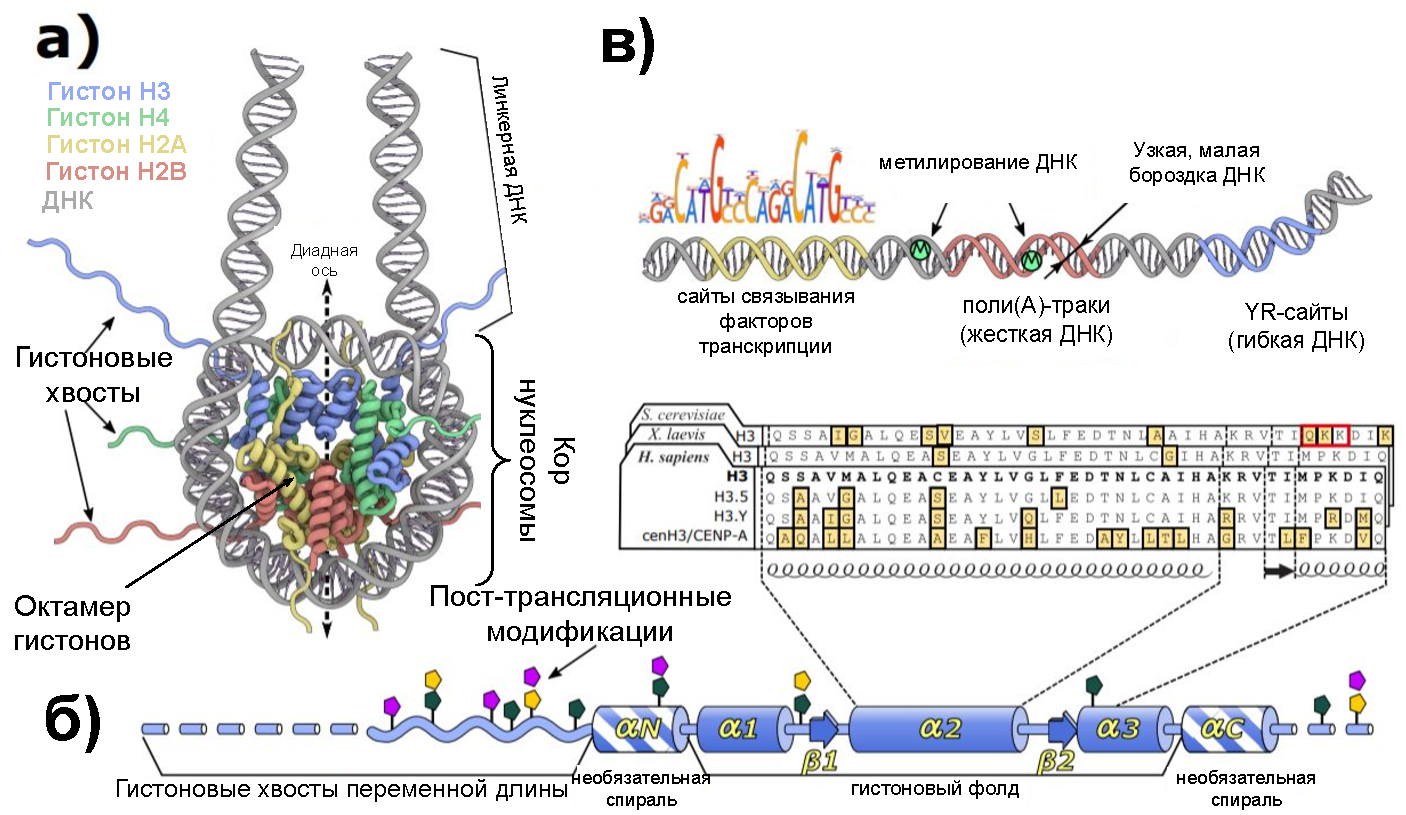
\includegraphics [width=\textwidth]{images/p2/cosb/part2_1_f1.pdf}
    \caption[Структура и вариабельность нуклеосомы]{(a) Структура нуклеосомы состоит из коровой частицы нуклеосомы (NCP), фланкированной линкерными сегментами ДНК. Коровая частица образована октамером гистонов, вокруг которого обернуты 145–147 пар оснований ДНК в виде левой суперспирали. Октамер состоит из двух пар гетеродимеров гистонов (H3-H4 и H2A-H2B) и обладает осью псевдосимметрии второго порядка (диадной осью), проходящей через центральную пару оснований нуклеосомной ДНК (диаду). Неструктурированные гистоновые хвосты отходят от глобулярной части белков. Малая бороздка ДНК обращена к октамеру гистонов в 14 специально предназначенных для этого сайтах связывания (в каждом сайте связывания боковая цепь остатка аргинина вставлена в малую бороздку). 
    (б) Схема типичной структуры гистонового белка: гистоновый фолд (спирали $\alpha$1, $\alpha$2 и $\alpha$3, листы $\beta$1 и $\beta$2) с необязательными спиралями $\alpha$N, $\alpha$C и гистоновыми хвостами переменной длины. Гистоновые ПТМ могут располагаться по всей длине белка и играть важную роль в функционировании хроматина, обеспечивая эпигенетическую разметку. Вариации гистонового сиквенса существуют как между организмами, так и внутри организма (гистоновые варианты).
    (в) ДНК - ключевой компонент нуклеосомы. Конкретные последовательности ДНК могут обеспечивать присутствие сайтов связывания факторов транскрипции в областях нуклеосомной ДНК, повышенную жесткость и/или изменения геометрии ДНК.}
    \label{fig:part2_1_f1}
\end{figure}



\subsection{Обзор динамических мод нуклеосом}

    Внимание на динамическую природу нуклеосом впервые было обращено в контексте отворачивания ДНК от октамера гистонов \cite{polach_mechanism_1995} (Рис. \ref{fig:part2_1_f2}a, в центре). Результаты экспериментов по ферментативному расщеплению ДНК \cite{polach_mechanism_1995}, измерению FRET \cite{li_nucleosomes_2004}, крио-ЭМ \cite{bilokapic_histone_2018} свидетельствуют о возможности откручивания ДНК (иногда называемом раскручиванием или дыханием ДНК). Данные процесс важен для доступа факторов транскрипции \cite{zaret_pioneer_2016,li_nucleosomes_2004} и РНК-полимераз \cite{bondarenko_nucleosomes_2006} к последовательности ДНК. Позднее выяснилось, что откручивание ДНК может происходить вместе с раскрытием димера H2A-H2B (состояние ``бабочка'') \cite{bohm_nucleosome_2011} или его полной диссоциацией (с образованием гексасомы), что часто происходит при транскрипции \cite{kireeva_nucleosome_2002}. Частично собранные нуклеосомы (также называемые субнуклеосомными структурами), такие как тетрасома или гемисома (полунуклеосома) также эффективно способствуют отворачиванию ДНК \cite{rychkov_partially_2017}. Недавно с использованием метода ChIP-exo было показано, что такие структуры широко распространены в динамическом хроматине в масштабе всего генома  \cite{rhee_subnucleosomal_2014}. В то время как тетрасомы могут возникнуть из-за потери двух димеров H2A-H2B нуклеосомой, динамические пути, ведущие к гемисомам, не совсем ясны. Новые экспериментальные данные подтверждают идею о том, что сборка нуклеосом \textit{in vivo} во время репликации ДНК происходит через депонирование тетрамеров H3-H4 (два димера H3-H4, взаимодействующие через четырехспиральную связку) с помощью фактора сборки хроматина 1 (CAF1) \cite{sauer_insights_2017,mattiroli_dna-mediated_2017}. После этого к ним присоединяются димеры H2A-H2B. Следовательно, маловероятно, что гемисомы образуются во время регулярной сборки нуклеосом. Расщепление нуклеосом на полунуклеосомы во время транскрипции - еще одна гипотеза (рассмотренная в \cite{zlatanova_nucleosome_2009}). Хотя есть некоторые споры, частным случаем статической структуры полунуклеосом могут быть центромерные нуклеосомы \textit{S. cerevisiae} \cite{henikoff_remarkable_2017}, которые также могут быть воссозданы \textit{in vitro} в особых условиях \cite{furuyama_reconstitution_2013}. В то время как нуклеосома в отсутствие внешнего сверхспирального стресса содержит ДНК в виде левосторонней суперспирали \cite{bancaud_structural_2006}, тетрасомы или гемисомы демонстрируют повышенную тенденцию к адаптации правостороннего состояния. Вероятно, так обстоит дело с центромерными нуклеосомами пекарских дрожжей [\textit{ibid.}] и тетрамерами гистонов архей \cite{marc_archaeal_2002}.



    В левой части рисунка \ref{fig:part2_1_f2} мы сгруппировали динамические режимы с меньшей величиной конформационных изменений (``компактная нуклеосома''), которые, тем не менее, функционально важны. Октамер гистона способен к ``расщеплению'' - изменению расстояния между двумя половинками нуклеосомы вдоль оси суперспирали ДНК. Экспериментально это наблюдалось на  нуклеосомах \cite{ngo_nucleosomes_2015,falk_cenp-c_2015} и может быть связано со скольжением витков ДНК относительно друг друга \cite{falk_cenp-c_2016}. Недавно наше понимание динамики октамера было дополнительно расширено за счет концепции пластичности октамеров на уровне отдельных димеров гистонов - точечные сшивки внутри димера H3-H4 ограничивает его деформируемость и ингибируют передвижение нуклеосом ремоделером SNF2h \cite{sinha_distortion_2017}. Наконец, ДНК в нуклеосоме - это компонент, который проявляет конформационную изменчивость. Октамер может скользить по ДНК, изменяя ротационное и трансляционное позиционирование ДНК \cite{shaytan_hydroxyl-radical_2017,shaytan_structural_2018}. Этот процесс сильно зависит от последовательности ДНК (обзор см. в \cite{eslami-mossallam_nucleosome_2016}) и включает локальные деформации ДНК, такие как дефекты скручивания \cite{edayathumangalam_nucleosomes_2005}. В линкерной области ДНК более гибкая, чем остальная часть ДНК \cite{gansen_structural_2009}. Благодаря такой высокой мобильности, комплексы нуклеосом с линкерным гистоном могут образовывать ансамбль различных конфигурации (см. обзор в \cite{ozturk_toward_2018}).


\begin{figure} [H]
    \centering
    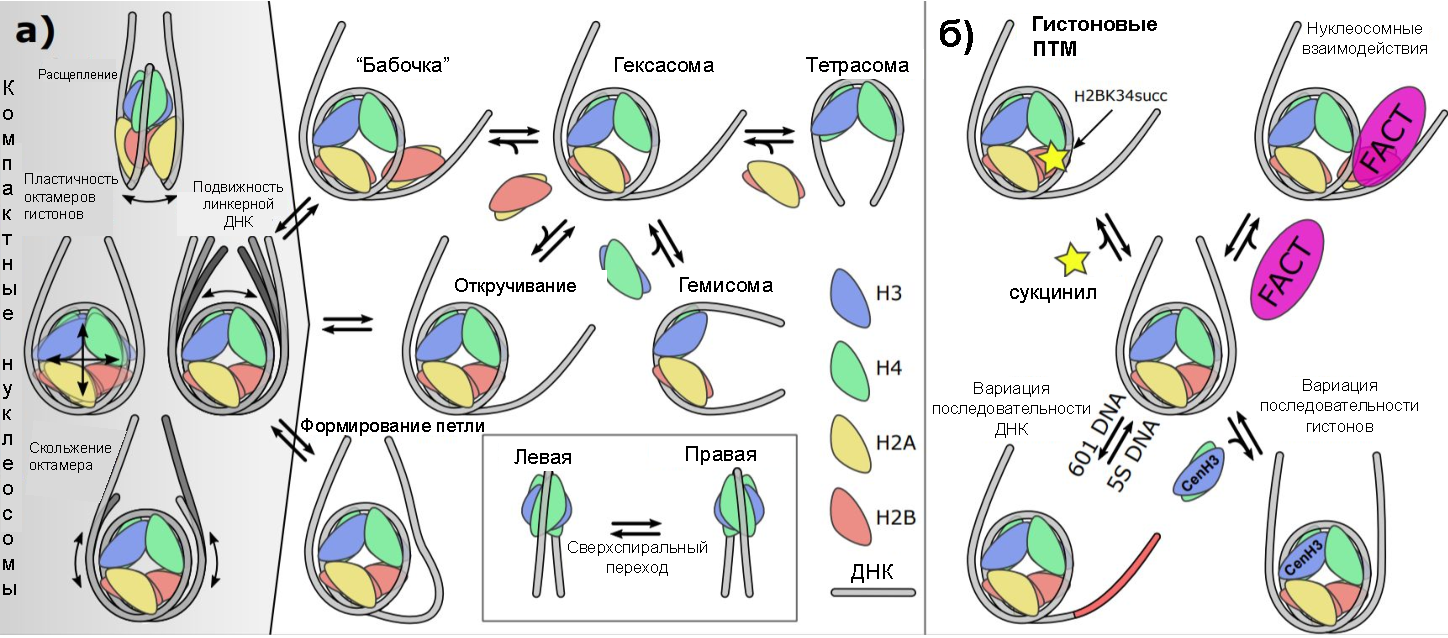
\includegraphics [width=\textwidth]{images/p2/cosb/part2_1_f2.pdf}
    \caption[Моды динамики нуклеосом]{(а) Обзор различных мод динамики нуклеосом. Слева (серая область) показаны режимы, сохраняющие компактность нуклеосомы. Справа показаны моды с большей амплитудой: нуклеосомная ДНК может спонтанно образовывать петли или отворачиваться от гистонов; большие состояния разворачивания ДНК способствуют образованию субнуклеосомных частиц: гексасом, тетрасом, гемисом.
    (б) Примеры факторов, влияющих на структурную динамику нуклеосом. Слева вверху: сукцинилирование H2B по лизину 34 способствует разворачиванию ДНК \cite{jing_site-specific_2018}. Справа вверху: ассоциация с фактором транскрипции FACT изменяет динамику развертывания нуклеосом \cite{valieva_large-scale_2016}. Слева внизу: разные последовательности ДНК имеют разную динамику разворачивания \cite{mauney_local_2018}. Справа внизу: вариант гистона H3 человека CENP-A изменяет подвижность линкерной ДНК \cite{roulland_flexible_2016}.}
    \label{fig:part2_1_f2}
\end{figure}


\subsection{Факторы, влияющие на динамику нуклеосом: недавние примеры}

    Факторы, влияющие на динамику нуклеосом можно разделить на четыре группы (Рис. \ref{fig:part2_1_f2}б): вариации последовательностей гистонов, вариации последовательности ДНК, ПТМ гистонов и различные белки, взаимодействующие с нуклеосомами.

     Белки, взаимодействующие с  нуклеосомами, включают в себя структурные белки хроматина (включая линкер гистона H1 \cite{lyubitelev_structure_2016}), шапероны гистонов, факторы транскрипции (включая пионерские факторы транскрипции \cite{zaret_pioneer_2016}), компоненты репликационного, транскрипционного и эпигенетического аппарата. Они могут влиять на любой из обсуждаемых режимов динамики нуклеосом. Например, гистоновый шаперон FACT обратимо разворачивает нуклеосомную ДНК с обоих концов \cite{valieva_large-scale_2016}, чтобы облегчить обмен димера гистона H2A-H2B \cite{wang_histone_2018}. Гистоновый шаперон Nap-1 является другим примером, он вытесняет димер H2A-H2B из нуклеосомы, и может действовать без необходимости изначального отворачивания ДНК \cite{lee_single-molecule_2017}. Показано, что на раскрытие центромерных нуклеосом влияет взаимодействие с белком CENP-C \cite{falk_cenp-c_2015}. Напротив, ПАРП-1 (многодоменный белок, который управляет обнаружением одно- и двухцепочечных разрывов во время репарации ДНК) значительно увеличивает расстояние между супервитками нуклеосомной ДНК в обратимой манере \cite{sultanov_unfolding_2017}. Линкерные участки ДНК могут притягиваться друг к другу гистоном H1, который снижает их гибкость \cite{bednar_structure_2017}.

    Неструктурированные гистоновые хвосты исторически были основными целями для исследования эффектов различных PTM гистонов на динамику нуклеосом \cite{bowman_post-translational_2015} (Рис. \ref{fig:part2_1_f1}б). По умолчанию считается, что модификации, изменяющие заряд (например, ацетилирование лизина, фосфорилирование серина или отщепление гистонового хвоста), вызывают дестабилизацию нуклеосом за счет снижения не-специфического электростатического притяжения между ДНК и гистонами \cite{fenley_modulation_2018}. Однако существуют свидетельства в пользу того, что более тонкие эффекты также могут иметь значение, такие как изменения вторичной структуры гистоновых хвостов (напр., для H4K16ac \cite{potoyan_regulation_2012}). ПТМ, расположенные на сайтах связывания гистонов с ДНК, могут оказывать более специфические эффекты, нарушая связывание с ДНК соответствующих местах. Например, недавно проанализированное сукцинилирование H2BK34, расположенного в сайте связывания ДНК гистонами на расстоянии $\sim$25 п.н. от точки входа/выхода в нуклеосоме, ингибирует сборку нуклеосом и способствует разворачиванию ДНК \cite{jing_site-specific_2018}. Важность ПТМ гистонов, локализованных в глобулярной части гистонов, и их функциональное значение в настоящее время также широко признаны. Например, H3K56ac облегчает разворачивание нуклеосом и играет важную роль в регуляции сборки нуклеосом \cite{zhang_multisite_2018}. Не изменяющие заряд ПТМ, такие как H3R42me2, также могут способствовать дестабилизации нуклеосом \cite{casadio_h3r42me2a_2013}; последний также использовался микобактериями для изменения эпигенетического ответа хозяина \cite{yaseen_mycobacteria_2015}. ПТМ на границах раздела гистон-гистон могут как нарушать образование октамера \cite{ye_histone_2005}, так и стабилизировать нуклеосомы (например, H4K77ac из-за устранения электростатического отталкивания внутри димера гистона \cite{fenley_modulation_2018}). Сходным образом, H1K85ac ведет к общей стабилизации хроматина и линкерной ДНК за счет увеличения связывания глобулярного домена H1 с коровыми гистонами \cite{li_histone_2018}.

    Нет сомнений в том, что вариация последовательности ДНК может оказывать значительное функциональное воздействие, изменяя вероятность разворачивания ДНК и стабильность нуклеосом. Например, сильно взаимодействующая последовательность ``601'', если ее поместить на нуклеосому, образует полярный барьер для транскрипции \cite{bondarenko_nucleosomes_2006}. Это соответствует известному асимметричному разворачиванию последовательности ``601'' под напряжением \cite{ngo_asymmetric_2015} и в состоянии покоя. Последнее было недавно подтверждено малоугловым рассеянием рентгеновских лучей по сравнению с симметричным разворачиванием, наблюдаемым для 5S рибосомной последовательности \cite{mauney_local_2018}. Динамические эффекты также играют роль во время связывания факторов транскрипции, как первоначально было предложено J. Widom и соавторами \cite{polach_mechanism_1995}. Например, недавняя крио-ЭМ структура нуклеосомы, включающая энхансерную последовательность ALB1 (ALB1 является сайтом связывания для пионерского фактора транскрипции FoxA), аналогична структуре 601-нуклеосомы, но ДНК в области связывания FoxA является более подвижной, способствующей связыванию FoxA \cite{takizawa_cryo-em_2018}. Несмотря на многочисленные усилия, точная взаимосвязь между последовательностью ДНК и ее влиянием на динамику нуклеосом все еще не ясна. По данным некоторых работ присутствие гибких пиримидин-пуриновых динуклеотидов (YR) в сайтах связывания ДНК является важным фактором для позиционирования ДНК и силы связывания (Рис. \ref{fig:part2_1_f1}в) \cite{cui_structure-based_2010,segal_dna_2009}. Однако развитию более общих теоретических моделей в настоящее время препятствует отсутствие достаточно подробных и воспроизводимых экспериментальных наборов данных о связи последовательности ДНК с ее стабильностью на нуклеосоме \cite{eslami-mossallam_nucleosome_2016}. Атомистическое и крупнозернистое компьютерное моделирование может восполнить этот пробел: как недавно показали несколько исследований с использованием моделирования, в зависимости от физических свойств последовательности ДНК, ее транслокация может предпочтительно происходить через винтовой механизм ``распространения дефектов кручения'' или механизм ``повторного захвата петли'' \cite{lequieu_silico_2017,niina_sequence-dependent_2017}.

    Варианты гистонов обеспечивают богатый репертуар вариаций канонической гистоновой последовательности, варьирующийся от всего лишь нескольких аминокислотных различий (например, H3 vs H3.5) до довольно существенных различий, которые могут изменять несколько динамических режимов одновременно (Рис. \ref{fig:part2_1_f1}б). Напр., CENP-A (вариант, критический для образования центромер во время митоза) имеет более короткую спираль $\alpha$N, чем канонический H3. Эта особенность делает линкерную ДНК в CENP-A нуклеосомах более гибкой и влияет на связывание ДНК с гистонами \cite{roulland_flexible_2016}. Кроме того, CENP-A влияет на разворачивание ДНК и способствует образованию петель \cite{stumme-diers_nanoscale_2018}. Известно также, что нуклеосомы CENP-A демонстрируют расщепление половинок нуклеосомы вдоль оси суперспирали \cite{falk_cenp-c_2015}. Варианты с небольшими изменениями канонической гистоновой последовательности также могут быть функционально очень важными: H3.3 важен для пластичности нейронов \cite{maze_critical_2015}, H3.5 для сперматогенеза \cite{urahama_histone_2016}, а H3.Y изменяет регуляцию клеточного цикла \cite{wiedemann_identification_2010}. В последние годы было показано, что эти небольшие вариации последовательности могут влиять на стабильность и динамику нуклеосом. Например, H3.5-специфический остаток лейцина 103 дестабилизирует нуклеосому, что важно для процесса транскрипции в тестикулярных клетках человека \cite{urahama_histone_2016}. Как показано в \cite{kujirai_identification_2017}, в H3.Y метионин 124 способствует стабильной ассоциации тетрамера H3.Y-H4 с ДНК. Другой H3.Y-специфический остаток -- лизин 42 -- играет роль в придании гибкости линкерной ДНК. 
    
    Более того, оказывается, что небольшие вариации между последовательностями канонических гистонов, кодируемых разными копиями генов канонических гистонов у человека, также могут функционально влиять на стабильность нуклеосом. Вариации M51L и K99R в гене гистона HIST1H2AH (изоформа H2A1H) приводят к стабилизации нуклеосом и изменяют пролиферацию клеток \cite{bhattacharya_histone_2017}. Точно так же теперь описаны эффекты небольших вариаций между каноническими последовательностями у разных видов. Специфичный для грибов гистоновый мотив H3 QKK (Рис. \ref{fig:part2_1_f1}в), расположенный на оси диады нуклеосомы, вносит вклад в плохую сборку октамеров в нуклеосомах дрожжей \cite{leung_unique_2016}.


\subsection{Тонкие детали динамики нуклеосом}

    Если распечатать димеры гистонов на 3D-принтере то из можно собрать в октамера подобно конструктору LEGO (см. 3D-печатные модели нуклеосом на \url{https://github.com/intbio/nuclLEGO}). Этот взгляд на нуклеосому как на жесткую модульную структуру теперь уступает место альтернативному взгляду на нуклеосому как на динамическую сущность, где даже небольшие конформационные вариации функционально важны. В поддержку последней точки зрения мы обсудим несколько недавних наблюдений, представленных на рисунке \ref{fig:part2_1_f3}. Во-первых, динамика ДНК внутри нуклеосомы выходит за рамки простого разворачивания и может демонстрировать различные искаженные конформации, включая дефекты кручение и выпячивание ДНК вблизи точки входа/выхода. Такого рода изменения недавно наблюдались как при атомистическом моделировании \cite{shaytan_coupling_2016} (Рис. \ref{fig:part2_1_f3} a), так и на крио-ЭМ картах \cite{bilokapic_histone_2018} (Рис.\ref{fig:part2_1_f3}в). Более того, изменения в конформации ДНК связаны с тонкими изменениями конформации гистоновых белков. Например, как показано в крио-ЭМ, разворачивание 15 пар оснований ДНК с одной стороны октамера гистонов приводит к изменениям конформации гистонов вблизи точек входа / выхода с обеих сторон, а также сопровождается общим небольшим расширением октамера перпендикулярно оси симметрии нуклеосомы \cite{bilokapic_histone_2018}. Более того, определенная связь между перестройками гистонового ядра и конформацией ДНК также наблюдалась для полностью завернутого состояния (Рис.\ref{fig:part2_1_f3}г), было показано, что нуклеосомы могут сокращаться на 8\% вдоль оси диады и расширяться на 5\% в перпендикулярном направлении \cite{bilokapic_structural_2018}.

  Пластичность индивидуальных димеров гистонов также функционально важна. В дополнение к недавно продемонстрированной важности пластичности H3-H4 для ремоделирования нуклеосом \cite{sinha_distortion_2017}, с помощью твердотельного ЯМР было показано, что внутренняя динамика во временных масштабах от наносекунд до миллисекунд присутствует для гистона H4 в нуклеосомах \cite{shi_structure_2018}. Недавнее исследование метил-TROSY ЯМР показало, что мутантные нуклеосомы могут проявлять значительно повышенную динамику внутри гистонов H3-H4 \cite{kitevski-leblanc_investigating_2018}. Помимо H3-H4, пластичность H2A-H2B, по-видимому, также имеет решающее значение для сборки и функционирования нуклеосом. В частности, сборка нуклеосом \textit{in vitro} со сшитыми димерами H2A-H2B происходит только до стадии гексасом \cite{bilokapic_histone_2018}, а это означает, что для сборки требуется определенная гибкость димера. Структура ЯМР  изолированного димера H2A-H2B в растворе, вероятно, отражает эти динамические режимы и демонстрирует повышенную гибкость и беспорядок, в частности, внутри дополнительных спиралей $\alpha$C и $\alpha$N по сравнению со структурой внутри нуклеосомы (Рис.\ref{fig:part2_1_f3}е) \cite{moriwaki_solution_2016}. Динамика H2A-H2B также, вероятно, используется ремоделером SWR1. Он распознает специфически канонические нуклеосомы, содержащие H2A, и заменяет H2A его вариантом H2A.Z. Способность ремоделера SWR1 распознавать и действовать на нуклеосомы H2A на не на H2A.Z недавно была связана с отличием нескольких аминокислот между H2A и H2A.Z. Причем ни одна из этих аминокислот не экспонируется на поверхности нуклеосом \cite{ranjan_h2a_2015}. Поскольку рентгеновские исследования показывают очень похожую структуру нуклеосом H2A и H2A.Z \cite{suto_crystal_2000}, эти открытия подразумевают, что присутствует некая динамическая сигнатура, которая используется для распознавания нуклеосом H2A.
    
    Наконец, тонкая динамика гибких гистоновых хвостов с их способностью взаимодействовать с ДНК и другими белками формирует еще один уровень динамической сложности. Гистоновые хвосты и другие белки хроматина несут положительно заряженные остатки (особенно аргинины \cite{west_electrostatic_2010,dragan_energetics_2003}), которые предпочитают взаимодействовать с малыми бороздками ДНК как участками отрицательного электростатического потенциала (Рис. \ref{fig:part2_1_f3} б). Эти взаимодействия могут, в свою очередь, модулироваться ПТМ гистонов или AT-богатыми последовательности ДНК (что способствует образованию узких малых бороздок \cite{freeman_dna_2014} и может распознаваться некоторыми белками в контексте нуклеосом \cite{xiao_molecular_2017}) (Рис. \ref{fig:part2_1_f1} в). 



\begin{figure} [H]
    \centering
    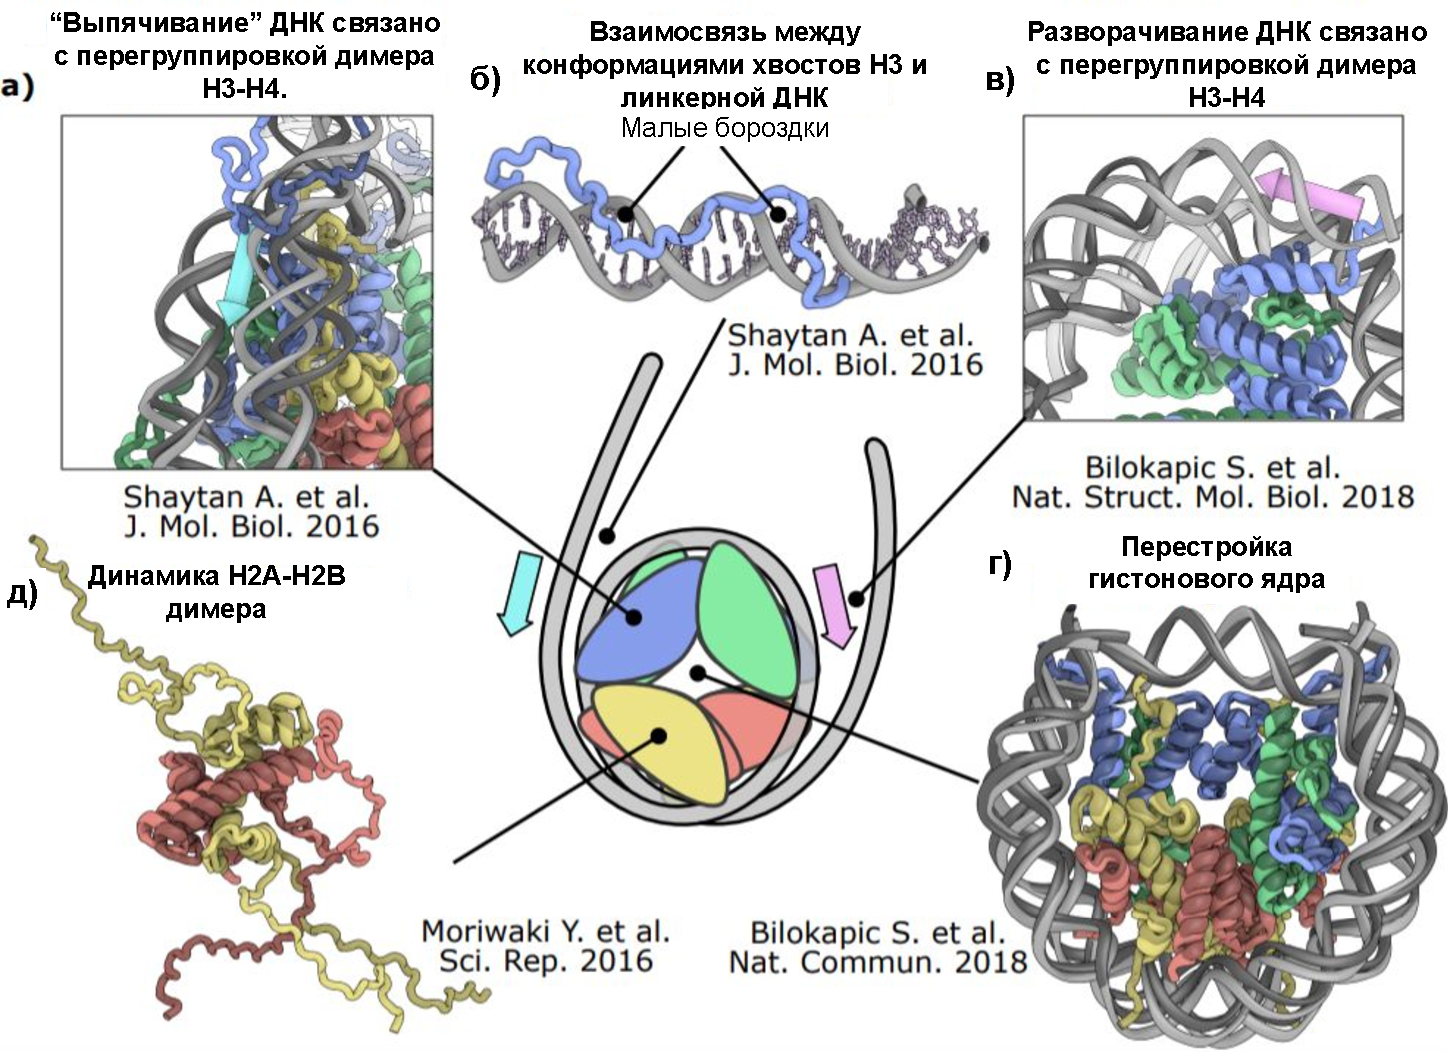
\includegraphics [width=\textwidth]{images/p2/cosb/part2_1_f3.pdf}
    \caption[Тонкие детали динамики нуклеосом]{Динамика ДНК в нуклеосомах тесно связана с динамикой гистонов (a, б, в, г). Цветовая схема соответствует рисунку \ref{fig:part2_1_f1}. Голубые и фиолетовые стрелки на центральной диаграмме и панелях (а) и (в) обозначают одни и те же области входа / выхода ДНК в нуклеосому. (а) Помимо простого разворачивания ДНК, ДНК может проявлять выпуклости возле точек входа / выхода, как это наблюдается в моделировании МД и крио-ЭМ \cite{bilokapic_histone_2018,shaytan_coupling_2016}.  (б) Гистоновый хвост H3 взаимодействует с линкерным сегментом ДНК. Наблюдаются преимущественные взаимодействия с малыми бороздками ДНК \cite{shaytan_coupling_2016}.
    (в) Раскручивание ДНК  сопровождается перестройками в димере гистона H3-H4 \cite{bilokapic_histone_2018}. Кристаллическая структура нуклеосомы показана светлыми цветами. 
    (г) Гистоновый октамер с полностью обернутой ДНК может принимать сжатую конформацию вдоль оси диады (темные цвета) по сравнению с кристаллической структурой по умолчанию (светлые цвета) \cite{bilokapic_structural_2018}. 
    (д) Гибкость димера гистона H2A-H2B, наблюдаемая с помощью ЯМР-исследований в растворе \cite{moriwaki_solution_2016}. Две конформации показаны темным и светлым цветами.}
    \label{fig:part2_1_f3}
\end{figure}
















% COSB - последний

\section{Моделирование нуклеосом с линкерными участками ДНК}
\textit{Данный раздел написан по материалам статей \cite{shaytan_coupling_2016,shaytan_trajectories_2016}, результаты которых основаны в том числе на предыдущих работах \cite{armeev_conformational_2015,armeev_molecular_2015,gribkova_investigation_2017,armeev_nucleosome_2016}.}

%\todo{2S - сюда нужно вставить переведенные текст с картинками materials\/jmb\_2016\/paper.docx, картинки нужно засунуть в гугл Draw (папка p2) - там перевести наложив поверх английского текста русский. Ссылки на литературу уже загружены в зотеро (если вдруг чего-то нет, нужно написать мне). Все заголовки начинать с уровне subsection и далее}

    При формировании нуклеосом октамер гистоновых белков организует около 200 пар оснований ДНК в два суперспиральных витка. Хотя статическая структура коровой частицы нуклеосомы была разрешена, детали динамических взаимодействий между гистонами и ДНК остаются не совсем понятными. Для изучения данного вопроса мы провели длительное равновесное моделирование молекулярной динамики нуклеосом, включая линкерные сегменты ДНК и полноразмерные гистоны, в явном растворителе в атомистическом приближении. Впервые мы смогли идентифицировать и охарактеризовать перестройки в нуклеосомах на микросекундном масштабе времени, изучить связь между конформацией гистоновых хвостов и геометрией ДНК. Мы обнаружили, что определенные конформации гистонового хвоста способствовали выпячиванию ДНК вблизи участков ее входа/выхода в/из нуклеосомы, что приводило к образованию дефектов кручения внутри ДНК. Мы охарактеризовали динамику гистоновых хвостов при их конденсации на нуклеосомальной и линкерной ДНК и показали, что хвосты могут принимать конформационно ограниченные позиции из-за вставки  лизинов и аргининов в малые бороздки ДНК. Потенциально, эти явления влияют на доступность посттрансляционно модифицированных остатков гистонов, которые служат важными сайтами для эпигенетических меток (например, в H3K9, H3K27, H4K16). Предполагается, что взаимодействия гистоновых хвостов с коровой и линкерной ДНК модулируют процессы взаимодействия белков хроматина с гистонами, модификации хвостов и связывания эффекторных белков. В данном разделе мы обсуждаем влияние наблюдаемых явлений на функцию нуклеосом и сравниваем наши результаты с различными экспериментальными исследованиями.

\subsection{Введение}
    Нуклеосомы - это элементарные единицы компактизации хроматина в геномах эукариот, расположенные через каждые 200 $\pm$ 40 п.н. вдоль ДНК \cite{mcghee_nucleosome_1980}. Основным источником информации об атомистической структуре нуклеосомы являются рентгеновские исследования коровых частиц нуклеосом (NCP) (см. обзор \cite{dechassa_nucleosomes_2011}), которые неизменно разрешают очень похожие структуры гистонов и ДНК независимо от вариантов последовательности гистонов, мутаций, посттрансляционные модификации, последовательности ДНК или присутствия белков, связывающих нуклеосомы, пептидов или химических агентов. Например, суперпозиция различных структур нуклеосом с использованием алгоритма VAST+ \cite{madej_mmdb_2014} показала очень небольшие вариации в среднеквадратичном отклонении (RMSD) около 1 \AA для выровненных глобулярных частей гистоновых областей. Консенсусная структура NCP формируется путем наматывания $\sim$ 145-147 п.н. коровой ДНК в $\sim$ 1,7 левых сверхспиральных витка вокруг октамера, состоящего из четырех типов коровых гистонов (H3, H4, H2A, H2B) \cite{marino-ramirez_histone_2011}. Структура NCP характеризуется наличием диадной оси - оси псведосимметрии второго порядка, сильно изогнутой структурой ДНК \cite{tolstorukov_novel_2007} и высоким положительным зарядом октамера гистонов \cite{fenley_charge_2010}. Кроме того, он включает большое количество молекул воды, проникающих в структуру нуклеосомы \cite{davey_solvent_2002}, а также длинные гистоновые хвосты, выступающие из ядра нуклеосомы и обеспечивающие множество сайтов для посттрансляционных модификаций (ПТМ).

    С другой стороны, решающая роль нуклеосом в функционировании хроматина (включая тонкую регуляцию экспрессии генов, репликацию ДНК, репарацию и наследование, опосредованные эпигенетическими механизмами \cite{henikoff_nucleosome_2008,petty_balancing_2013}) зависит от их динамической природы и конформационных переходов. Действительно, многие биофизические (FRET, эксперименты с одномолекулярными пинцетами и другие, рассмотренные в \cite{choy_structural_2012}) и биохимические эксперименты (анализ связывания факторов транскрипции \cite{li_rapid_2005}, химическая сшивка \cite{lee_n-terminal_1997}, анализ методом ChIP-exo  \cite{rhee_subnucleosomal_2014}) предполагают, что нуклеосомы демонстрируют существенный конформационный полиморфизм как на локальном (конформация ДНК и гистоновых хвостов внутри нуклеосомы), так и на глобальном (потеря гистонов, субнуклеосомные частицы и т. д.) масштабах, которые, в свою очередь, могут быть результатом равновесных тепловых флуктуаций или могут быть активно индуцированы внешними силами внутри клетки.
    
    Были предложены различные функционально значимые моды динамики нуклеосом, которые включают дыхание/разворачивание/раскрытие ДНК, расщепление нуклеосом \cite{zlatanova_nucleosome_2009}, а также скольжение нуклеосом \cite{mueller-planitz_nucleosome_2013}, раскрытие или потерю димера H2A-H2B \cite{shaytan_nucleosome_2015}. В то же время, различные конформационные перестройки гистоновых хвостов необходимы для внутри- и межнуклеосомных взаимодействий \cite{pepenella_intra-_2014}, для множественных взаимодействий с ремоделерами хроматина \cite{hwang_histone_2014,racki_histone_2014}, гетерохроматиновыми белками \cite{wang_heterochromatin_2013} и со многими эффекторными белками, которые содержат домены, связывающие модификации гистонов \cite{rando_combinatorial_2012}. Тем не менее, взгляду на нуклеосомы как на динамические объекты \cite{zlatanova_nucleosome_2009} все еще не хватает понимания деталей на атомистическом уровне.

    Чтобы попытаться сгладить этот очевидный пробел в нашем понимании динамики и функций нуклеосом, уже были предприняты значительные усилия в области моделирования, включая моделирование молекулярной динамики (МД) на атомистическом уровне \cite{biswas_atomistic_2013} и моделирование в крупнозернистом приближении \cite{arya_role_2006,collepardo-guevara_chromatin_2014}. Однако из-за значительного размера нуклеосомы по стандартам атомистического моделирования и чрезвычайно долгих временных масштабов ее функциональной динамики в предыдущих исследованиях приходилось прибегать либо к крупнозернистому моделированию без атомистических деталей, либо к полностью атомному моделированию без явных молекул растворителя \cite{erler_role_2014}. Полноатомное моделирование проводилось на временах не превышающих нескольких сотен наносекунд \cite{materese_counterion_2009,ruscio_computational_2006}. Однако мы знаем, что изменения в атомных взаимодействиях могут иметь глубокие функциональные последствия для нуклеосом. Например, посттрансляционные модификации могут изменять внутри- и межнуклеосомные взаимодействия или обеспечивать множественные сайты связывания для так называемых эффекторных белков \cite{ruthenburg_multivalent_2007}, даже однократное ацетилирование H4K16 может запускать разворачивание хроматиновых волокон \cite{dorigo_chromatin_2003,norouzi_topological_2015-1}.

    В работе, изложенной в данном разделе, концептуальный прогресс состоит в том, чтобы использовать наиболее надежный подход моделирования методом МД с явным  растворителем для всех атомов  и расширить этот подход на значительно более длительную микросекундную шкалу времени. Микросекундное моделирование, а также модели нуклеосом с реалистичными сегментами ДНК-линкера и многочисленные сравнительные модели позволили нам получить представление о функционально значимых перестройках в нуклеосомах, включая связь между конформациями гистоновых хвостов и геометрией ДНК. Хотя многие функционально релевантные движения могут происходить в гораздо более длительных временных масштабах \cite{choy_structural_2012}, несколько недавних исследований ЯМР показали, что гистоновые хвосты демонстрируют субмикросекундную динамику, что дает возможность сравнить наши расчетные результаты с экспериментальными данными \cite{kato_characterization_2009,zhou_histone_2012,gao_histone_2013}.

    В этом исследовании мы обнаружили, что определенные конформации гистонового хвоста способствуют выпячиванию ДНК возле мест входа/выхода ДНК в нуклеосоме, образованию дефектов кручения внутри ДНК и перестройке взаимодействий гистонов с ДНК в нуклеосомном коре. Мы охарактеризовали динамику гистоновых хвостов при их конденсации на коровой и линкерной ДНК на атомистическом уровне и показали, что они могут принимать конформационно ограниченные положения, сопровождаемые вставкой определенных ``закрепляющих'' лизинов и аргининов в малые бороздки ДНК. Мы предполагаем, что эти процессы влияют на доступность посттрансляционно модифицированных остатков гистонов, которые служат важными эпигенетическими метками (например, H3K9, H3K27, H4K16), а взаимодействия с коровой и особенно линкерной ДНК (для хвоста H3) могут модулировать доступность различных сайтов на гистоновых хвостах для связывания эффекторными белками.

\subsection{Результаты}

\subsubsection{Обзор исследованных моделей}
В нашем исследовании мы использовали несколько систем для моделирования, в том числе специально сконструированную полную нуклеосомную систему с линкерными сегментами ДНК по 20 п.н., фланкирующих коровую частицу с каждой стороны (модель FN) (Рис. \ref{fig:p2_2_f1}а), минималистичную модель коровой частицы с усеченными гистоновыми хвостами (NCPm модель) и набор вспомогательных систем с различными условиями моделирования (подробности см. в таблице \ref{tbl:p2:jmb_t1}). Ниже мы в основном сосредотачиваемся на результатах, полученных для полной нуклеосомной системы, для которой были выполнены обширные микросекундные расчеты. Мы допускаем, что динамика нуклеосом происходит в нескольких временных масштабах, а функционально значимые конформационные переходы часто превышают масштаб времени в одну микросекунду. Наше моделирование ограничивалось исследованием конформационных ансамблей вокруг определенных локальных квазиравновесных состояний в микросекундной шкале времени. Поэтому, интерпретируя результаты нашего моделирования, проверяли наши выводы, выполняя несколько вспомогательных расчетов. При обсуждении результатов ниже мы ссылаемся на ключевые структурные элементы гистоновых последовательностей и нуклеосом, как показано на рисунке \ref{fig:p2_2_f2} (см. Также раздел ``Название элементов структуры нуклеосом'' ниже).


\begin{table}[p]
\caption{Исследованные в моделировании системы и их параметры}
	\label{tbl:p2:jmb_t1}	
	\begin{tabularx}{\textwidth} { 
  | >{\raggedright\arraybackslash}X 
  | >{\centering\arraybackslash}X 
  | >{\raggedleft\arraybackslash}X 
  | >{\raggedleft\arraybackslash}X 
  | >{\raggedleft\arraybackslash}X 
  | >{\raggedleft\arraybackslash}X |}
  \hline
Название & Описание & Количество атомов, тыс. & Эффект. концентрация соли, мМ & Размер ячейки, \AA & Время моделирования, нс\\
	\hline

FN & Система с линкерной ДНК и гистоновыми хвостами & 366,8 & $\sim$185 & 162х197х113 & 1000 \\
\hline
FN1M & То же, что и не FN, но в высокой концентрации соли & 366,8 & $\sim$1100 & 161х196х112 & 1000 \\
\hline
FNbb & То же, что и не FN, но в большей ячейке & 3200 & $\sim$160 & 322х358х274 & 1000 \\
\hline
FNnt & То же, что и не FN, но с ацетильными и N-метил группами на концах гистонов& 366,8 & $\sim$185 & 162х197х113 & 1000 \\
\hline
NCPm & Cистема, без линкерной ДНК и хвостов гистонов & 310,3 & $\sim$200 & 145х141х101 & 1000 \\
\hline

\end{tabularx}
	 
\end{table}

\begin{figure} [H]
    \centering
    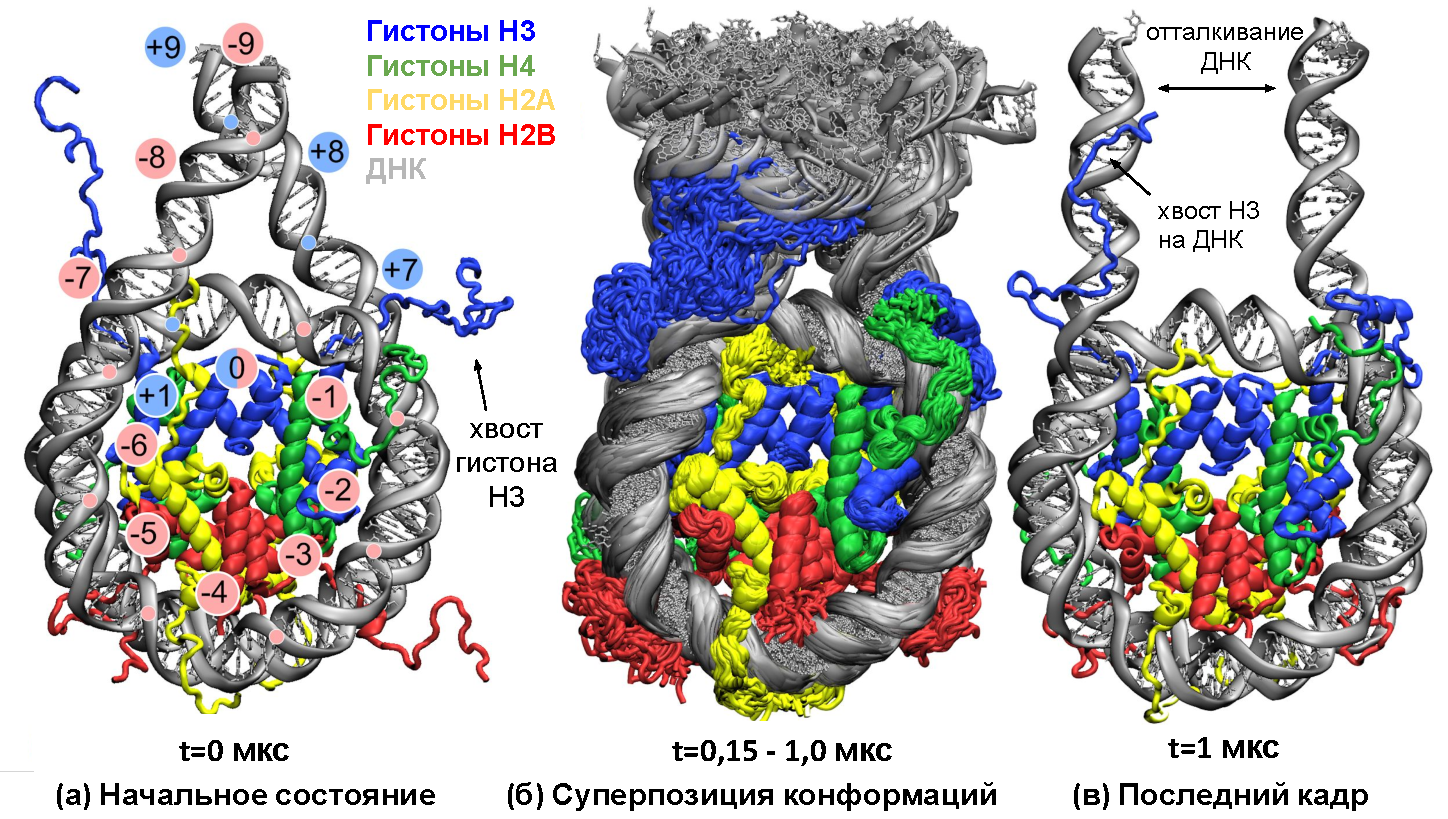
\includegraphics[width=\textwidth]{images/p2/jmb/part2_2_f1.pdf}
    \caption[Обзор структуры и динамики модели полной нуклеосомы (FN)]{Обзор структуры и динамики модели полной нуклеосомы (FN): (a) Исходная структура модели FN, (б) наложенные конформации из последних 75 \% кадров расчетной траектории, (в) последний кадр после 1 мкс, обратите внимание на различные формы N-концевых хвостов H3 с обеих сторон.}
    \label{fig:p2_2_f1}
\end{figure}

\begin{figure} [H]
    \centering
    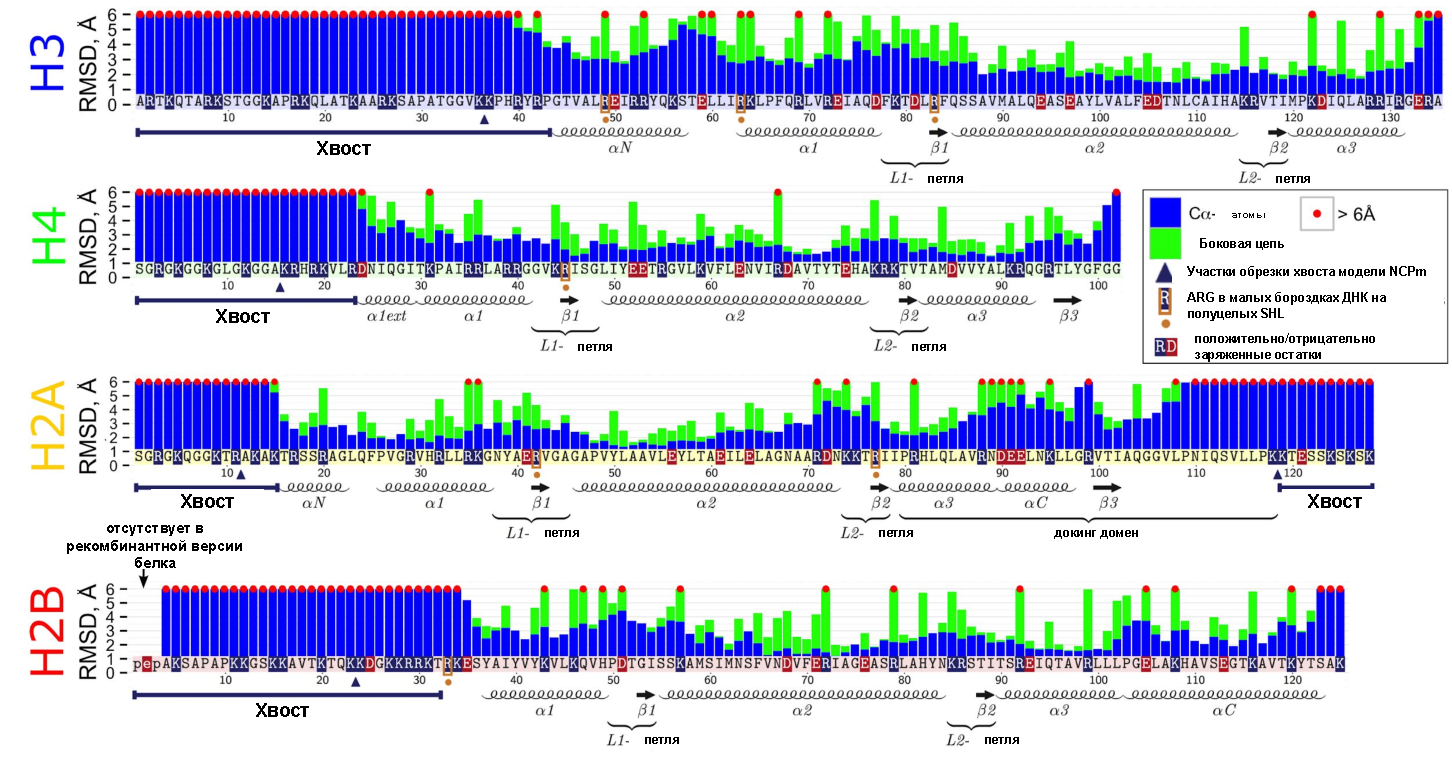
\includegraphics[width=\textwidth]{images/p2/jmb/part2_2_f2.pdf}
    \caption[Максимальные наблюдаемые среднеквадратичные отклонения отдельных аминокислот гистонов 
    в МД моделировании]{Максимальные наблюдаемые среднеквадратичные отклонения отдельных 
    аминокислот (C$\alpha$-атомы - синие столбцы, атомы боковой цепи - зеленые столбцы) во время
     моделирования относительно их положения в исходной рентгеновской структуре. 
     Значения, превышающие 6\AA, усекаются при этом значении и отмечаются красной точкой над столбцом.
      Аннотации структурных элементов гистонов приведены под столбиками.}
    \label{fig:p2_2_f2}
\end{figure}



\subsubsection{Конформационная стабильность и пластичность гистонов и ДНК}

    В соответствии с предыдущими экспериментальными исследованиями, наше моделирование подтвердило общую стабильность ядра нуклеосомы в отношении диссоциации компонентов нуклеосомы или крупномасштабного развертывания ДНК (см. Обзор динамики на рисунке \ref{fig:p2_2_f1}). В целом, RMSD центральной области гистонов оставалось в среднем в пределах 1,5\AA от кристаллографических положений для всех изученных моделей. Это было верно даже для минималистичной системы NCPm с усеченными гистоновыми хвостами. Таким образом, предполагается, что нуклеосомы имеют достаточный запас стабильности в отношении усечения гистоновых хвостов на микросекундных временах. Однако подробный анализ конформационной динамики, представленный ниже, предоставил новое понимание конформационной гибкости нуклеосом и выявил конформационные перестройки внутри гистонового ядра, гистоновых хвостов, ядра ДНК и линкерных областей, которые происходят в микросекундной шкале времени.

    Чтобы предоставить подробную картину динамики гистонов, мы изобразили максимальные отклонения позиций атомов, наблюдаемые в ходе динамики, от положений в кристаллической структуре (Рис. \ref{fig:p2_2_f2}). Как можно видеть на рисунке \ref{fig:p2_2_f2}, относительно большие конформационные изменения более чем на 6\AA наблюдались для атомов остова всех хвостов гистонов, даже некоторые части гистоновых фолдов демонстрируют высокое RMSD. Хотя, как показывает анализ кристаллических структур, докинг домен H2A (docking domain) образует тесные контакты с тетрамером $(H3-H4)_2$ \cite{suto_crystal_2000}, мы продемонстрировали существенные конформационные изменения для С-концевой части этого домена относительно исходной кристаллической структуры. Конформационные флуктуации остова белковой цепи часто сопровождались переориентацией боковых цепей аминокислотных остатков. Например, изменения в $\alpha$C-спирали докинг-домена сопровождались временным образованием новых солевых мостиков между H2A R88 и R99, фланкирующими эту спираль, и H3 E105, D106. Наблюдаемая пластичность докинг-домена будет влиять на его функции в качестве партнера по связыванию белков хроматина. В частности, недавно было показано, что шаперон ANP32E может быть ответственным за встраивание гистона H2A.Z в нуклеосому. ANP32E может связываться с $\alpha$C-спиральной областью докинг-домена H2A.Z \cite{obri_anp32e_2014}, которая в нуклеосоме структурно очень похожа на каноническую $\alpha$C-спираль H2A. Связывание гистона с ANP32E стерически несовместимо с полной структурой нуклеосомы и может запускать разборку и вытеснение нуклеосом, когда гибкая область ANP32E вставляется в кор нуклеосомы. Последний процесс не очень хорошо изучен, однако повышенная конформационная гибкость в этой области, наблюдаемая в нашем исследовании, указывает на возможные механизмы этого процесса. Интересно, что Biswas et al. в более ранних работах по МД моделированию нуклеосом показали потенциальную связь между усечением гистоновых хвостов H3 и конформациями боковых цепей H2A R81 и R88 \cite{biswas_role_2011}. Визуальное исследование траекторий динамики наших систем показывает, что, хотя боковая цепь H2A R88 очень гибкая в микросекундном масштабе времени, боковая цепь H2A R81 в основном заблокирована в своей кристаллографической ориентации и иногда перескакивает в положение, направленное в сторону от октамера гистонов. В последнем положении боковая цепь может находиться сотни наносекунд.

    Кроме того, значительные смещения остова полипептидной цепи (более 3\AA) и боковых цепей (более 6\AA) наблюдались в центральных областях других гистонов, включая H3 $\alpha$N-спираль, H3 $\alpha$1-спираль, сайт связывания L1-L2 димера H2A-H2B и H2B $\alpha$C-спираль) (Рис. \ref{fig:p2_2_f2}). Как уже упоминалось, даже если остов белка не демонстрирует больших отклонений от кристаллографических положений, все же могут происходить значительные изменения конформеров боковых цепей. Фактически, все аминокислоты, кроме одной, с наблюдаемой переориентацией боковой цепи более 6\AA, принадлежали заряженным остаткам. Эти переориентации часто включают разрушение и образование новых солевых мостиков внутри гистонового ядра. Изменения в модели NCPm показали аналогичные закономерности.


    Анализ конформационной динамики коровой и линкерной ДНК показал, что ДНК оставалась в среднем в пределах 4\AA (5 \AA для модели NCPm) от своих кристаллографических положений, измеренных с помощью RMSD атомов N1 и N9 азотистых оснований. Кроме того, фосфатный остов ДНК характеризуется периодическим профилем средних флуктуации (RMSF): участки остова ДНК, контактирующие с гистонами, проявляли значительно меньшие колебания по сравнению с теми, которые были обращены в раствор. С другой стороны, линкерные сегменты ДНК в нашем моделировании явно демонстрировали гораздо более сильные колебания, чем коровые участки ДНК (Рис. \ref{fig:p2_2_f1}б,в), что согласуется с известными данными \cite{pachov_structure_2011}. Глобальная конформация ДНК была дополнительно изучена с помощью 2D-проекций многоугольников, соединяющих центры пар оснований ДНК в нуклеосомной суперспиральной системе отсчета (см. Рис. \ref{fig:p2_2_f3}). Позиционные колебания линкерных сегментов ДНК охватывают частично перекрывающиеся конусообразные области в пространстве с угловым размахом около $\pm$45 градусов в обеих проекциях. Никаких существенных корреляций в позиционных колебаниях линкеров ДНК обнаружено не было. Средние положения, принятые для линкерных цепей ДНК в MD, были дальше друг от друга по сравнению с их исходными положениями, которые соответствовали прямому продолжению концов коровой ДНК (Рис. \ref{fig:p2_2_f3}а). Моделирование той же системы, но в солевом растворе с высоким содержанием 1 М (система FN1M) ясно показало, что два линкера ДНК приближаются друг к другу и даже большую часть времени взаимодействуют своими концами. Предполагаем, что скрининг электростатических взаимодействий значительно повлиял на угол входа/выхода ДНК. Интересно, что более ранние экспериментальные измерения расстояний между линкерами с помощью FRET показали, что расстояние монотонно уменьшается с увеличением концентрации соли \cite{toth_chromatin_2006}.

    Первостепенным вопросом динамики нуклеосом является амплитуда, временная шкала и механизмы отворачивания/дыхания ДНК, разворачивания или открытия поверхности октамера гистонов, что, как полагают, имеет решающее значение для доступности ДНК и связывания факторов транскрипции \cite{li_rapid_2005,mirny_nucleosome-mediated_2010}. К сожалению, на сегодняшний день нет полной картины, поскольку разные экспериментальные установки, интерпретация и терминология часто поддерживают разные взгляды на эту проблему \cite{choy_structural_2012,zlatanova_nucleosome_2009}. В этом исследовании мы не наблюдали крупномасштабного разворачивания или раскрытия коровой ДНК ни в системах FN, ни в системах NCPm. Такое разворачивание, если оно произойдет, обнажит достаточно частей ДНК для распознавания факторами транскрипции. Наши результаты согласуются с экспериментальными оценками временных масштабов событий разворачивания, которые лежат в субсекундном диапазоне \cite{li_rapid_2005,tomschik_nucleosome_2009}. Однако, если мы рассмотрим более умеренные колебания концов коровой ДНК вместе с линкерной ДНК (часто называемые ``дыханием ДНК''), такие процессы могут происходить в более коротких временных масштабах \cite{gansen_nucleosome_2009}. Например, недавние измерения FRET расстояний между двумя красителями, расположенными симметрично на обоих сегментах линкерной ДНК на расстоянии 5 п.н. от сайтов входа / выхода ДНК, показали две разные конформации с характерными расстояниями между двумя красителями $\sim$4,5 нм и $\sim$6,5 нм (амплитуда около 2 нм), в предположении  модели с двумя состояниями \cite{nurse_clipping_2013}. В нашем моделировании расстояние между центрами пар оснований соответствующих позиций линкеров ДНК варьировалось от 4,5 нм до 6,8 нм (см. Рис. \ref{fig:p2_2_f3}) (со средним значением 5,6 нм и RMSF 0,4 нм), показывая, что эти диапазоны расстояний находятся в пределах досягаемости быстрых субмикросекундных колебаний. Кроме того, мы наблюдали асимметрию в средних конформациях ДНК двух линкеров, а также в их отклонениях от исходной кристаллической структуры (обозначенной стрелками на рисунке \ref{fig:p2_2_f3}). Интересно, что если мы предположим, что наблюдаемые асимметрии соответствуют двум различным стабильным конформационным состояниям ДНК в нуклеосоме, переход между этими состояниями может уже объяснить изменение положения ДНК в  0,5 нм на расстоянии 5 п.н. от входа/выхода. Однако мы признаем, что методология для точного сравнения различных конформационных переходов, наблюдаемых при моделировании, и результатов измерений FRET все еще требует разработки и проверки: как недавно было отмечено Ленцем и др., флуктуация формы ДНК в нуклеосоме может размывать сигналы FRET от промежуточных конформационных состояний ДНК в нуклеосоме \cite{lenz_influence_2015}.

    В следующих разделах мы продемонстрируем, что эти конформационные асимметрии ДНК следствие асимметричной конденсацией гистоновых хвостов. Хотя мы находим, что время, необходимое для переключения между различными конформациями гистоновых хвостов, явно превышает микросекундную шкалу времени, мы предполагаем, что динамика ДНК в микросекундной шкале времени определяется взаимодействиями между гистоновыми хвостами и ДНК, которые, в свою очередь, могут влиять на конформацию ДНК на гораздо более длительных временах.
    %корявый перевод получился последнего абзаца, не понимаю как на русском правильно написать

\begin{figure} [H]
    \centering
    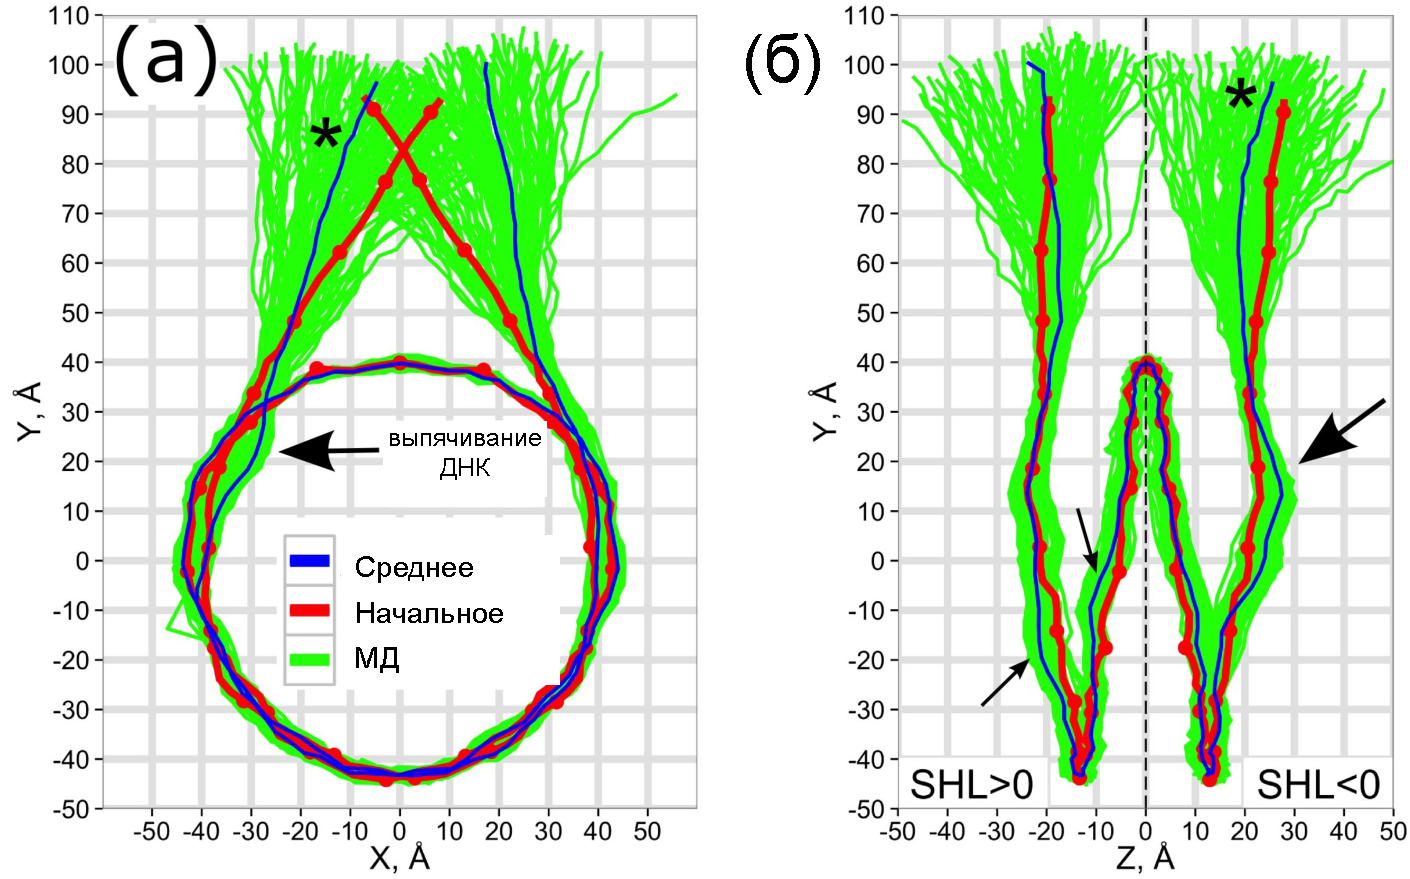
\includegraphics[width=\textwidth]{images/p2/jmb/part2_2_f3.pdf}
    \caption[Конформационный ансамбль ДНК в нуклеосоме]{Конформационный ансамбль ДНК в нуклеосоме, (а) - передняя и (б) - боковые проекции. Красными точками отмечены целые и полуцелые значения суперспирального положения (SHL) вдоль исходной конформации, звездочкой отмечен один линкерный сегмент ДНК на обоих рисунках. Стрелки указывают максимальные отклонения между исходной и средней конформациями в МД.}
    \label{fig:p2_2_f3}
\end{figure}

\subsubsection{Быстрая конденсация гистоновых хвостов на коровой и линкерной ДНК}
    Положительно заряженные гистоновые хвосты были тщательно изучены как экспериментально, так и с помощью методов моделирования. Известно, что межнуклеосомные взаимодействия опосредуются хвостами и играют важную роль в уплотнении хроматина. В этой работе мы охарактеризовали динамику взаимодействий между гистонами и ДНК на атомном уровне и обнаружили, что в среднем 60\% всех контактов были обеспечены взаимодействиями ДНК с участками гистонового хвоста. Хвосты гистонов, которые в исходной модели выступали в объем растворителя (в основном хвосты H3, Рис. \ref{fig:p2_2_f1}а), быстро адсорбировались на ДНК в течение первых 20 нс моделирования. От 50 до 90\% всех аминокислот в этих хвостовых областях имели прямые или опосредованные водой взаимодействия с коровой или линкерной ДНК в течение 1 мкс моделирования (Рис. \ref{fig:p2_2_f4}). Какого-либо существенного скопления контактов к началу или концу хвостов мы не наблюдали. Предыдущие полноатомные МД расчеты нуклеосомных частиц также указали на значительную ассоциацию гистоновых хвостов с коровой ДНК на временном масштабе 100 нс \cite{erler_role_2014,biswas_role_2011,roccatano_structural_2007}. Однако были высказаны определенные опасения по поводу коротких временных масштабов моделирования, а также артефактов, возникающих из-за периодических граничных условий и решеточных методов суммирования электростатических взаимодействий. Чтобы решить последнюю проблему, мы выполнили моделирование на протяжении 80 нс в большой ячейке (система FNbb), размер которой должен минимизировать потенциальные неблагоприятные эффекты периодических граничных условий. Моделирование FNbb подтвердило предпочтительную ассоциацию гистоновых хвостов с ДНК и быструю конденсацию длинных N-концевых хвостов H3. Таким образом, мы снимаем ранее высказанные опасения и показываем, что конденсация гистонового хвоста не является артефактом конкретных методов, используемых в МД-моделировании.

    Несколько исследований малоуглового рассеяния рентгеновских лучей (SAXS) касались вопроса о том, выступают ли гистоновые хвосты из ядра нуклеосомы в раствор или связаны с ДНК с физиологической ионной силой. Сообщалось о значительном увеличении максимального диаметра нуклеосом при повышении концентрации одновалентной соли с 10 мМ до физиологических концентраций и выше \cite{mangenot_salt-induced_2002}. Этот результат был приписан процессу диссоциации гистоновых хвостов от кора нуклеосомы. Однако Ян и др. \cite{yang_biophysical_2011} указали, что сопоставимое увеличение диаметра можно объяснить конформационными изменениями нуклеосом, включая разворачивание ДНК. Наши результаты подтверждают модель, в которой гистоновые хвосты прикреплены к коровой или линкерной ДНК большую часть времени в этой временной шкале. Если по какой-то причине хвосты оторвались, характерное время их присоединения должно составить около нескольких десятков наносекунд, о чем свидетельствует их быстрая конденсация (Рис. \ref{fig:p2_2_f4}). Наши теоретические оценки радиусов гирации предполагают, что и гистоновые хвосты, и линкерная ДНК вносят вклад в увеличение радиусов гирации.

    Чтобы дополнительно выяснить влияние концентрации соли на поведение хвоста, мы выполнили моделирование при чрезвычайно высокой концентрации соли 1M (модель FN1M). Хотя известно, что октамерная форма нуклеосом нестабильна при такой концентрации соли \cite{wilhelm_reconstitution_1978}, мы не наблюдали никакой разборки нуклеосом, что позволяет предположить, что это происходит во временном масштабе, намного превышающем микросекунду. В то время, как текущее силовое поле может несколько переоценивать натрий-фосфатные взаимодействия при высоких концентрациях соли \cite{yoo_improved_2012}, оно не должно препятствовать отсоединению хвостов от ДНК. Тем не менее, это позволяет нам исследовать эффекты повышенной концентрации соли на гистоновые хвосты и линкерную ДНК, в то время как ядро нуклеосомы все еще остается в компактном состоянии. Интересно, что хотя хвостам (особенно хвосту H3) потребовалось несколько больше времени (70 нс по сравнению с 20 нс при концентрации соли 150 мМ), чтобы установить контакты с ДНК из их исходной конформации, гистоновые хвосты все еще конденсируются на ДНК, несмотря на значительное усиление скрининга электростатических взаимодействий, вызванного высокой концентрацией соли. Этот факт можно рассматривать как еще одно свидетельство, подтверждающее модель тесных взаимодействий между гистоновыми хвостами и ДНК в нуклеосомах, по крайней мере, когда кор нуклеосомы находится в компактно собранном состоянии.

    В литературе ведутся дискуссии о конденсированных и декноденсированных состояниях гистоновых хвостов в нуклеосомах, и, по нашему мнению, основные физические принципы поддерживают последнюю точку зрения. Как обсуждалось в \cite{iwaki_how_2007,korolev_physicochemical_2007}, достаточно длинные олигокатионы имеют тенденцию почти полностью ассоциироваться с высоко заряженной ДНК из-за увеличения свободной энергии при высвобождении конденсированных небольших одновалентных ионов.

    Комбинированный ансамбль конформаций гистоновых хвостов, отобранных в различных моделях, показал широкий диапазон участков ДНК, доступных для взаимодействия с гистоновыми хвостами (Рис. \ref{fig:p2_2_f5}). Например, было показано, что линкерный ДНК-сегмент длиной 20 п.н. полностью доступен для взаимодействий с N-концевым хвостом H3 и частично доступен для взаимодействий с C-концевым хвостом H2A вблизи точки входа / выхода ДНК. В моделях FN и FNnt один N-концевой хвост H3 оставался вытянутым и стабильно связанным с ближайшим линкерным сегментом ДНК (Рис. \ref{fig:p2_2_f1}в и \ref{fig:p2_2_f6}a), в то время как другой хвост образовывал $\alpha$-спираль возле точки входа / выхода ДНК (H3 21-28) или находился между супервитками ДНК (Рис. \ref{fig:p2_2_f6}д, \ref{fig:p2_2_f6}е). Этот наблюдаемый полиморфизм конформаций хвоста H3 перекликается с утверждениями из различных экспериментальных исследований. Связывание хвостов H3 с линкерной ДНК недавно было подтверждено в исследовании ChIP-exo в масштабе генома \cite{rhee_subnucleosomal_2014}. С другой стороны, исследования ЯМР и дейтеро-водородного обмена указывают на то, что в нуклеосомных массивах хвосты H3 могут образовывать стабильные компактные структуры \cite{kato_characterization_2009}. Возможность для H3-хвоста конденсироваться на линкерной ДНК предполагает также его роль в частичной нейтрализации линкерной ДНК и конкурентном связывании с другими белками, взаимодействующими с линкерной ДНК (такими как гистон H1 или определенные комплексы ремоделирования нуклеосом), что важно для понимания функционирования хроматина, учитывая очень высокие концентрации нуклеосом в ядре (> 200 мг/мл) \cite{dehghani_organization_2005}.






\begin{figure} [H]
    \centering
    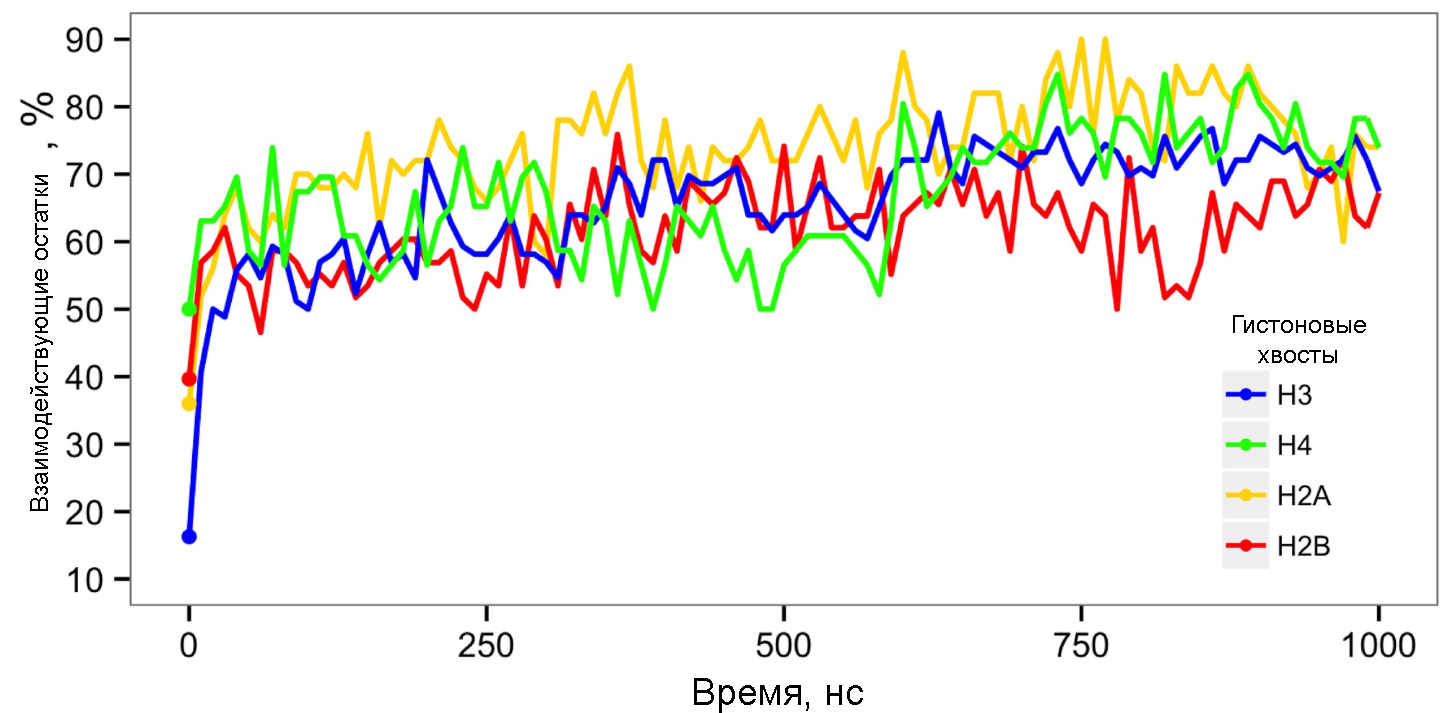
\includegraphics[width=\textwidth]{images/p2/jmb/part2_2_f4.pdf}
    \caption[Конденсация гистоновых хвостов на ДНК]{Конденсация гистоновых хвостов на ДНК. Доля остатков гистонового хвоста, которые имеют прямые или опосредованные водой взаимодействия с ДНК, представлена как функция времени моделирования. Начальные значения обозначены точками.}
    \label{fig:p2_2_f4}
\end{figure}

\begin{figure} [H]
    \centering
    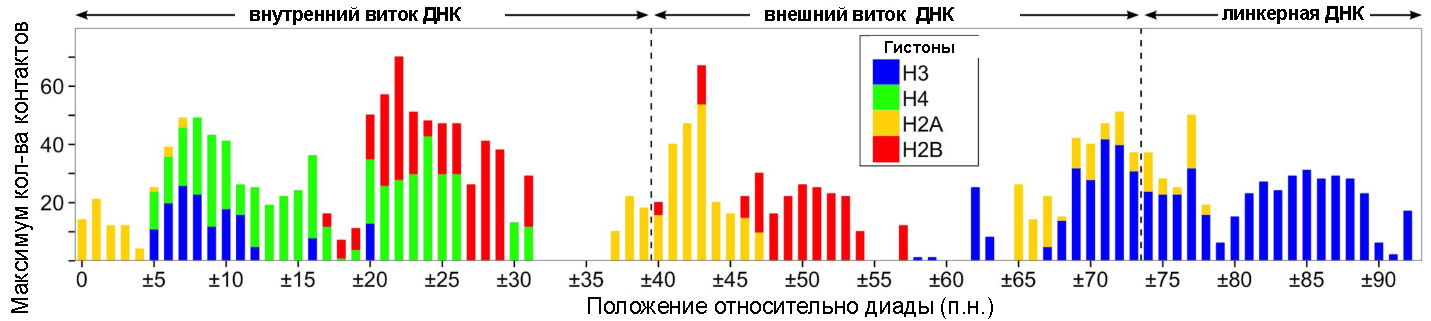
\includegraphics[width=\textwidth]{images/p2/jmb/part2_2_f5.pdf}
    \caption[Доступность ДНК для взаимодействия с гистоновыми хвостами]{Доступность ДНК для взаимодействия с гистоновыми хвостами. Максимальное количество атом-атомных контактов между ДНК и гистоновыми хвостами показано для всех кадров из различных систем моделирования (FN, FNnt и FNbb).}
    \label{fig:p2_2_f5}
\end{figure}



\subsubsection{Хвосты гистонов ``застревают’’ в малых бороздках ДНК и влияют на доступность эпигенетически модифицированных сайтов}
    Конденсация гистоновых хвостов на ДНК в ходе моделирования явно изменила конформационную динамику хвостов и самой ДНК, фактически она напоминала двумерную диффузию на поверхности ДНК с малыми бороздками ДНК, служащими кинетическими ловушками. Несмотря на обширное моделирование, за 1 мкс мы заметили, что хвосты двух копий одного и того же гистона часто исследовали не перекрывающиеся подмножества конформационного пространства. Мы предполагаем, что переключение между различными конформационными подпространствами для таких хвостов происходило во временном масштабе более длительном, чем время нашего моделирования (Рис. \ref{fig:p2_2_f6}). Такое поведение согласуется с экспериментальными данными по химическому  сшиванию и ЯМР гистоновых хвостов \cite{lee_n-terminal_1997,zhou_histone_2012}. Интересно, что в нашем микросекундном моделировании скорость конформационной динамики гистоновых хвостов зависела от их конформации и способа связывания с ДНК. Например, амплитуда колебаний хвоста H3 на одной стороне нуклеосомы, который адсорбируется на линкерной ДНК, была намного выше (из-за гибкости линкерной ДНК) по сравнению с другим хвостом H3, который был компактно свернут на около входа ДНК в нуклеосому. Динамические характеристики гистоновых хвостов в мононуклеосомах и массивах нуклеосом недавно были исследованы с помощью ряда методов, включая твердотельный ЯМР и ЯМР в растворе, дейтеро-водородный обмен \cite{kato_characterization_2009,zhou_histone_2012,gao_histone_2013}. Данные исследования содержат достаточно противоречивые выводы. Принимая во внимание наши результаты, мы предполагаем, что динамика гистоновых хвостов даже в компактных массивах нуклеосом может быть организована неоднородным образом, при этом одни хвосты стабильно свернуты, в то время как другие активно исследуют конформационное пространство.

    Подробный анализ взаимодействий между отдельными боковыми цепями аминокислот и основаниями ДНК указывает на то, что определенные боковые цепи хвостов гистонов могут быть глубоко вставлены в малые бороздки ДНК, взаимодействуя с основаниями ДНК и выступая в качестве якорей, стабилизирующих взаимодействия и ограничивающие конформационную динамику. Наибольшее количество контактов с основаниями ДНК образовано аргининами и лизинами, расположенными внутри гистоновых хвостов. А именно, в основной (FN) модели, следующие остатки показали высокую склонность к взаимодействию с основаниями малой бороздки ДНК: R8 и R26 гистона H3; K16 и R17 гистона H4; R11, K13 и K126 гистона H2A, R29 и R30 гистона H2B. Интересно, что для хвостов H3 и H4 ни одно из этих взаимодействий с основаниями ДНК не наблюдалось в исходной рентгеновской структуре. В то время, как среди контактов белок-ДНК внутри гистонового кора преобладали взаимодействия с фосфатами (в модели FN 82\% - фосфаты, 16\% - сахара, 2\% - основания), в области гистоновых хвостов 17\% контактов - это взаимодействия с основаниями, что значительно больше, чем  количество контактов между основаниями ДНК и гистонами в кристаллической структуре (8\%).

    Следует отметить, что многие упомянутые выше сайты потенциально могут подвергаться посттрансляционным модификациям, включая метилирование аргининов и метилирование и ацетилирование лизинов. Например, два из наиболее важных эпигенетически модифицированных остатков на гистоне H3 (H3K9 и H3K27) расположены рядом с остатками аргинина (H3R8 и H3R26), которые показали высокую тенденцию к встраиванию в малые бороздки ДНК. Следовательно, такие мотивы аргинин-лизин внутри гистоновых хвостов могут влиять на доступность определенных лизинов для эффекторных белков и их способность посттрансляционно модифицироваться.
    
    Если мы проанализируем те сайты, которые устанавливают прямые контакты с нуклеотидами в малой бороздке ДНК в наших моделях, наиболее выраженным является H4K16, который находится в позиции ДНК SHL -1,5. Это хорошо известный сайт ацетилирования, который регулирует компактизацию хроматина и связывание ремоделера ACF \cite{shogren-knaak_histone_2006}. Исследование мононуклеосом методом ЯМР подтвердило гибкость остатков 1-15 хвоста гистона H4, тогда как остатки 16-22 плотно взаимодействуют с нуклеосомным кором и не демонстрируют мобильности в соответствующей шкале времени ЯМР. Более того, было экспериментально подтверждено, что ацетилирование, имитирующее мутацию H4K16Q, которая, согласно нашему исследованию, вероятно, ослабит взаимодействие этого остатка с малой бороздкой ДНК из-за потери положительного заряда боковой цепи, вызывает структурное разупорядочение в этой области \cite{zhou_histone_2012}. В соответствии с нашими наблюдениями, экспериментальное исследование показало, что H4H18 и H4K16 могут быть связаны с позициями ДНК SHL $\pm$1.5 \cite{weng_probing_2014}. Наши наблюдения о связывании малой бороздки с H4K16 также согласуются с более ранними выводами Erler et al. в REMD-моделировании нуклеосом \cite{erler_role_2014}. Совсем недавно Collepardo-Guevara et al. в многомасштабном моделировании показали, что ацетилирование лизина увеличивает содержание вторичных структур в гистоновом хвосте и снижает доступность хвоста для решающих межнуклеосомных взаимодействий, компактизующих хроматиновые волокна \cite{collepardo-guevara_chromatin_2015}, что согласуется с более ранним моделированием конформационного ансамбля фрагментов гистоновых хвостов без ДНК в растворе \cite{potoyan_energy_2011,potoyan_regulation_2012}. Эти результаты также согласуются с более ранней работой по моделированию взаимодействий ДНК с пептидами из H4-хвоста \cite{korolev_h4_2007,korolev_molecular_2014}, в которой авторы предположили, что заряженные группы аргининов и лизинов играют главную роль в притяжении ДНК-ДНК через хвост гистона, образуя мосты между фосфатными группами и взаимодействую с электроотрицательными участками в малой бороздке.

    Наш сравнительный анализ взаимодействий гистонов с ДНК в различных областях нуклеосомы предполагает, что большинство взаимодействий в области глобулярных частей гистонов обеспечивается преимущественно остатками аргинина, в то время как взаимодействия между хвостами гистонов и ДНК почти в равной степени обеспечиваются остатками аргинина и лизина (Рис. \ref{fig:p2_2_f7}). Это не относится к исходной конформации, происходящей из кристаллической структуры NCP, где взаимодействия белок-ДНК через остатки лизина в значительной степени недостаточно представлены. Хотя следует отметить, что в кристаллической структуре NCP дополнительные контакты гистон-ДНК могут формироваться с соседними нуклеосомами в кристаллической решетке, которые мы не включаем в наш анализ. Такая тенденция согласуется со склонностью аргининов находится в малых бороздках ДНК, как это наблюдалось в кристаллических структурах многих комплексов белок-ДНК \cite{rohs_role_2009}. Как видно из рисунка \ref{fig:p2_2_f7}, глицин также преобладает в H3, H2A и особенно в N-концевых хвостах H4, и его карбонильная группа основной цепи может образовывать неспецифические контакты с фосфатами основной цепи ДНК. Важно отметить, что, хотя прямые контакты белков с основаниями ДНК (прямое считывание) обычно считаются почти отсутствующими в нуклеосомах и не влияют на позиционирование нуклеосом, это может быть слишком упрощенной картиной. Например, было показано, что гистоновые хвосты могут вносить вклад в зависимое от последовательности позиционирование нуклеосом \cite{yang_core_2007}. Однако этот эффект не воспроизводился на последовательностях с высоким сродством. Обширные контакты гистоновых хвостов с основаниями ДНК, наблюдаемые в нашем исследовании, могут помочь понять и интерпретировать эти экспериментальные результаты.

\subsubsection{Выпячивание ДНК возле точек входа/выхода модулируется конформациями гистонового хвоста}
    Теперь обратим внимание на анализ связи между конформацией гистоновых хвостов и геометрией нуклеосомной ДНК. В ходе моделирования проявились некоторые изменения в конформации ДНК (Рис. \ref{fig:p2_2_f3}aб). Самая большая замеченная перестройка -- выпячивание ДНК рядом с ее точкой входа в нуклеосому в районе SHL $\pm$6,5. Данную перестройку можно было наблюдать только во временных масштабах более 100 нс, и она была обусловлена различными конформациями гистоновых хвостов (Рисунок \ref{fig:p2_2_f6}). Взаимодействия в этой области ДНК (концевые 10 п.н. коровой ДНК) в основном представлены взаимодействиями с гистоновыми хвостами, а не с глобулярными доменами, что позволяет предположить, что гистоновые хвосты могут оказывать сильное влияние на конформацию ДНК, приводя к потенциальной стабилизации или дестабилизации всей нуклеосомы. Действительно, в моделировании FN-модели терминальная коровая область ДНК вокруг SHL +6,5 образовывала намного больше контактов с гистоновыми хвостами, чем ее симметричный аналог в SHL -6,5 (184 контакта против 64), что вызывало ее стабилизацию и предотвращало выпячивание ДНК. Эта стабилизация, по-видимому, была вызвана обширными взаимодействиями с N-концевым хвостом H3, который формирует компактную вторичную структуру около места входа / выхода ДНК, а также вставкой H2A K126 в малую бороздку ДНК (Рис. \ref{fig:p2_2_f6}). Таким образом С-концевой хвост H2A также может участвовать в стабилизации ДНК. Фактически, недавно было экспериментально обнаружено, что частичная делеция С-концевой области H2A приводит к разворачиванию последних 10 п.н. коровой ДНК \cite{shukla_docking_2011}. В соответствии с этим фактом, колебания концевых частей коровой ДНК были менее ограниченными в нашем моделировании для системы NCPm, которая имела усеченные гистоновые хвосты (Рис. \ref{fig:p2_2_f3}aб).


\begin{figure} [H]
    \centering
    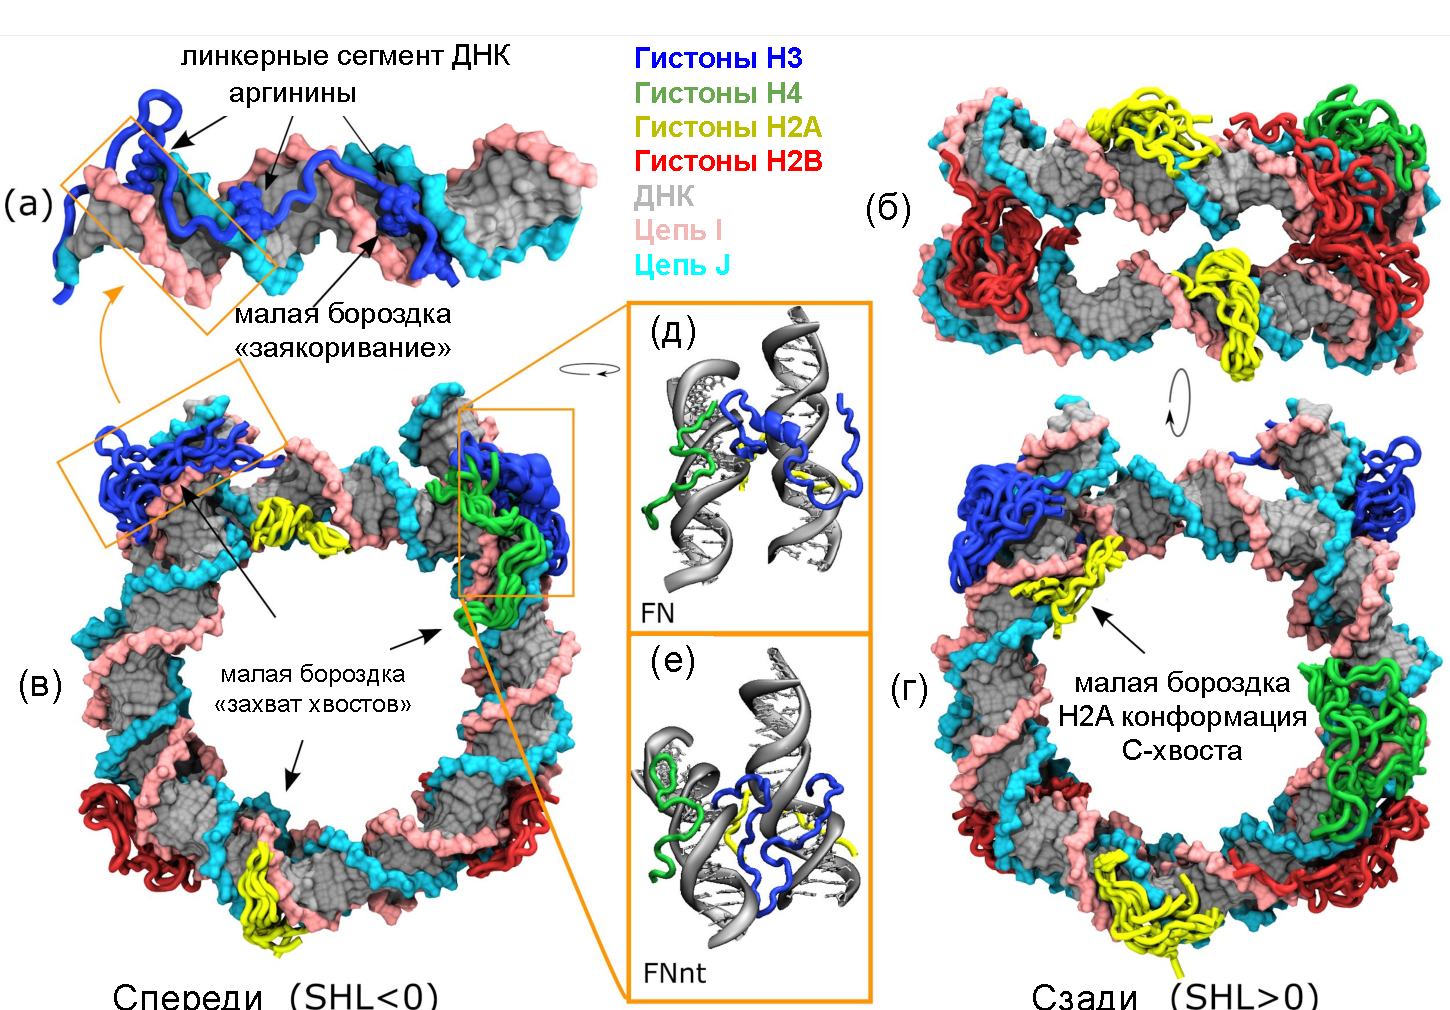
\includegraphics[width=\textwidth]{images/p2/jmb/part2_2_f6.pdf}
    \caption[Типичные паттерны взаимодействия гистоновых хвостов с ДНК]{Типичные паттерны взаимодействия гистоновых хвостов с ДНК, наблюдаемые при МД моделировании. (а) Типичная конформация N-концевого хвоста H3, взаимодействующего с линкерной ДНК. (б) - снизу, (в) - спереди и (г) - виды нуклеосомы с множественными наложенными конформациями гистонового хвоста, наблюдаемыми в течение 1 мкс МД моделирования (изображены каждые 100 нс с отброшенными первыми кадрами 250 нс). (д) формирование $\alpha$-спирали, образованной остатками 21-28 одного из хвостов H3 (цепь A), (е) альтернативное стабильное положение хвоста H3, ``состыкованное'' между супервитками ДНК.}
    \label{fig:p2_2_f6}
\end{figure}

\begin{figure} [H]
    \centering
    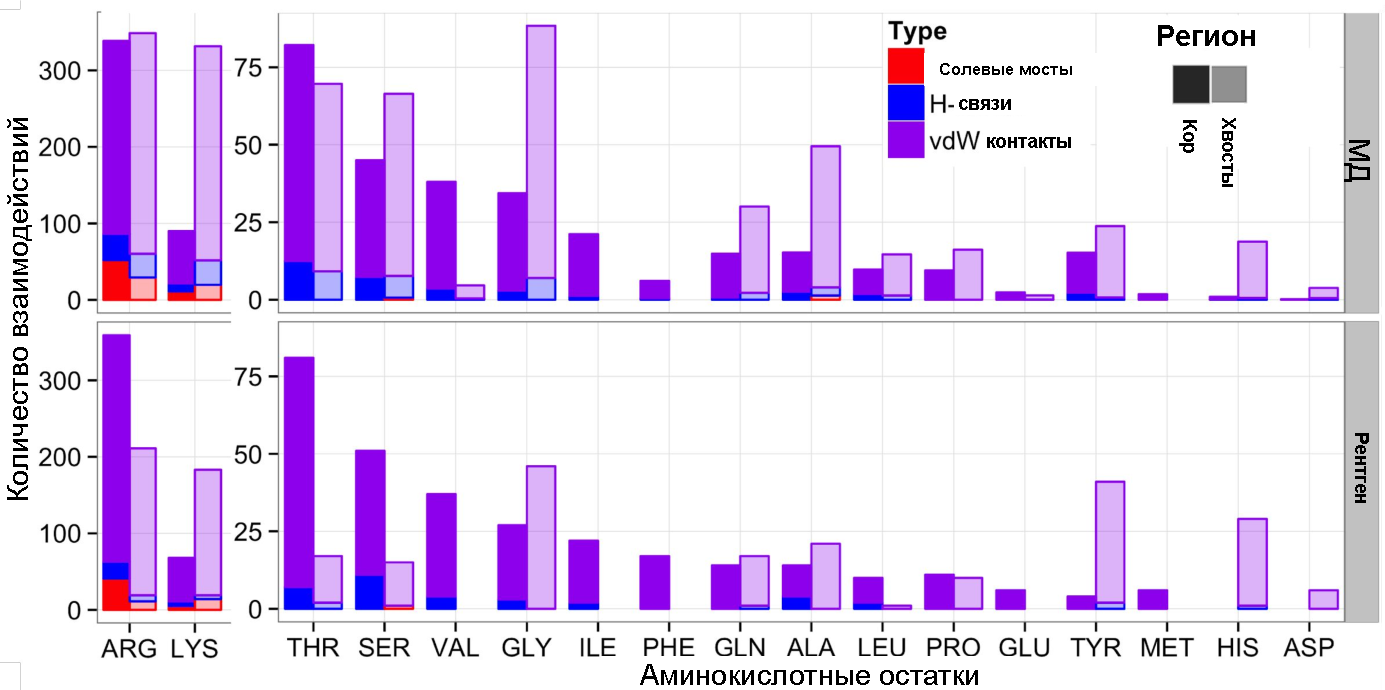
\includegraphics[width=\textwidth]{images/p2/jmb/part2_2_f7.pdf}
    \caption[Взаимодействия белок-ДНК в нуклеосоме]{Количественная оценка взаимодействий белок-ДНК по типу, участку гистона и участвующим аминокислотам.}
    \label{fig:p2_2_f7}
\end{figure}

\begin{figure} [H]
    \centering
    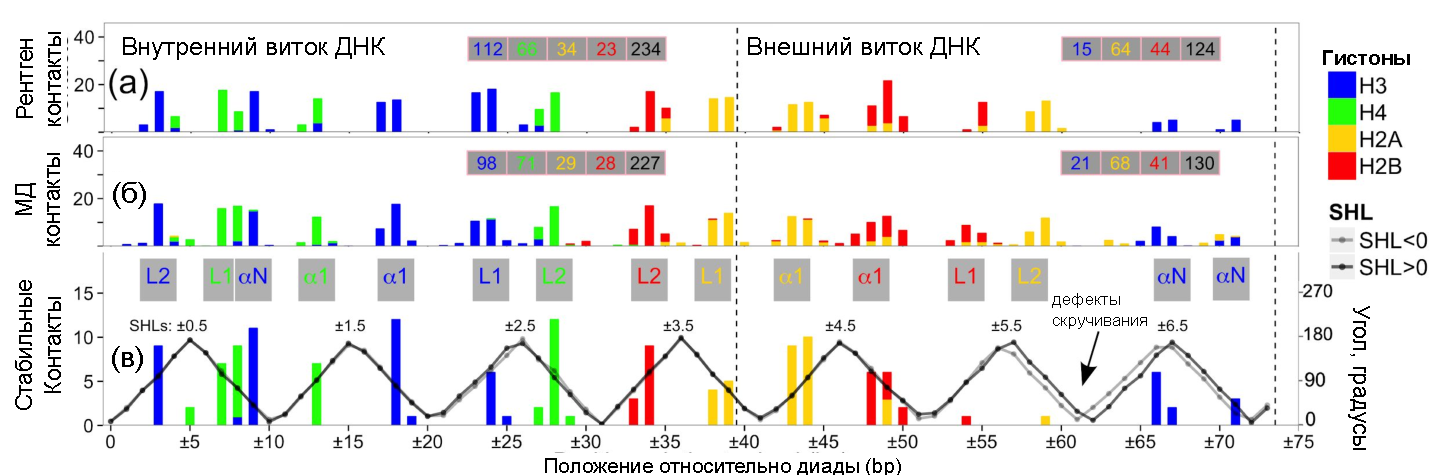
\includegraphics[width=\textwidth]{images/p2/jmb/part2_2_f8.pdf}
    \caption[Взаимодействия белок-ДНК в области нуклеосомного кора]{Взаимодействия белок-ДНК в области нуклеосомного кора. (а) Профиль контактов для рентгеновской структуры, усредненный по двум половинам нуклеосомы. (б) Среднее количество контактов по всем кадрам и по симметричным половинам нуклеосомы. Общее количество контактов для соответствующих участков ДНК и гистонов показано в розовых рамках для графиков (а) и (б). (в) Количество стабильных контактов белок-ДНК. В каждой позиции ДНК указывается количество уникальных стабильных контактов атом-атом, наблюдаемых на любой половине нуклеосомы (т.е. связанные с симметрией стабильные контакты, наблюдаемые в двух половинах нуклеосомы, подсчитывались только один раз, асимметричные контакты вносились индивидуально). Структурные элементы сайтов связывания ДНК аннотированы в верхней части этого графика разными цветами, соответствующими разным типам гистонов. Черные и серые кривые показывают периодичность вращения ДНК в структуре нуклеосом, усредненной по траектории.}
    \label{fig:p2_2_f8}
\end{figure}





\subsubsection{Сайты связывания ДНК в гистоновом коре демонстрируют возможность перестройки, сопровождающейся образованием дефектов кручения ДНК}
    В наших предыдущих разделах мы говорили о взаимодействиях между гистоновыми хвостами и ДНК; в этом разделе мы обсудим взаимодействия гистонов с ДНК, вовлекающие глобулярные домены гистонов, и их связь с перестройками геометрии ДНК. Из анализа кристаллической структуры NCP известно, что ДНК имеет семь пар симметричных сайтов связывания, где малая бороздка ДНК обращена к октамеру гистонов. В каждом сайте связывания ключевой аргинин вставлен в малую бороздку в большинстве случаев, за исключением канонических аргининов R49 из обеих копий H3, которые расположены слишком далеко, чтобы их можно было вставить в малую бороздку в районе SHL $\pm$6.5. В то же время это место имеет небольшое количество контактов с гистоновым ядром (Рис. \ref{fig:p2_2_f8}а,б). Наш анализ динамики взаимодействий гистон-ДНК показал, что этот канонический H3R49 действительно может быть вставлен в соответствующую малую бороздку из-за выпячивания ДНК в районе SHL $\pm$6.5, описанной ранее. Этому выпячиванию, по-видимому, способствовало образование дополнительных и перестройка существующих контактов между $\alpha$N-спиралью H3 и ДНК. Чтобы понять последствия этих изменений для общей геометрии ДНК, мы построили график эффективного вращения пар оснований ДНК относительно положения суперспиральной оси (Рис. \ref{fig:p2_2_f8}в). Мы наблюдали сдвиг в общем скручивании ДНК на одну пару оснований вокруг SHL -6/-6,5, а в случае модели NCPm такие сдвиги наблюдались в области от SHL -5,5 до конца коровой ДНК. Подобные сдвиги в геометрии скручивания ДНК ранее были названы ``твист-дефектами'' \cite{edayathumangalam_nucleosomes_2005}. Некоторые экспериментальные исследования показали, что нуклеосома существует в растворе как смесь различных состояний твист-дефектов, и только некоторые из них могут быть увидены в кристаллических структурах путем изменения основной последовательности ДНК, ее длины или добавления интеркалирующих агентов \cite{edayathumangalam_nucleosomes_2005}. В нашем исследовании мы впервые смогли наблюдать образование таких дефектов \textit{in silico} и описать атомистические детали, лежащие в основе связи между геометрией ДНК и взаимодействиями гистон-ДНК.
    
    Чтобы выяснить закономерности взаимодействий в различных сайтах связывания гистонов с ДНК, мы вычислили количество так называемых стабильных контактов (см. Методы). Как видно на рисунках \ref{fig:p2_2_f8}a-в, количество контактов между гистоновым кором и внутренним супервитком ДНК было почти вдвое больше, чем количество контактов с внешним витком ДНК. Это согласуется с более легким разворачиванием внешнего витка ДНК в экспериментах с единичными молекулами \cite{hall_high_2009,brower-toland_mechanical_2002}. Более того, рисунок \ref{fig:p2_2_f8} показывает четкую иерархию между различными каноническими сайтами связывания. Сайты связывания вокруг SHL $\pm$0,5 и SHL $\pm$4,5 имеют наибольшее количество динамически стабильных контактов в соответствии с картированием с высоким разрешением взаимодействий белок-ДНК в нуклеосомах, полученным путем механического растягивания ДНК. Последние эксперименты показали, что наиболее сильные взаимодействия гистон-ДНК происходят вокруг диады и в районе расположения $\pm$40 пар оснований от диады \cite{hall_high_2009}.
    
    Первый сайт связывания гистонов с ДНК вокруг SHL $\pm$0,5 образован петлями L1/L2 димера H3-H4, с дополнительным взаимодействием, исходящим от N-конца $\alpha$N-спирали H3, что делает этот сайт очень особенным с точки зрения его уникальной специфической организации. Различия между паттернами связывания гистонов с ДНК наблюдались на картах нуклеосом по всему геному, и недавно с помощью геномного анализа позиционирования нуклеосом был обнаружен необычный сигнал относительно содержания A|T/G|C в нуклеосомной ДНК в девяти парах оснований от центра нуклеосомы \cite{brogaard_map_2012}. Предполагалось, что это может быть связано с внедрением H3R40 глубоко в малую бороздку ДНК, либо с образованием специфичных для последовательности контактов с основаниями \cite{davey_does_2013}. Однако мы не наблюдали таких контактов в микросекундном масштабе времени, и H3R40 взаимодействовал с фосфатами ДНК, а не с основаниями.
    
    Второй высокостабильный сайт связывания вокруг SHL $\pm$4.5 образован двумя $\alpha$1-спиралями димера H2A-H2B, тогда как сайты связывания ДНК с наименьшим числом стабильных взаимодействий локализованы на SHL $\pm$6.5, SHL $\pm$5.5 и SHL $\pm$1.5. Карта контактов гистонов с ДНК согласуется с профилем флуктуаций ДНК (Рис. \ref{fig:p2_2_f9}), а флуктуации ДНК показывают видимое увеличение при SHL $\pm$1,5. Это согласуется с повышенной конформационной гибкостью ДНК в этих сайтах при связывании малых молекул или белков показанной в недавних экспериментах. Эти эксперименты показали, что SHL $\pm$1,5 является местом связывания ионов тяжелых металлов и интеркалирующих противоопухолевых агентов \cite{tan_nucleosome_2011}. Отсутствие стабильных взаимодействий вокруг SHL $\pm$5.5/$\pm$6.5 также соответствует увеличению флуктуаций ДНК. Колебания на самом конце коровой ДНК несколько меньше, что объясняется их стабилизацией через N- и С-концевые хвосты H3 (см. Предыдущие разделы). Малая стабильность и высокая гибкость сайтов связывания SHL $\pm$5.5 и SHL $\pm$6.5 может указывать на то, что эти сайты вносят лишь небольшие энергетические барьеры при разворачивании ДНК из нуклеосомы. Биологически значимый процесс, который основан на таком постепенном разрыве контактов ДНК-гистонов, включает транскрипцию РНК-полимеразами, которая может происходить без вытеснения нуклеосом \cite{studitsky_mechanism_1997}. Нуклеосомный барьер для транскрипции, исследованный с помощью паттернов транскрипционного паузирования, показал, что первый барьер встречается полимеразой, когда передний край полимеразы входит в область примерно в 40 п.н. от диады \cite{jin_synergistic_2010}. Данный факт согласуется с представлением о том, что первые два сайта связывания почти не представляют барьера для транскрипции.


\begin{figure} [H]
    \centering
    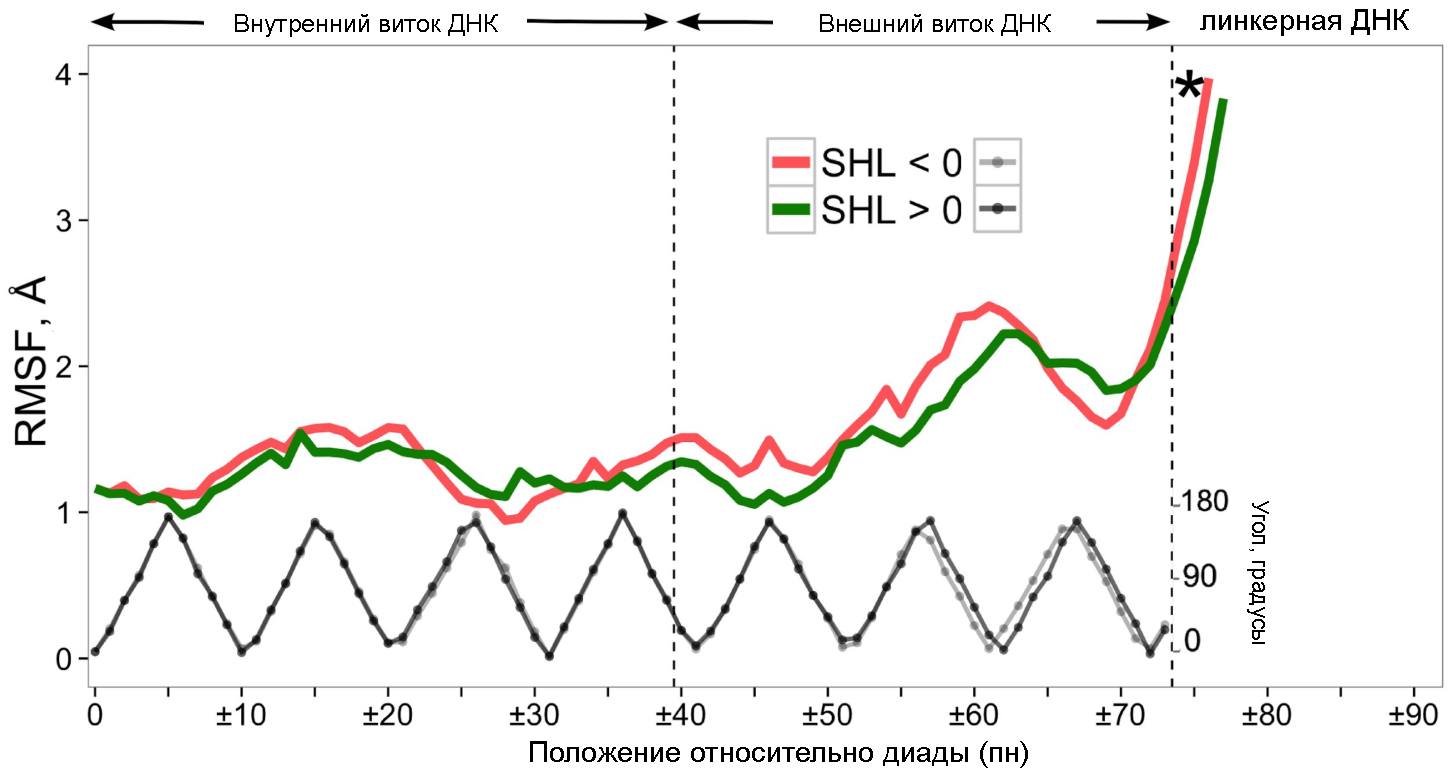
\includegraphics[width=\textwidth]{images/p2/jmb/part2_2_f9.pdf}
    \caption[Флуктуации ДНК в нуклеосоме]{Флуктуации ДНК в нуклеосоме. RMSF центров пар оснований для двух симметричных половин нуклеосом (красная и зеленая кривые); черные и серые кривые показывают периодичность вращения суперспирали ДНК. Точки данных, превышающие RMSF 4\AA, не показаны. Звездочкой обозначена та же цепь, что и на рисунке \ref{fig:p2_2_f3}.}
    \label{fig:p2_2_f9}
\end{figure}

\subsection{Обсуждение}
    В данном разделе мы представили молекулярно-динамическое исследование полной модели нуклеосомы с полноразмерными гистоновыми хвостами и линкерными участками ДНК. Мы использовали полноатомное моделирование в явном растворителе и распространили этот подход на микросекундную шкалу времени. Микросекундная шкала времени и многочисленные сравнительные симуляции позволили нам получить представление о функционально значимых перестройках в конформациях нуклеосом, включая связь между конформациями гистоновых хвостов и ДНК.

    Механистические наблюдения, полученные в нашем исследовании, предполагают, что конформационные перестройки внутри коровой ДНК зависят от паттернов взаимодействий ДНК с гистонами. В частности, мы наблюдали, что N-концевой хвост H3 и C-концевой хвост H2A устанавливают много контактов с коровой ДНК и могут стабилизировать геометрию ее концевой области, подавляя образование локализованных дефектов кручения внутри ДНК. С другой стороны, конформация хвостов, которые выступают из нуклеосомы, способствуют образованию состояний с дефектами кручения, которые могут быть важными промежуточными звеньями в скольжении и ремоделировании нуклеосом \cite{mueller-planitz_nucleosome_2013}. Мы предлагаем наличие механизма, с помощью которого наблюдаемое чрезмерное скручивание ДНК в терминальной области ДНК может представлять собой начальное состояние дефекта кручения ДНК, которое может быть стабилизировано последующими перестройками взаимодействий ДНК в центральной области гистонов. Последующее скольжение нуклеосом может происходить за счет распространения этого дефекта дальше по кору нуклеосомы. Интересно отметить, что несколько исследований по химическому сшиванию мононуклеосом \textit{in vitro} ранее показали, что гистоновые хвосты занимают различные предпочтительные конформации в NCP, нуклеосомах с линкерами и нуклеосомами с гистоном H1 \cite{lee_linker_1998,angelov_preferential_2001}. Данный факт позволяет предположить, что гистоновые хвосты очень чувствительны к наличию/отсутствию линкерной ДНК, гистона H1 и изменений в нуклеосомном окружении.
    
    В соответствии с результатами экспериментов по химическому сшиванию  ДНК с гистонами \cite{angelov_preferential_2001,stefanovsky_laser-induced_1989} мы обнаружили, что гистоновые хвосты легко адсорбируются на линкерную (в основном хвосты H3) и коровую ДНК (в основном хвосты H4, H2B и H2A), и большинство контактов гистонов с ДНК представлено контактами с гистоновыми хвостами. О возможности взаимодействия N-концевых хвостов H3 с линкерной ДНК сообщалось ранее \cite{rhee_subnucleosomal_2014,angelov_preferential_2001}. Фактически, эффективность химического сшивания в NCP оказалась в 3–4 раза ниже для H2A, H2B и H4 и в 10–12 раз ниже для H3 по сравнению с полными нуклеосомами с линкерной ДНК \cite{stefanovsky_laser-induced_1989}. Более того, наше детальное изучение поведения гистоновых хвостов показало, что их динамика в микросекундном масштабе характеризуется ограниченной диффузией на поверхности ДНК и кинетическим захватом хвостовых областей в малых бороздках ДНК. Наблюдаемое стабильное прикрепление гистоновых хвостов к коровой и линкерной ДНК предполагает глубокие последствия для взаимодействий нуклеосом с другими белками хроматина. В самом деле, когда эти белки связываются с гистоновыми хвостами или ДНК, сначала они должны проконкурировать со взаимодействиями ДНК-гистоновый хвост и вытеснить соответствующего партнера. Например, Pilotto et al. недавно экспериментально продемонстрировали элегантную практическую иллюстрацию этой концепции на примере комплекса LSD1-CoREST, который действует как деметилаза H3K4 \cite{pilotto_interplay_2015}. Было высказано предположение, что этот комплекс связывается с нуклеосомой через свою субъединицу CoREST, которая вытесняет хвост H3 с ДНК. Это смещение критически необходимо для того, чтобы сделать метилированный H3K4 доступным для взаимодействий с его субъединицей LSD1. Можно предположить, что такие механизмы могут быть использованы для организации перекрестного взаимодействия между множественными сайтами связывания на гистоновых хвостах, включая сайты ПТМ и их соответствующих партнеров по связыванию \cite{ruthenburg_multivalent_2007,nishi_crosstalk_2015}.
    
    Атомистические детали связывания гистонового хвоста с ДНК, выявленные в ходе нашего исследования, дополнительно показали, что этому процессу способствует вставка закрепляющих боковых цепей аргинина и лизина в малые бороздки ДНК. Это, в свою очередь, повлияло на те остатки, которые служат эпигенетически модифицированными сайтами в хвостах гистонов, или на остатки, расположенные рядом с ними (например, H3K9, H3K27, H4K16 и H3R8, H3R26 и т.д.). Присутствие множества сайтов связывания на одном хвосте гистонов и окклюзия боковой цепи малыми бороздками может вызывать кооперативные эффекты. А именно, связывание одного партнера с его сайтом связывания на ДНК или сайтом гистонового хвоста может вызвать смещение гистонового хвоста от ДНК и, таким образом, облегчать связывание другого партнера. Подобные эффекты могут быть вызваны посттрансляционными модификациями, такими как метилирование аргинина и особенно ацетилирование лизина, которые не способствуют встраиванию этих остатков в малую бороздку и, таким образом, могут способствовать конформационной гибкости и доступности связывания гистоновых хвостов. Наблюдаемые эффекты помогают наметить дальнейший план экспериментальных исследований, которые должны прояснить сложное динамическое взаимодействие между посттрансляционными модификациями гистонов и доступностью гистоновых хвостов для связывания эффекторных белков.

\subsection{Материалы и методы}
\subsubsection{Построение начальной модели}
    В качестве отправной точки мы использовали рентгеновскую кристаллическую структуру высокого разрешения (1,9\AA) коровой частицы нуклеосомы, образованную рекомбинантными вариантами канонических коровых гистонов \textit{X. laevis}и модифицированной $\alpha$-сателлитной ДНК человека (PDB ID 1KX5 \cite{davey_solvent_2002}). Для создания полной нуклеосомной модели с линкерными сегментами ДНК с помощью программы NAB был сконструирован прямой дуплекс B-ДНК $(AGTC)_5$ длиной 20 п.н. \cite{macke_thomas_modeling_1997}. Используемая линкерная последовательность ДНК сбалансирована по количеству гибких и жестких динуклеотидов \cite{olson_dna_1998}. Она была прикреплена к основной ДНК на обоих концах NCP. Один из хвостов гистона H3 был слегка повернут, чтобы избежать стерических столкновений с линкерной ДНК (угол $\Psi$ Lys36 был установлен на -35 градусов) (Рис. \ref{fig:p2_2_f1}a). Минималистичная модель NCP (NCPm) была получена из той же кристаллической структуры путем усечения гистоновых хвостов в сайтах, указанных на рисунке \ref{fig:p2_2_f2} треугольниками. Все модели были явно сольватированы в прямоугольной ячейке с минимальным расстоянием между растворенным веществом и границами ячейки в 20\AA, за исключением системы FNbb (таблица 1), для которой использовался порог в 100\AA. В системы добавляли ионы натрия для нейтрализации, а затем добавляли дополнительные ионы натрия и хлора в концентрации 150 мМ по отношению к объему воды, за исключением системы FN1M, где использовалась концентрация 1 М. Точная соответствующая объемная концентрация ионов была оценена непосредственно из данных моделирования. Кристаллографические молекулы воды остались в системе, а все кристаллографические ионы были удалены. Состояния протонирования аминокислот определяли на основании значений pK их растворов при нейтральном pH, остатки гистидина считали нейтральными и протонировали на $\epsilon$-азотах. Модель FNnt была идентична модели FN, но имела нейтрально заряженные белковые концы для изучения устойчивости МД-моделирования к небольшим возмущениям. Структуры исходных моделей представлены на рис. \ref{fig:p2_2_f1}а. На выбор NaCl в качестве соли для нашего моделирования повлияло его обычное использование в экспериментах с нуклеосомами \textit{in vitro}, а также в протоколах сборки нуклеосом \cite{dyer_reconstitution_2004}.

\subsubsection{Протоколы моделирования и выбор силового поля}
    Силовое поле CHARMM36 использовалось для ДНК и белка \cite{best_optimization_2012,hart_optimization_2012}, параметры TIP3P для молекул воды и скорректированные параметры  Луо и Ру для ионов \cite{luo_simulation_2010}. Выбор силового поля всегда является деликатным вопросом из-за известных и неизвестных приближений, используемых в силовом поле, а также постоянными усилиями по улучшению силового поля, предпринимаемых разработчиками. В случае нуклеосом проблема осложняется необходимостью сочетать точные модели белков и ДНК, а также обеспечивать реалистичное моделирование взаимодействий с растворителем. Ниже мы кратко обсудим несколько недавних современных исследований о поведении различных силовых полей при моделировании нуклеосом.
    
    Точность силового поля белка, по-видимому, особенно важна для моделирования поведения изначально неупорядоченных гистоновых хвостов. Систематические исследования биомолекулярных силовых полей \cite{lindorff-larsen_systematic_2012} показали, что определенные силовые поля (например, CHARMM27, AMBER ff03) сверхстабилизируют спиральную конформацию пептидов, и поэтому эта проблема была решена в пересмотре силового поля для белков CHARMM36 \cite{best_optimization_2012}. Кроме того, несколько недавних исследований поставили под сомнение применимость силовых полей белков для специфического моделирования гистоновых хвостов \cite{erler_role_2014,collepardo-guevara_chromatin_2015,potoyan_energy_2011}. Например, Erler et al. показали, что разные версии силовых полей AMBER могут приводить к разному динамическому поведению гистоновых хвостов \cite{erler_role_2014}. Collepardo-Guevara et al. сравнили результаты моделирования с использованием современных силовых полей, включая CHARMM36, с данными ЯМР по динамике гистонового хвоста и пришли к выводу, что все силовые поля дают почти идентичные результаты \cite{collepardo-guevara_chromatin_2015}.

    Силовое поле ДНК необходимо для правильного воспроизведения конформационных переходов ДНК при моделировании нуклеосом. Параметризация силовых полей нуклеиновых кислот оказывается более сложной задачей, чем аналогичная задача для белков. В настоящее время известно, что силовые поля как CHARMM, так и AMBER воспроизводят стабильную динамику ДНК в микросекундном масштабе времени и за его пределами \cite{galindo-murillo_convergence_2015}. Однако точное воспроизведение экспериментальных результатов по зависимой  деформируемости ДНК от последовательности с использованием доступных силовых полей все еще остается нерешенной проблемой \cite{perez_frontiers_2012}.
    
    Наши модельные системы были подготовлены с помощью программы VMD \cite{humphrey_vmd_1996}, а моделирование МД было выполнено с помощью пакета NAMD 2.9 \cite{phillips_scalable_2005}. Для моделирования при постоянной температуре использовался подход динамики Ланжевена с шагом интегрирования 2 фс, параметром демпфирования 0,5 $пс^{-1}$ и T = 310K. Поддержание давления в 1 атм было реализовано методом Ланжевена. Моделирование проводилось с жесткими ковалентными связями, и ван-дер-ваальсовы взаимодействия постепенно выключались на расстоянии от 10 до 12\AA. В электростатических расчетах использовался метод PME с шагом сетки 1\AA, кубической интерполяцией, отсечкой в реальном пространстве 12\AA и параметром толерантности $10^{-6}$. Использовались периодические граничные условия. Для устранения диффузии нуклеосом к атомам C-$\alpha$ гистоновых фолдов H3 (номера остатков 64-78, 86-114, 121-131) применялись небольшие позиционные ограничения в 0,003 ккал/моль/$A^2$. Чтобы избежать расплетания пар оснований на концах ДНК в моделировании NCPm, использовали ограничивающий потенциал в виде искусственной стенки, чтобы сохранить расстояние между центрами масс оснований в концевых парах оснований в пределах 120\% от начального.

    Все системы были подвергнуты минимизации энергии и первоначальному уравновешиванию. Затем проводилось моделирование до времени моделирования 1 $\mu$с. Кадры траектории сохранялись каждые 100 пс. Мы запускали расчеты параллельно на высокопроизводительных компьютерных кластерах/суперкомпьютерах, используя эффективное распараллеливание, доступное в NAMD. Скорость моделирования варьировалась в зависимости от моделируемой системы, количества процессоров и архитектуры машины. Для справки: система модели FN моделировалась параллельно на 384 ядрах ЦП в течение 120 дней со скоростью $\sim$8 нс/день.
%21 страница

\subsubsection{Анализ траекторий}
    Анализ и визуализация траектории выполнялись с использованием набора библиотек и скриптов собственной разработки, написанных на TCL, Python и R, которые использовали возможности VMD \cite{humphrey_vmd_1996} и 3DNA \cite{lu_3dna_2008} для общего и специфического анализа структуры ДНК. Для структурного анализа нуклеосом отдельные кадры траектории были наложены на исходную кристаллическую структуру, путем минимизации значения среднеквадратичного отклонения (RMSD) между положениями атомов C-$\alpha$ спиралей гистоновых фолдов. Анализ конформации ДНК проводили по отношению к нуклеосомной суперспиральной системе отсчета, определяемой ее диадной осью и суперспиральной осью. Периодичность вращения ДНК в нуклеосоме определяли путем расчета угла между вектором пары оснований (соединяющим атомы N1 и N9 соседних оснований в паре оснований) и суперспиральной осью нуклеосомы. Максимумы и минимумы значений периодичности вращения соответствовали целочисленным и полуцелым значениям SHL.
    
    Подробный анализ взаимодействий гистонов с ДНК проводился для каждого кадра траектории (первые кадры 250 нс не учитывались как начальный период конформационного уравновешивания) путем анализа положений соответствующих атомов. Контакты (SC) между двумя атомами гистона и ДНК определялись как контакты между тяжелыми атомами на расстоянии менее 3,9\AA. Контакты были дополнительно классифицированы следующим образом: солевые мостики (SB) включают два заряженных неводородных атома на расстоянии менее 3,9\AA; водородные связи (HB) были определены как связи между донорными (D) и акцепторными (A) атомами с водородом между ними (DH-A), где расстояние между D и A было меньше 3,5\AA, а DH-A угол составлял больше 150 градусов; контакты Ван-дер-Ваальса (vdW) были определены как контакты между атомами, которые не были связаны водородными связями и не образовывали солевой мостик; и опосредованные водой взаимодействия (WM) определялись как взаимодействия между неводородными атомами ДНК или гистонами, которые образуют водородную связь с одной и той же молекулой воды. Мы также ввели понятие стабильных контактов между ДНК и белком, чтобы описать контакты, которые сохранялись во время моделирования. А именно, они были определены как отдельные пары атомных контактов между ДНК и молекулами белка, которые присутствовали более чем в 80\% кадров траектории после начального периода конформационного уравновешивания.

\subsubsection{Соглашения об описании структуры нуклеосом}
    Позиции пар оснований ДНК были пронумерованы относительно центральной пары оснований (называемой диадой), ее положение принималось равным нулю. Вращательная ориентация двойной спирали ДНК полуколичественно описывается параметром сверхспирального расположения (SHL) (Рис. \ref{fig:p2_2_f1}a), который мы расширяем, чтобы включить не только коровую ДНК (SHL от 0 до $\pm$7), но и линкерную ДНК (SHL до $\pm$9). Исходные 147 пар оснований ДНК NCP называются ``коровой ДНК'', а области, где коровая ДНК соединяется с линкерной ДНК, называются сайтами входа/выхода ДНК. Мы различаем две части в каждом гистоне: область хвоста (как указано на рисунке \ref{fig:p2_2_f2}) и остальную часть, называемую глобулярной частью гистона. Ключевыми элементами глобулярных областей являются спирали гистоновых фолдов $\alpha$1, $\alpha$2 и $\alpha$3 \cite{baxevanis_variety_1995} и петли L1, L2, как показано на рисунке \ref{fig:p2_2_f2}.


\subsubsection{Благодарности}
Исследования данного раздела были поддержаны программами внутренних исследований Национальной медицинской библиотеки и Национального института рака, Национальных институтов здоровья; и Российским научным фондом [грант № 14-24-00031] (разработка алгоритмов визуализации нуклеосом). Автор был поддержан программой сотрудничества между США и Россией в области биомедицинских наук. В этом исследовании использовались высокопроизводительные вычислительные возможности кластера Biowulf Linux в Национальном институте здравоохранения, Бетесда, Мэриленд \url{http://biowulf.nih.gov}. Данное исследование было частично поддержано Суперкомпьютерным центром МГУ им. М.В. Ломоносова и вычислительными ресурсами суперкомпьютера Hexagon Cray XE6m-200, в университете Бергена и норвежском метацентре высокопроизводительных вычислений (NOTUR).










\section{Моделирование коровых частиц нуклеосом на масштабах свыше 10 микросекунд}
\textit{Данный раздел описывает работы, выполненные в 2017-2020 годах, являющиеся продолжением работ предыдущего раздела. Работы основаны на использовании более современных компьютерных архитектур с использованием графических процессоров и учитывают серьезный объем новых экспериментальных данных, опубликованных в 2017-2020 годах. Интерактивные материалы раздела доступны по ссылке} \url{http://intbio.github.io/nucl_MD_15mus/}.

% новая статья
\subsection{Введение}
Многие химические и физические сигналы регулируют обработку генетической информации в живых клетках.
У эукариот эта регуляция в основном происходит на уровне нуклеосом - последовательных отрезков ДНК, обернутых вокруг октамеров гистоновых белков \cite{kornberg_chromatin_1974,olins_spheroid_1974}. Четыре типа гистонов (H3, H4, H2A, H2B) образуют два типа димеров (H3-H4, H2A-H2B). Четыре димера образуют октамер с двойной осью симметрии (диадной осью) \cite{burlingame_crystallographic_1985}. Как известно из кристаллографических исследований, примерно 147 пар оснований ДНК резко изгибаются вокруг октамера в $\sim$1,7 витка левой суперспирали, формируя коровую частицу нуклеосомы (NCP) \cite{luger_crystal_1997} (Рис. \ref{fig:p2_3:f1}а).

При формировании нуклеосом жесткая макромолекула ДНК с персистентной длиной около 50 нм должна резко изгибаться до радиуса кривизны всего в 5 нм. Это возможно благодаря электростатическому взаимодействию отрицательно заряженной ДНК с положительно заряженными гистонами, дополненному индивидуализированным паттерном взаимодействия белок-ДНК на атомном уровне в 14 сайтах связывания ДНК (по 7 с каждой стороны NCP). Эти сайты связывания расположены в положениях, где малая бороздка ДНК обращена к поверхности октамера и обычно присутствует боковую цепь остатка аргинина, которая выступает в пространство малой бороздки. Общая энергия взаимодействий гистонов с ДНК в нуклеосомах оценивается как не менее 23 ккал/моль \cite{onufriev_nucleosome:_2019}.
Стабильность нуклеосом может варьироваться на 2-4 ккал/моль в зависимости от гибкости последовательности ДНК \cite{thastrom_sequence_1999}, которая, как было показано, зависит от содержания GC, наличия гибких динуклеотидных ступеней YR, участков поли (dA:dT), эпигенетических модификации оснований ДНК, таких как 5-метилцитозин и т. д. \cite{ngo_asymmetric_2015,chua_mechanics_2012,zhurkin_sequence-dependent_1985,segal_genomic_2006}. Еще одним важным фактором являются вариации последовательности гистонов. Несмотря на то, что гистоновые белки одни из самых консервативных белков в эволюционном смысле, они подвержены множеству функционально значимых вариаций, включая посттрансляционные модификации (ПТМ) \cite{zhao_comprehensive_2015} и изменение последовательности за счет включения вариантов, изоформ и мутаций гистонов \cite{draizen_histonedb_2016,singh_replication-dependent_2018,nacev_expanding_2019}.

Представление о нуклеосомах как о средстве простой компактизации ДНК теперь устарело.
% Благодаря своей роли в обеспечении доступа к ДНК, нуклеосомы играют ключевую роль в эпигенетической регуляции экспрессии генов.
Различные режимы АТФ-зависимой и АТФ-независимой динамики нуклеосом, модулируемые гистоновым составом и последовательностью ДНК, обеспечивают богатый динамический ландшафт для регуляции генома \cite{armeev_linking_2019}. Например, скольжение нуклеосом с помощью АТФ-зависимых ремоделеров хроматина \cite{paul_regulation_2018} или их реконфигурация с помощью РНК-полимераз \cite{kujirai_transcription_2020,gaykalova_structural_2015} в значительной степени вовлечены в транскрипцию и ее регуляцию. Пассивная динамика нуклеосом также участвует во многих процессах. Новаторские эксперименты Джона Видома показали, что временное отворачивание ДНК от октамера гистонов может быть использовано факторами транскрипции для доступа к их сайтам связывания \cite{li_rapid_2005}. Недавние исследования методами FRET \cite{gansen_high_2018,sabantsev_direct_2019}, ЯМР \cite{sinha_distortion_2017, kitevski-leblanc_investigating_2018}, крио-ЭМ \cite{li_mechanism_2019,bilokapic_structural_2018} и масс-спектрометрии\cite{hada_histone_2019,sanulli_hp1_2019,sinha_distortion_2017} свидетельствуют о том, что существуют более тонкие режимы конформационной динамики нуклеосом, которые воспринимаются и используются белками хроматина. Например, кручение ДНК внутри NCP обеспечивает путь для АТФ-зависимого ремоделирования нуклеосом \cite{bowman_remodeling_2019,li_mechanism_2019}. Внутренняя динамика (пластичность) гистонового ядра также участвует в этом процессе (хотя на этот счет и ведутся дискуссии) \cite{sinha_distortion_2017,yan_structures_2019,armache_cryo-em_2019}. Сообщалось, что подавление этой динамики путем введения сайт-специфичных дисульфидных сшивок в отдельные димеры H3-H4 ингибирует передвижение нуклеосом ремоделером SNF2h, увеличивает вытеснение октамера комплексом RSC \cite{sinha_distortion_2017}, блокирует термически индуцированную диффузию нуклеосом вдоль ДНК \cite{bilokapic_structural_2018} и даже нарушает компактизацию хроматина белком HP1 \cite{sanulli_hp1_2019}. Эти результаты свидетельствуют о том, что октамер гистонов может принимать конформации, альтернативные тем, которые наблюдаются в рентгеновских структурах. Действительно, используя передовые методы крио-ЭМ, Bilokapic et al. недавно наблюдали некоторые альтернативные конформации нуклеосом с развернутой ДНК, наклоненными гистоновыми $\alpha$-спиралями и общей сжатой формой NCP \cite{bilokapic_structural_2018,bilokapic_histone_2018}. Еще большие внутренние флуктуации в структуре октамера гистонов предполагают эксперименты по химической сшивке лизинов \cite{hada_histone_2019} и эксперименты FRET с высоким разрешением\cite{gansen_high_2018}.


Эти и другие исследования подчеркнули существование нового уровня динамической сложности нуклеосом, связанного с атомистическими деталями структуры. Однако структурная интерпретация этих результатов все еще остается не вполне ясной. \textit{In silico} подходы, такие как моделирование методом молекулярной динамики (МД), являются мощными инструментами, которые могут дополнять экспериментальные методы и помочь механистически интерпретировать экспериментальные результаты с высоким уровнем детализации. До сих пор моделирование с помощью МД применялось для изучения распределения ионов вокруг нуклеосом и их гидратации \cite{materese_counterion_2009}, деталей разворачивания ДНК, скольжения и разборки нуклеосом \cite{ettig_dissecting_2011, rychkov_partially_2017, zhang_exploring_2016, winogradoff_molecular_2019,brandani_dna_2018,lequieu_silico_2017}, динамики гистоновых хвостов\cite{erler_role_2014, shaytan_coupling_2016,chakraborty_molecular_2018,morrison_conformation_2018}, эффектов посттрансляционных модификаций гистонов \cite{fenley_modulation_2018,li_investigating_2018,rajagopalan_structural_2017} и их вариантов \cite{bowerman_unique_2019}, эффектов влияния последовательности ДНК \cite{sun_tmb_2019} на динамику нуклеосом, взаимодействия между олигонуклеосомами \cite{collepardo-guevara_chromatin_2015} и гистоном H1 \cite{ozturk_chromatosome_2020,perisic_sensitive_2019} и т. д. Из-за вычислительной сложности такого рода расчетов часто прибегают к упрощениям (например, удаляют гистоновые хвосты, используют неявные модели растворителя или крупно-зернистое представление молекулярной системы), либо ограничивают временные рамки моделирования. В настоящее время наиболее известные МД исследования нуклеосом в полноатомном приближении были ограничены несколькими микросекундами времени моделирования \cite{winogradoff_molecular_2019,chakraborty_molecular_2018} даже с применением специализированных суперкомпьютеров, таких как ANTON. Однако предполагается, что важные функциональные переходы в структуре нуклеосом происходят в масштабе времени от микросекунды до миллисекунды \cite{gansen_high_2018}. Новые режимы функциональной динамики в этих временных масштабах все еще ждут подробных структурных исследований с помощью МД-моделирования.

В работе данного раздела, мотивированные различными новыми экспериментальными доказательствами ранее неизвестных способов конформационной динамики и пластичности нуклеосом, мы систематически исследовали равновесную динамику нуклеосом с помощью полноатомного МД-моделирования на масштабе времени 10 микросекунд и более.
Насколько нам известно, это первый случай, когда такие длинные динамические траектории анализируются для максимально реалистичных атомистических моделей NCP с полноразмерными гистоновыми хвостами при физиологической температуре и ионной силе. С помощью специально разработанных алгоритмов анализа траекторий (проекция координат в системе отсчета нуклеосом, расчет относительного скручивания ДНК, анализ стабильных контактов и т. д.) мы выявили новые режимы динамики и пластичности нуклеосом. Мы наблюдаем реконфигурацию и разворачивание концов ДНК в нуклеосомах, опосредованных гистоновыми хвостами H3 и H2A, образование дефектов кручения в ДНК и сдвиг ориентационного положения для части коровой ДНК, структурную пластичность ядра гистона в соответствии с недавними экспериментальными наблюдениями. В данном разделе также обсуждается значение наших результатов для понимания ремоделирования нуклеосом и организации структуры хроматина более высокого порядка.


\subsection{Материалы и методы}
\subsubsection{Молекулярно-динамические расчеты}
Моделирование проводилось с использованием пакета GROMACS 2018.1 с поддержкой графических ускорителей \cite{abraham_gromacs:_2015} с силовым полем Amber ff14SB \cite{maier_ff14sb_2015}, дополненным поправками parmbsc1 \cite{ivani_parmbsc1_2016} для ДНК и поправками ионных параметров CUFIX \cite{yoo_new_2018}. Начальные координаты были получены из соответствующих структурных файлов в базе данных PDB (см. таблицу \ref{tbl:p2_3:systems}). Для моделирования системы NCP$_{147}$ конформация хвостов гистонов для одной половины NCP (цепи E, F, G, H) была скорректирована, чтобы соответствовать конформации симметричных цепей на другой половине NCP (цепи A, B, C, D). Для моделирования с усеченными гистоновыми хвостами хвосты усекались согласно позициям, изображенным на рисунке \ref{fig:p2_3:f1}д. Сайты усечения были выбраны таким образом, чтобы удалить гибкие части хвостов гистонов, при этом оставляя некоторые части близкие к глобулярному ядру, которые устанавливают стабильные контакты с ДНК или гистонами (например, N-хвосты H3 и H2B, выступающие между супервитками ДНК или H2A C-хвост, взаимодействующий с димером H3-H4). Для моделирования с фиксированными гистоновыми фолдами, C $\alpha$-атомы спиралей $\alpha1$, $\alpha2$ и $\alpha3$ во всех гистонах удерживались в их исходных положениях с использованием гармонического потенциала с силовой постоянной 1000 кДж/моль/нм$^2$. Все системы были помещены в ячейку для моделирования в виде усеченного октаэдра с периодическими граничными условиями, установленными на расстоянии не менее 2 нм от атомов NCP. Следующим шагом в ячейку добавлялись молекулы воды модели TIP3P \cite{jorgensen_comparison_1983} для сольватации NCP, затем были добавлены ионы Na и Cl, чтобы нейтрализовать заряд и довести ионную силу до 150 мМ (Рис. \ref{fig:p2_3:f1}б). Сконструированные системы были минимизированы по энергии и уравновешены в несколько этапов с постепенным снятием ограничений с тяжелых атомов в течение 1 нс. Температуру поддерживали на уровне 300 K с использованием схемы масштабирования скорости \cite{bussi_canonical_2007}, а давление на уровне 1 бар с помощью баростата Парринелло-Рамана \cite{parrinello_polymorphic_1981} Моделирование проводилось параллельно на суперкомпьютере ``Ломоносов-2'' \cite{voevodin_supercomputer_2019} с использованием 8 вычислительных узлов, каждый из которых имеет 14 ядер ЦП и один графический процессор NVidia Tesla K40. Моделирование происходило со средней скоростью 60 нс в день.
% 450000 CPU + 32000 часов GPU на каждые 10 микросекунд моделирования

\subsubsection{Анализ траекторий}
Скрипты для анализа были написаны на Python 3 с интеграцией функций GROMACS (предварительная обработка траектории), MDAnalysis (манипуляции с координатами, трехмерное выравнивание) \cite{michaudagrawal_mdanalysis_2011}, VMD (визуализация) \cite{humphrey_vmd_1996} и 3DNA (определение центров пар оснований ДНК, расчет параметров шага пар оснований и пар оснований) \cite{lu_3dna_2003}.

Для анализа геометрии нуклеосом важной концепцией является нуклеосомальная система координат, состоящая из вектора сверхспиральной оси (OZ, вычисленный из пути ДНК \cite{shaytan_coupling_2016}) и вектора диадной оси псевдосимметрии (OY, определяемый как перпендикуляр, соединяющий OZ с центр центральной пары оснований ДНК). Вместе с вектором OX, определенным как векторное произведение OY и OZ, эти три вектора формируют систему координат нуклеосомы (СКН) (Рис. \ref{fig:p2_3:f1}a). СКН была определена для исходной рентгеновской структуры 1KX5, все другие структуры и конформации были выровнены с ней путем минимизации среднеквадратичного отклонения (RMSD) между C $\alpha$ -атомами $\alpha$-спиралей гистонового фолда ($\alpha1$, $\alpha2$, $\alpha3$). Используя СКН проекции координат атомов на разные плоскости системы координат, можно визуализировать и вычислить параметр относительного кручения ДНК (локальное кручение) \cite{shaytan_hydroxyl-radical_2017}. Последняя характеристика представляет вращение ДНК относительно поверхности октамера гистонов и полезна для отслеживания вращательного позиционирования ДНК и дефектов кручения ДНК.

Для анализа  контактов ДНК-гистоны контакты атом-атом рассчитывали как пары тяжелых атомов (не водородов) с расстоянием менее 4 \AA. Также с помощью MDAnalysis были рассчитаны водородные связи и водные мостики.


\subsection{Результаты и обсуждение}

\subsubsection{Обзор поведения моделируемых систем}

Нами было осуществлено моделирование ряда систем коровых частиц нуклеосом (NCP) на основе различных PDB структур.
Список систем приведен в таблице \ref{tbl:p2_3:systems}. Данные системы включают системы как с полноразмерными гистонами, так и системы с обрезанными хвостами в положениях согласно рисунку \ref{fig:p2_3:f1}д. Особенностью моделей на основе различных PDB структур является различная длина ДНК, которая укладывается на гистоновых октамер: 145, 146 либо 147 пар оснований. Данные структуры обладают концами ДНК, которые находятся в одинаковых положениях, однако в нуклеосомном коре ДНК испытывает растяжение, либо сжатие на 1-2 нуклеотида в положениях SHL $\pm$5 или SHL $\pm$2. Такие области растяжения или сжатия называют дефектами кручения (twist defects). Также нами была промоделирована система с фиксированными C$\alpha$-атомами $\alpha 2$-спиралей гистонов для изучения влияния подвижности гистонов на подвижность ДНК. На рисунках \ref{fig:p2_3:f1}а,б представлены основные обозначения элементов нуклеосомного кора, а также вид системы в ячейке для моделирования с растворителем и ионами.

Общий вид динамики некоторых систем отражен на рисунке \ref{fig:p2_3:f1}в,г. Интерактивные траектории доступны по адресу \url{http://intbio.github.io/nucl_MD_15mus/}. К важным особенностями динамики систем без хвостов на временах порядка 10-15 микросекунд можно отнести: 1) наблюдение откручивания ДНК от гистонового ядра (такого рода эффекты не наблюдаются на временах в несколько микросекунд), 2) релаксацию дефектов кручения ДНК в районе SHL $\pm$5. К важным особенностями динамики систем с гистоновыми хвостами на временах порядка 10-15 микросекунд можно отнести: 1) наблюдение откручивания ДНК от гистонового ядра (в меньших масштабах, чем в системах без гистоновых хвостов), 2) переключение хвостов между различными положениями на ДНК, 3) влияние конформации хвостов на моды откручивания ДНК. Ниже мы подробнее рассмотрим некоторые полученные результаты. 


\begin{figure}[H]
    \centering
    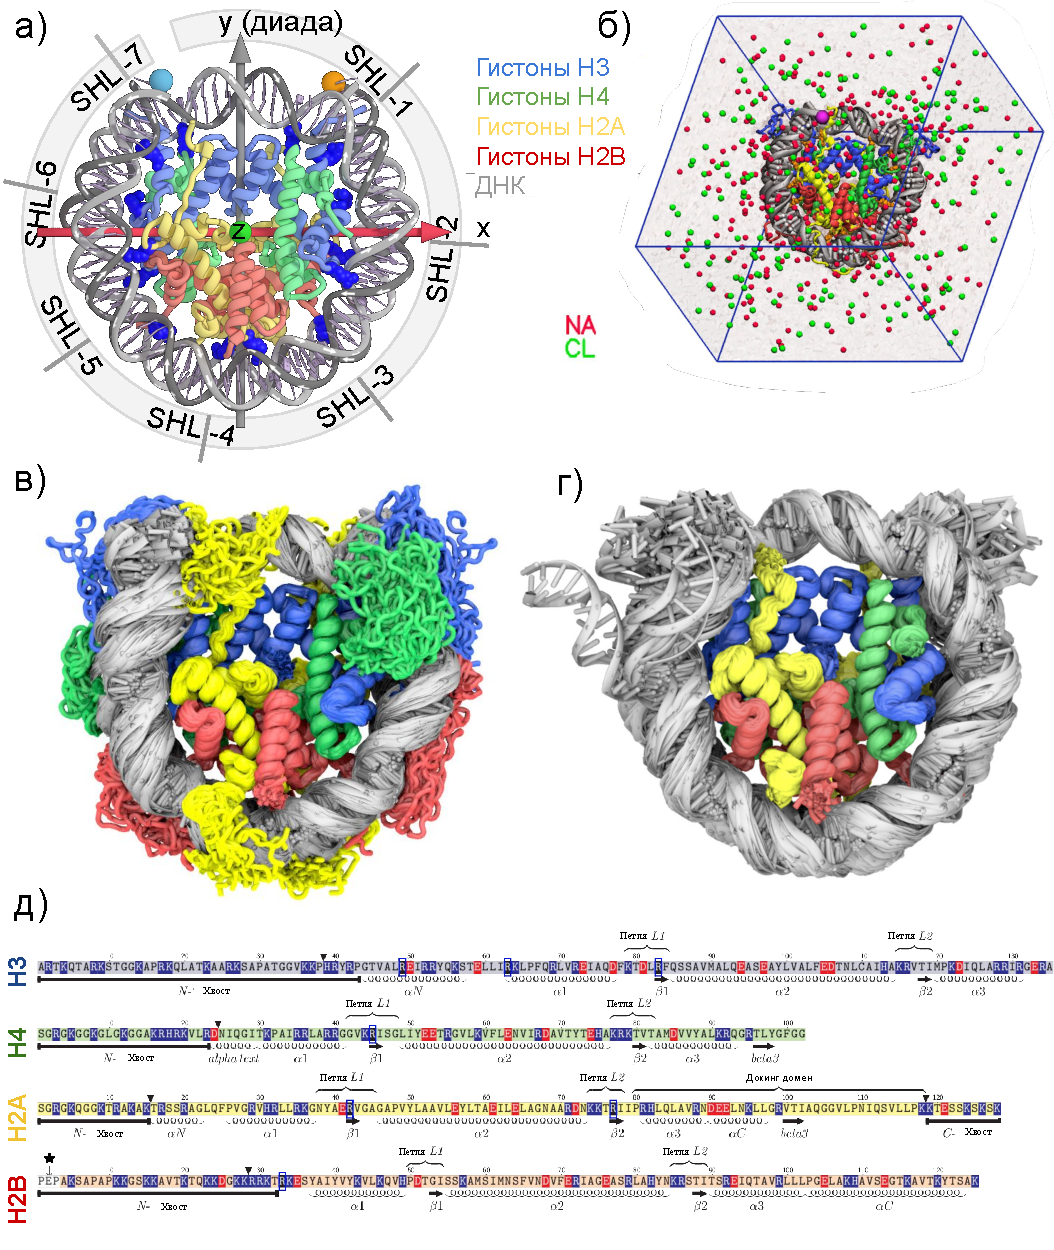
\includegraphics[width=0.95\textwidth]{images/p2/10ms/fig1.pdf}
    \caption[Системы нуклеосом моделируемые на временах более 10 мкс]{Системы нуклеосом моделируемые на временах более 10 мкс. а) Ключевые оси нуклеосомной системы отсчета. б) Вид моделируемой системы в ячейке с растворителем и ионами. c) Наложение кадров системы NCP$_{147} $каждые 100 нс. г) Наложение кадров NCP$^{nt}_{145}$ каждые 100 нс. д) Последовательность коровых гистонов и особенности их вторичной структуры ($ \alpha $ - спирали, $ \beta $ -листы, петли, гибкие хвосты гистонов). $ \blacktriangledown $ отмечает позиции обрезания хвостов в модели с усеченными хвостами; аргинины, боковые цепи которых вставлены малые бороздки ДНК отмечены синими рамками; синим отмечены - положительно заряженные остатки, красным - отрицательно заряженные остатки. $*$ отмечает PEP-конец H2B, который отсутствует в рекомбинантном варианте белка.}
    \label{fig:p2_3:f1}
\end{figure}

\begin{table}[p]
\caption{Список моделируемых систем}
\label{tbl:p2_3:systems}
\begin{threeparttable}
\begin{tabular}{lcp{8cm}c}
\hline
\textbf{Имя}& \textbf{PDB ID}\tnote{a} & \textbf{Описание}&\textbf{Время, мкс}\\ \hline\hline
NCP$_{147}$ & 1KX5 & 147 п.н. псевдосимметричной $\alpha$-сателлитной ДНК, гистоны полной длины в симметричном стартовом состоянии & 13.0  \\ \hline
NCP$^{fixed}_{147}$  & 1KX5 & Такая же как NCP$_{147}$, но C$\alpha$-атомы гистоновых фолдов ограничены в движении &  5.0  \\ \hline
NCP$^{nt}_{147}$ & 1KX5 & Такая же как NCP$_{147}$, но гистоновых хвосты обрезаны\tnote{b} &  10.0  \\ \hline
NCP$^{nt}_{146}$ & 1AOI & 146 п.н. $\alpha$-сателлитная ДНК, обрезанные гистоновые хвосты\tnote{b} & 7.0 \\ \hline
NCP$^{nt}_{145}$ & 3LZ0 & 145 п.н. 601-ой последовательности ДНК, обрезанные гистоновые хвосты\tnote{b} & 13.5  \\ \hline
\end{tabular}
\begin{tablenotes}
     \item[a] Иденификатор структуры, использованной для создания системы, из базы данных PDB.
     \item[b] Сайты обрезки хвостов определены на рис. \ref{fig:p2_3:f1}д.
   \end{tablenotes}
\end{threeparttable}
\end{table}


\subsubsection{Механизмы отворачивания и приворачивания ДНК}

Для анализа отворачивания ДНК от гистонового октамера нами был разработан подход определения количества отвернуты пар нуклеотидов ДНК для каждого кадра траектории. Для каждой пары нуклеотидов вычислялось ее ближайшее расстояние до какой-либо пары нуклеотидов кристаллической структуры. Количество отвернутых пар нуклеотидов с каждого конца определялось как максимальна длина сегмента ДНК от конца ДНК в котором расстояние для всех нуклеотидных пар от любых кристаллических положений было более 7 \AA. На основе данной меры были построены графики зависимости величины отворота ДНК от времени (Рис. \ref{fig:p2_3:f2_new}, Рис. \ref{fig:p2_3:f2}a,б и интерактивные материалы \url{http://intbio.github.io/nucl_MD_15mus/}).

Для систем без гистоновых хвостов ДНК сохраняла исходное привернутое положение в течение начального времени моделирования. Для разных расчетов и сторон нуклеосомы оно колебалось от 0.8 мкс до 4, 6 и более 7 мкс (см. Рис. \ref{fig:p2_3:f2_new}). Для системы с гистоновыми хвостами отворачивание началось на 4-ой микросекунде расчетов. Величина отворота ДНК составляла порядка 12-13 пар нуклеотидов, а в случае систем без хвостов иногда достигала 28 пар нуклеотидов. Рассмотрим в начале механизмы отворота ДНК в системе без хвостов. Анализ стабильных контактов гистонов и нуклеосом показывает, что конец ДНК в нуклеосомном коре формирует плотные контакты и удерживается взаимодействиями с аминокислотными остатками H3 гистона, в особенности H3Y41, H3R42, H3T45, которые находятся в области, которую мы назовем областью ``защелки'' концов ДНК \ref{fig:p2_3:f6}. Плотные взаимодействия в этой области удерживают конец ДНК в NCP. При отвороте ДНК данные взаимодействия нарушаются и ДНК переходит во флуктуирующее состояние, в котором величина отворота быстро меняется в наносекундном диапазоне (см. Рис. \ref{fig:p2_3:f2_new}, состояние \textbf{2}). В некоторых случаях плотные контакты застежки с ДНК восстанавливаются и система переходит в кристаллоподобное состояние (например в системе NCP$_{145}^{nt}$ на третьей наносекунде моделирования). Однако может произойти реконфигурация области защелки в гистоне H3 в состояние, не способное к плотному связыванию ДНК. Это приводит к тому, что флуктуационное состояние становится более долгоживущим и сопровождается также флуктуациями области H3 хвоста (см. Рис. \ref{fig:p2_3:f2_new}, состояние \textbf{2b}). Это флуктуационное состояние может разрешаться в кристаллоподобное состояние ДНК, когда остатки H3 смогут сформировать плотные контакты с флуктуирующим концом ДНК. Более детальный визуальный анализ взаимодействия гистона H3 с концом ДНК показал, что стабильное кристаллоподобное состояние ДНК возникает, когда ряд остатков входят в малую бороздку ДНК. В кристаллической структуре это H3R49, H3Y41, H3H39. Интересно, что в нашем моделировании в ряде систем (NCP$_{145}^{nt}$, NCP$_{145}^{nt}$) кристаллоподобное состояние ДНК также реализовывалось в состоянии, когда вместо H3H39 в малую бороздку заходил H3К40, который в кристалле взаимодействует с малой бороздкой другого супервитка (см. Рис. \ref{fig:p2_3:f2_new}, состояние \textbf{1b}). Дальнейшему откручиванию ДНК препятствовал стабильный сайт связывания с гистонов H2A в районе позиции -59, с которой контактируют остатки H2AK75, H2AT76, H2AR77 из L2 петли. На 14-ой микросекунде в системе NCP$_{145}^{nt}$ наблюдался дальнейший отворот до уровне 26-28 отвернутых пар оснований с диссоциацией контактов данного сайта(см. Рис. \ref{fig:p2_3:f2_new}, состояние \textbf{3}). Данный факт требует дальнейшего исследования. Масштаб флуктуаций ДНК в системе без хвостов представлен на рисунках \ref{fig:p2_3:f1}в,г. Важной особенностью является то, что ДНК откручивается не только в плоскости нуклеосомного диска, но и имеет компонент смещения вдоль суперспиральной оси нуклеосомы. Более подробно взаимоотношение смещения конца ДНК вдоль оси Х и Z представлено на рисунке \ref{fig:p2_3:f1}ж. Существенной корреляции между смещениями не наблюдается, однако очевидно, что при больших параметрах отворота наблюдается в основном состояния с некоторым компонентом смещения вдоль оси суперспирали в направление противоположное от внутреннего супервитка ДНК. Данный факт можно объяснить стерическим и электростатическим отталкиванием витков ДНК.

В отличие от систем без гистоновых хвостов, система с хвостами ведет себя несколько по другому (Рис. \ref{fig:p2_3:f1}б,д,е). Мы также наблюдали откручивание до 12-14 пар оснований с конца ДНК, однако существуют существенные отличия. Во-первых, величина отклонения открученных пар нуклеотидов от их кристаллического пути была меньше из-зи того, что гистоновые хвосты оказывали удерживающее воздействие на конформацию ДНК и ее возможность отклонятся в различных направлениях. Во-вторых, флуктуации ДНК между состояниями с различной степенью откручивания были менее выражены по амплитуде, опять же из-за воздействия гистоновых хвостов, главным образом N-хвоста гистона H3 и С-конца гистона H2A. Наличие гистоновых хвостов приводит к расщеплению динамического состояния отворота-приворота 12 концевых нуклеотидов, наблюдаемого в системе без хвостов, на ряд подсостояний определяемых конформацией гистоновых хвостов. Рисунок \ref{fig:p2_3:f1}и иллюстрирует среднее время приворота ДНК из состояний с заданной величиной отворота. Из рисунка видно, что наличие гистоновых хвостов серьезным образом влияет на увеличение времени приворота ДНК. Для величины отворота в 10 пн время возрастает с 20-40 нс до $\sim$100 нс. Гистоновые хвосты также существенным образом влияют на механизм отворачивания ДНК. Мы наблюдали, что область ``защелки'' H3 гистона также, как и в случае системы без хвостов, теряет контакты с сегментом ДНК вблизи входа-выхода, однако, потери этих контактов способствует внедрение N-конца гистона H3 между супервитками ДНК. Хвост H3 с одной стороны образует дополнительные контакты с ДНК, но с другой стороны способствует замещению стабильных контактов с область H3-``защелки''. Этот же эффект приводит к тому, что в отличие от системы без гистоновых хвостов, хвост H3 может препятствовать быстрому привороту ДНК из отвернутого положения в привернутое.

Более подробно динамика взаимодействия ДНК с H3-``защелкой'' и взаимодействие хвостов гистонов с концами нуклеосомной ДНК представлена на рисунке \ref{fig:p2_3:f3}.

\begin{figure} [H]
    \centering
    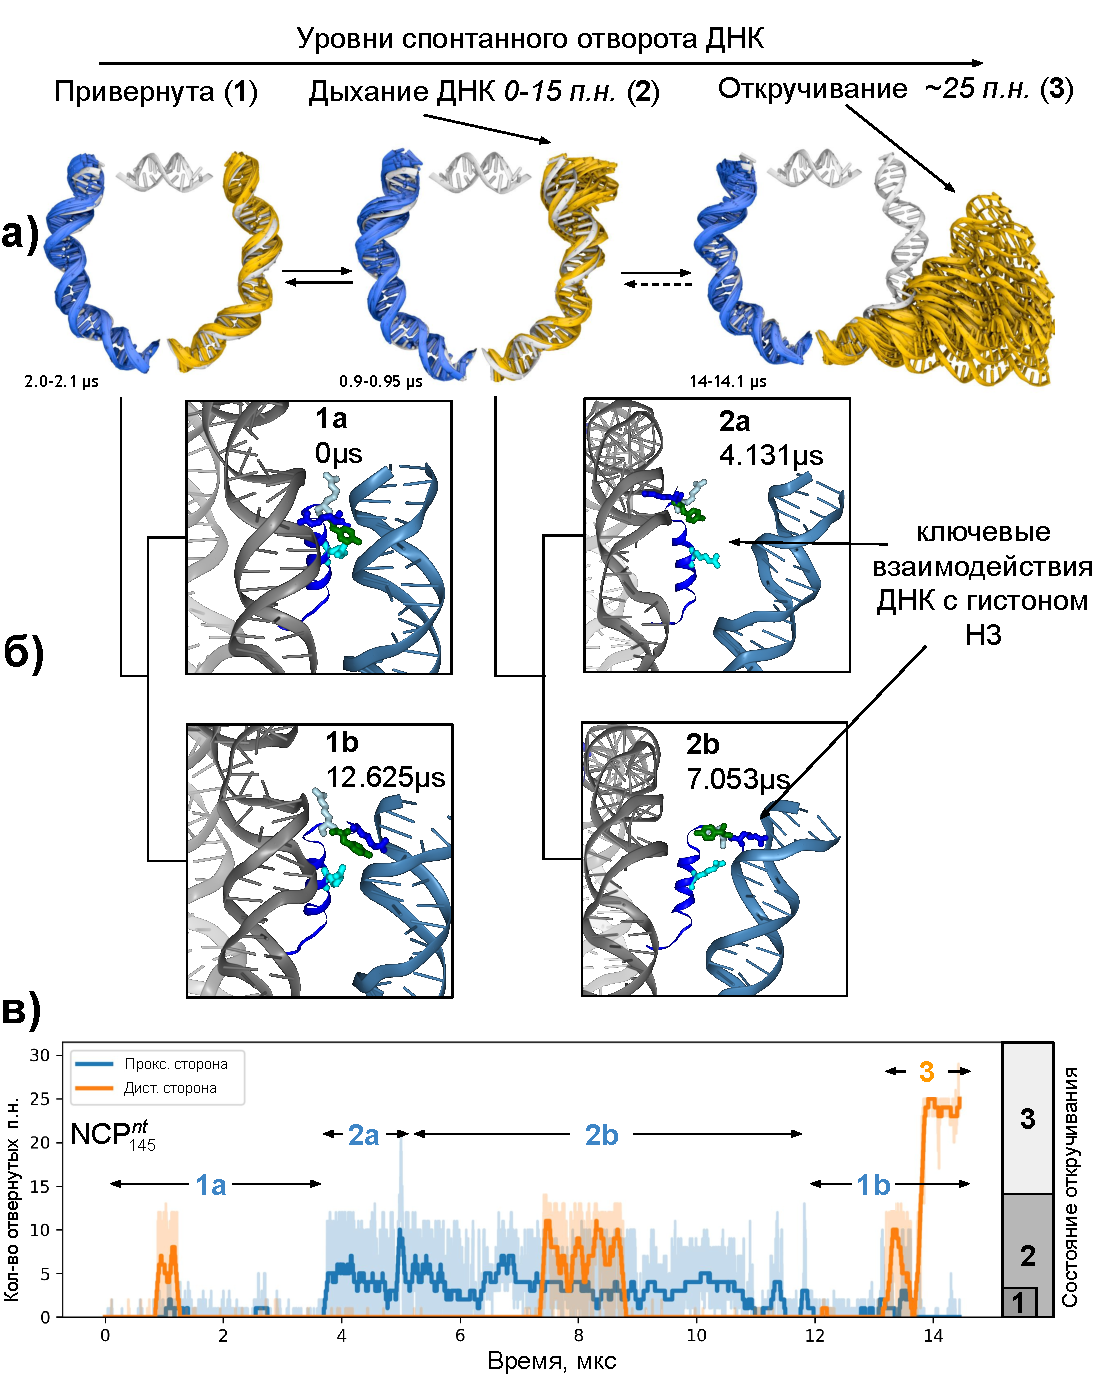
\includegraphics[width=\textwidth]{images/p2/10ms/fig2_new.pdf}
    \caption[Динамика отворота ДНК в нуклеосоме с укороченными гистоновыми хвостами]{Динамика отворота ДНК в нуклеосоме с укороченными гистоновыми хвостами (наблюдаемая в системе NCP$^{nt}_{145}$). Количество пар нуклеотидов отвернутых от октамера гистонов как функция времени моделирования представлена снизу. Критерий отворота ДНК  --  смещение центра пары оснований более, чем на 7 \AA{} от положений оснований в исходной структуре. Наблюдается три состояния \textbf{1-3} (изображены сверху). Для состояний \textbf{1} и \textbf{2} наблюдаются подсостояния, связанные с реориентацией H3 $\alpha$N спирали и области H3-``застежки'' (средний ряд изображений).}
    \label{fig:p2_3:f2_new}
\end{figure}



\begin{figure} [H]
    \centering
    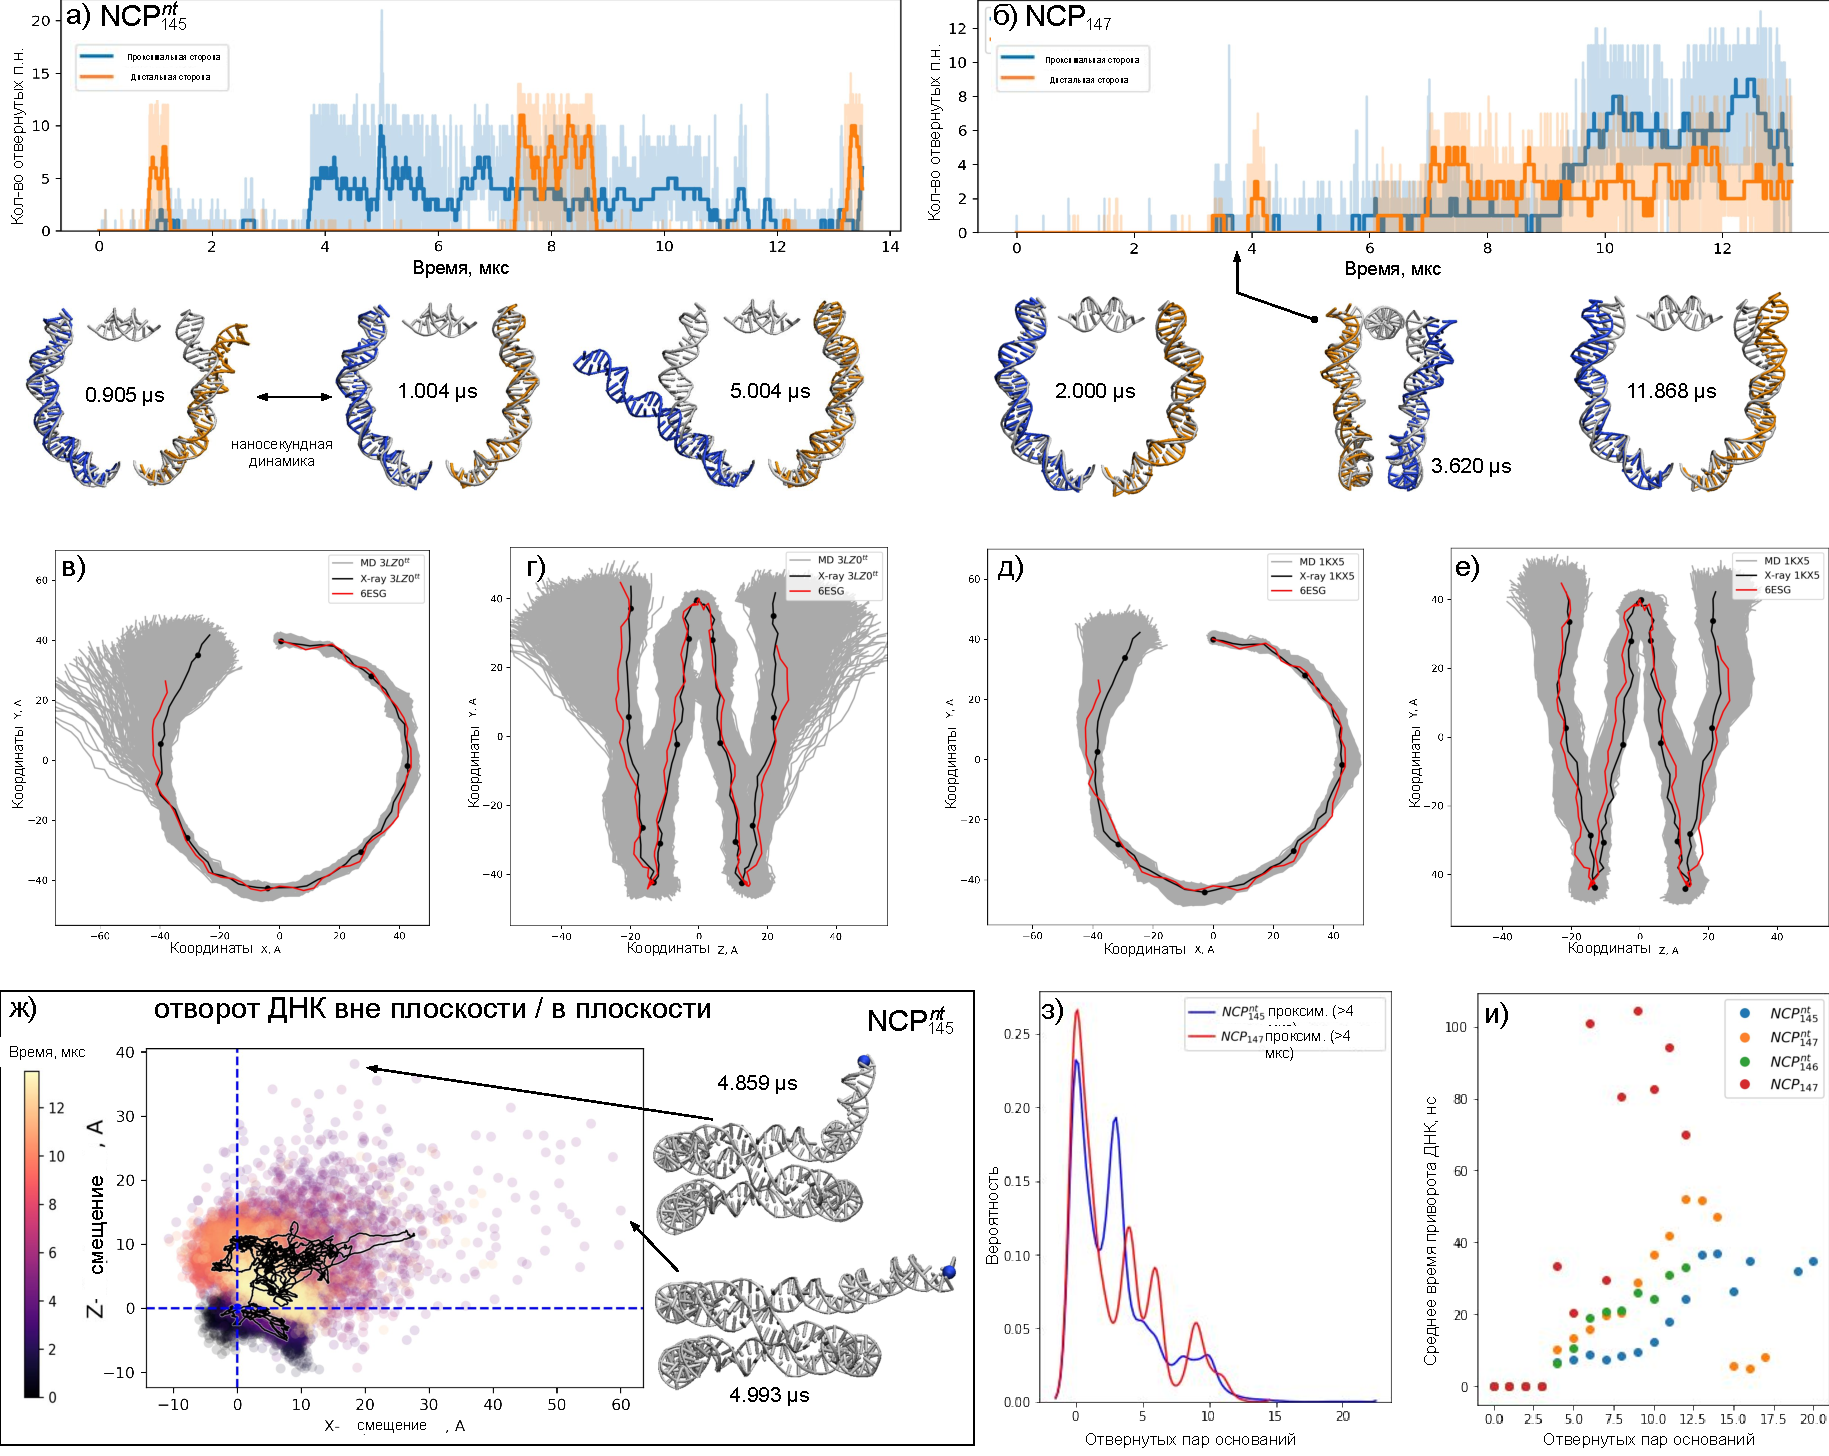
\includegraphics[width=\textwidth]{images/p2/10ms/fig2.pdf}
    \caption[Сравнение характеристик отворота ДНК в нуклеосомах с и без гистоновых хвостов]{Сравнение характеристик отворота ДНК в нуклеосомах с и без гистоновых хвостов. а)-б) отворот ДНК с течением времени для NCP$^{nt}_{145}$ и NCP$_{147}$, определенных как смещение центра пары оснований более, чем на 7 \AA{} от положений оснований в исходной структуре. в-е) Проекции центров пар оснований ДНК на различные плоскости СКН. ж) Смещение проксимального конца ДНК в ходе МД. з) Распределений вероятности отворота ДНК. и) Среднее время приворота ДНК из состояния с определенным отворотом.}
    \label{fig:p2_3:f2}
\end{figure}





\begin{figure}[H]
    \centering
    %DNA ends are coupled to the inner DNA dyre via a  histone H3 residues.
    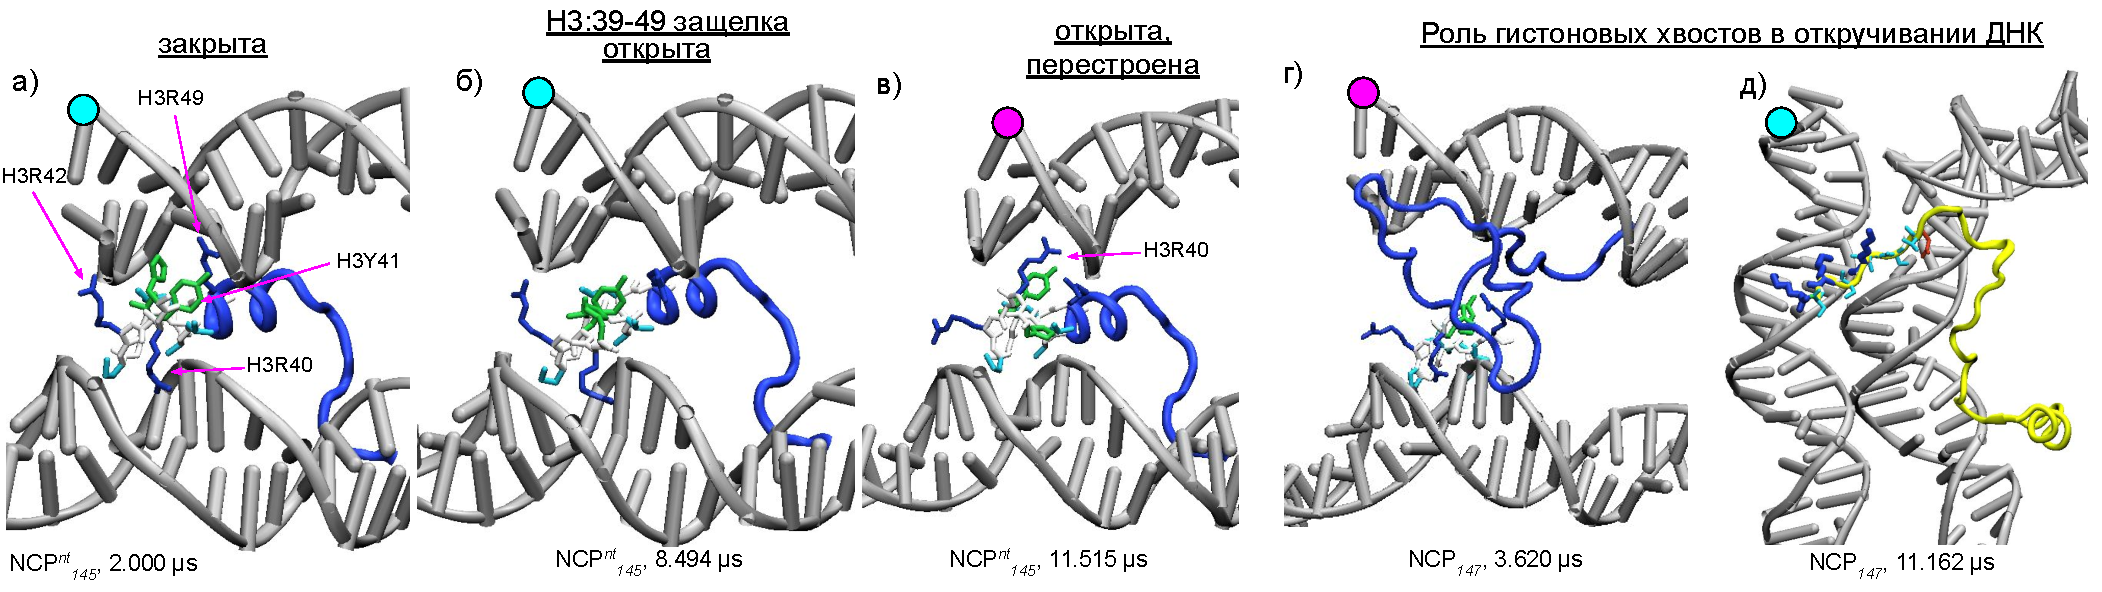
\includegraphics[width=\textwidth]{images/p2/10ms/fig3.pdf}
    \caption[Динамика ``защелки'' концов ДНК фрагментом гистона H3]{Динамика ``защелки'' концов ДНК фрагментом гистона H3}
    \label{fig:p2_3:f3}
\end{figure}



Каковым может быть функциональное значение отворачивания ДНК концов от гистонового кора? С одной стороны предполагается, что отворачивание ДНК необходимо для связывания различных факторов транскрипции \cite{li_rapid_2005}. В нашем моделировании для системы с гистоновыми хвостами ДНК не достигала такой степени отворота. Однако плотное взаимодействие хвостов с ДНК скорее всего распространится и на более существенные степени отворота ДНК. Таким образом, мы предполагаем, что важным фактором для определения доступности ДНК для транскрипционных факторов будет не только отворот ДНК, но и взаимодействия ДНК с гистоновыми хвостами. Другим возможным эффектом отворачивания ДНК является влияние изменение конформации нуклеосомальной ДНК на возможную укладку нуклеосом на супрануклеосомном уровне. Для оценки данных эффектов мы провели моделирование, в котором генерировали фибриллы из 10 нуклеосом, соединяя прямыми отрезками линкерной ДНК длиной 17 п.н. случайно выбранные  кадры из траекторий. Таким образом, можно было получить ансамбль конформаций нуклеосомных фибрилл и оценить распределение длин между концами фибрилл (Рис. \ref{fig:p2_3:f4}). По сравнению с фибриллами построенными на основе кристаллической структуры, фибриллы построенные с учетом флуктуаций концов коровой ДНК демонстрировали в среднем расстояние между концами на 10-15 нм больше. Ширина самого распределения составляла около 20 \AA. Таким образом, можно сделать вывод о том, что динамика концов ДНК, во-первых, ``разрыхляет'' супрануклеосомную структуру хроматина, а, во-вторых, обеспечивает достаточную конформационную гибкость фибриллы в пределах тепловых колебаний ($\sim$kT). 



\begin{figure}[H]
    \centering
    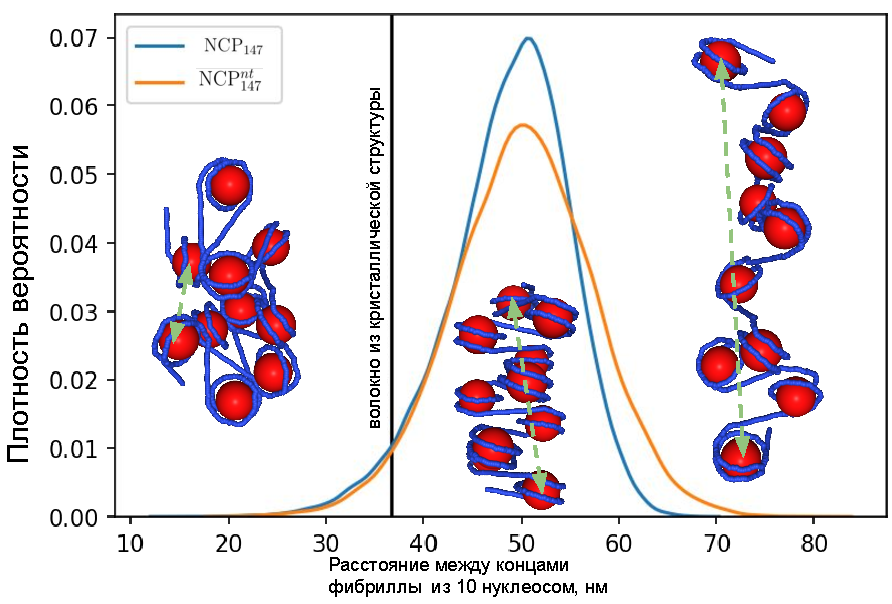
\includegraphics[width=\textwidth]{images/p2/10ms/fig4.pdf}
    \caption[Влияние динамики ДНК на структуру хроматиновых фибрилл]{Влияние динамики ДНК на структуру хроматиновых фибрилл}
    \label{fig:p2_3:f4}
\end{figure}


\subsubsection{Динамика кручения ДНК в нуклеосоме}

Интересным фактом в ходе моделирования явилось наблюдение релаксации дефекта кручения ДНК внутри нуклеосомного кора в системе NCP$_{147}^{nt}$. Дефект кручения ДНК в этой системе, основанной на 601-ой последовательности ДНК, располагается в районе SHL $\pm$5. По сравнению с нуклеосомами на основе альфа-сателлитной ДНК, ДНК в районе этого положения растянута на 1 нуклеотид, при этом совершает то же самое количество оборотов (см. рисунок \ref{fig:p2_3:f5}г). В ходе моделирования мы наблюдали резкий перескок регистра ДНК из кристаллоподобного состояния (Рис. \ref{fig:p2_3:f5}б) в состояние, где нуклеотиды начиная с нуклеотида номер -54 сместились в сторону диады нуклеосомы. Рисунок  \ref{fig:p2_3:f5}д иллюстрирует то, что данный сдвиг регистра ДНК далее произошел для всего конца ДНК, начиная приблизительно с нуклеотида -50. Таким образом около 20 нуклеотидов с проксимального конца ДНК испытали вращательное движение внутри нуклеосомного кора. Любопытным является изучение деталей данного механизма. Рассмотрение динамики отворачивание ДНК свидетельствует о том, что релаксация дефекта кручения произошла в области, которая не была затронута отворотом ДНК (Рис. \ref{fig:p2_3:f2}а). В то же время нельзя исключить, что отворот концов ДНК способствовал релаксации дефекта и его распространению вдоль ДНК. С точки зрения стальных контактов в системе NCP$_{145}^{nt}$ в районе SHL -6 в течение первой микросекунды моделирования наблюдался стабильный контакт нижней цепи ДНК в положении -58 с H2AT76 и верхней цепи ДНК в положении -54 с H2BS56. При анализе 10 микросекунды моделирования на предмет стабильных контактов между нуклеотидами и аминокислотами оказалось, что первый контакт остался неизменным, а второй контакт сместился на нуклеотид за номером -55. Таким образом, релаксация данного дефекта кручения была в некотором роде асимметрична. В большей степени наблюдалось сдвиг регистра контактов для верхней цепи ДНК. Интересным фактом является то, что как недавно было показано в структурных работах по изучению механизмов работ ремоделеров нуклеосом семейства ISWI и SWI/SNF, именно, верхняя цепь ДНК изменяет свое положение на нуклеосомном коре в первую очередь при связывании АТФ субъединицы ремоделера \cite{li_mechanism_2019}.

Еще одним интересным фактом сопровождающим релаксацию дефекта кручения ДНК в районе SHL -5 является деформация в этот момент спирали $\alpha2$ H2A гистона с отгибом ее С-конца в сторону центра нуклеосомного кора. С-конец данной спирали связан с сайтом связывания ДНК в районе SHL -5.5 и, вероятно, участвует в ослаблении контактов ДНК с гистоновым кором, которое помогает релаксации дефекта кручения.


\begin{figure}[H]
    \centering
    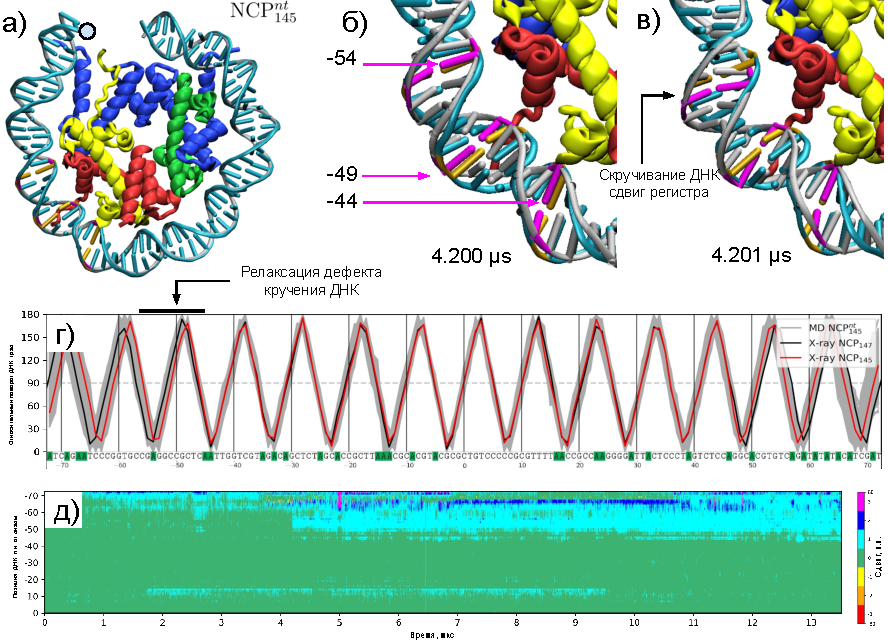
\includegraphics[width=\textwidth]{images/p2/10ms/fig5.pdf}
    \caption[Динамика кручения ДНК в нуклеосоме]{Динамика кручения ДНК в нуклеосоме. а) Структура проксимального супервитка нуклеосомы в начальный момент. Кристаллическая форма ДНК изображена голубым цветом, серым цветом ДНК в ходе МД моделирования. Оранжевым цветом отмечены пары нуклеотидов, которые участвуют изменяют положение на нуклеосоме. б) Кадр траектории до прокручивания ДНК. в) Кадр траектории после прокручивания ДНК. г) График параметра относительного кручения (relative twist) ДНК на нуклеосоме. д) Иллюстрация сдвига в положении нуклеотидов для верхней цепи ДНК относительно положения в кристаллической структуре.}
    \label{fig:p2_3:f5}
\end{figure}



\subsubsection{Динамика контактов ДНК-белок в нуклеосоме}

Наличие траекторий молекулярной динамики позволяет достаточно точно описать взаимодействия гистонов с ДНК на уровне контактов отдельных атомов, аминокислот, нуклеотидов. Причем в отличие от анализа кристаллических структуру имеется возможность оценить устойчивость и динамическую подвижность тех или иных контактов. Нами был проведен анализ стабильных контактов между аминокислотными остатками гистонов и нуклеотидами ДНК. Для изначального анализа была выбрана система NCP$_{147}$ в течение первой микросекунды моделирования, когда отворота ДНК не наблюдалась. Также поскольку система является псевдосимметричной мы учитывали только те контакты, которые присутствовали с обеих сторон нуклеосомы. Результат анализа приведена на рисунке \ref{fig:p2_3:f6}. Данные график иллюстрирует все основные особенности связывания ДНК с гистонами. Обратим внимание на две особенности, которые по нашему мнению имеют функциональное значение. Количество контактов, которые образует верхняя цепь ДНК значительно меньше, контактов которые образует нижняя цепь ДНК. Предполагаем, что это как раз может иметь значение при передвижении нуклеосом вдоль ДНК АТФ-зависимыми ремоделерами, которые как было показано недавно в первую очередь вытягивают и деформируют верхнюю цепь ДНК. Второй интересный момент связан с наличием области H3 гистона, которую мы называем ``защелкой'', которая взаимодействует как с концом коровой ДНК, так и с областью вблизи диады - около положения -9. Отметим, что вблизи положения -9 в геномных исследованиях по позиционированию нуклеосом наблюдается необычный сигнал - там чаще встречаются нуклеотиды A/T, хотя по общему правилу нуклеосомы предпочитают в области изгиба ДНК в сторону большой бороздки нуклеотиды G/C \cite{davey_does_2013}. Данные факт может отчасти объясняться плотным взаимодействием H3R40 внутри малой бороздки ДНК с электроотрицательным группами A/T оснований.


\begin{figure} [H]
    \centering
    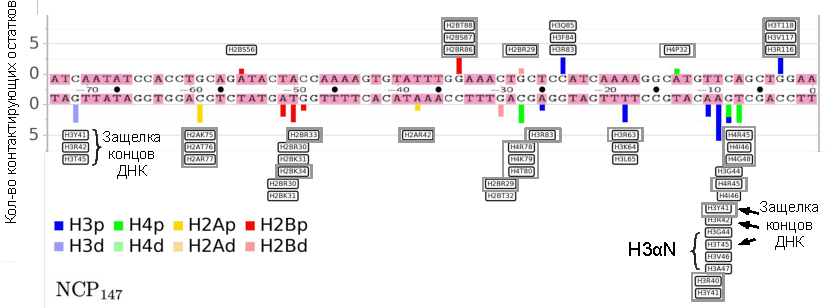
\includegraphics[width=\textwidth]{images/p2/10ms/fig6.pdf}
    \caption[Стабильные контакты ДНК-гистоны в нуклеосоме]{Стабильные контакты ДНК-гистоны в нуклеосоме. Отмечены контакты между нуклеотидами и аминокислотными остатками, присутствующие в 90\% кадров в системе NCP$_{147}$ в течение первой микросекунды моделирования с обоих симметричных сторон нуклеосомы. В рамках отмечены контакты, которые сохраняются с обоих сторон нуклеосомы в течение всей МД траектории.}
    \label{fig:p2_3:f6}
\end{figure}

\subsubsection{Пластичность гистонового октамера}

Как было описано во введении весьма актуальной темой научных исследований на данный момент является изучение пластичности октамера гистонов. Для исследования данного вопроса нами были построены проекции координат атомов $\alpha 2$-спиралей гистонов на плоскость нуклеосомного диска (Рис. \ref{fig:p2_3:f7}. Видно, что спирали испытывают флуктуации в пределах от нескольких до 5-6\AA. Особенно выделяются флуктуации концов C-концов спиралей гистона H2A. Недавно методами крио-ЭМ был разрешен ряд деформированных структур нуклеосомного кора, в частности структура нуклеосомы сжатая вдоль диадной оси на несколько процентов. RMSD кадров  МД траектории относительно данной структуры (Рис. \ref{fig:p2_3:f7}в) показывает, что данная структура зачастую отличается от кадров траектории не более, чем начальная структура самой траектории. Таким образом, можно сделать вывод, что наблюдаемые в эксперименте деформированные состояния нуклеосом находятся, по крайней мере, в рамках отличий, которые мы видим между кадрами траектории на масштабе мультимикросекундного моделирования.

В ряде работ было показано, что дисульфидные сшивки внутри димеров гистонов приводят к изменению функционирования нуклеосом. В частности H3L82C-H4V81C уменьшает термическую диффузию нуклеосом по ДНК и влияет на работу ремоделера SNF2h \cite{bilokapic_histone_2018,bilokapic_structural_2018,sinha_distortion_2017}. Расстояние между С-$\alpha$ атомами данные остатков изображена на рисунке \ref{fig:p2_3:f7}г. Оно колеблется в пределах от 6,1-8,5\AA. Длина дисульфидной связи составляет около 2,05\AA, расстояние между С-$\alpha$-атомом и атомом серы в стандартной конформации цистеина составляет 2,81\AA и не меняется при вращении торсионных углов. Таким образом максимальное расстояния между С-$\alpha$-атомами у остатков цистеина, связанных дисульфидной связью, составляет 7,67\AA. Следуя данным расчетам, видим, что дисульфидная сшивка будет препятствовать некоторым конформациям, наблюдаемым в динамике.

Для того, чтобы дополнительно изучить влияние пластичности октамера на динамику ДНК, мы провели расчеты, в которых $\alpha 2$-спирали гистонов были зафиксированы. Анализ флуктуационной динамики ДНК показал (см. рисунок \ref{fig:p2_3:f7}е), что у системы с фиксированными $\alpha$-спиралями подвижность ДНК была снижена на всем ее протяжении. Данные эффект требует дальнейшего изучения, однако можно предположить, что уменьшение подвижности ДНК отрицательно сказывается на возможности ремоделирования и скольжения нуклеосом.



\begin{figure} [H]
    \centering
    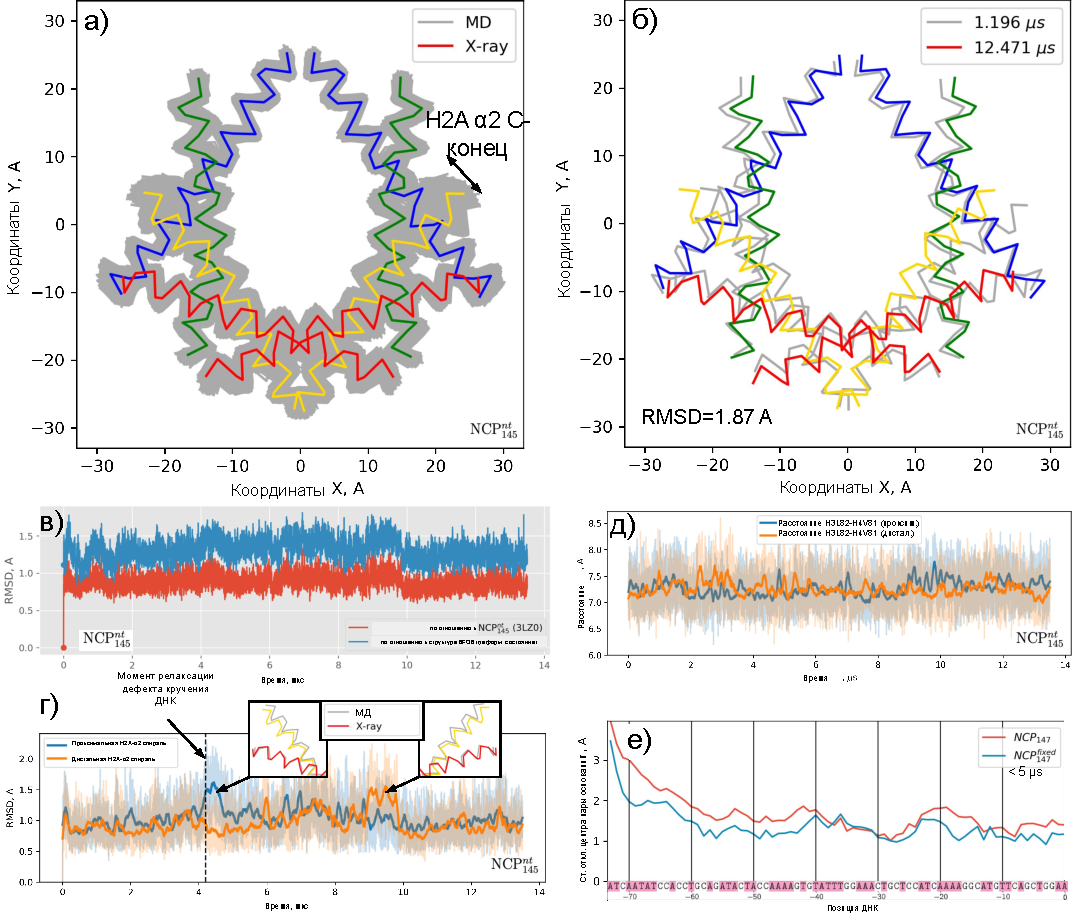
\includegraphics[width=\textwidth]{images/p2/10ms/fig7.pdf}
    \caption[Пластичность гистонового октамера]{Пластичность гистонового октамера. а) Наложение проекций координат С$\alpha$-атомов $\alpha 2$-спиралей гистонов в плоскости нуклеосомального диска из кадров МД траектории. б) Аналогичные проекции координат С$\alpha$-атомов для двух кадров с максимально различным RMSD. в) RMSD $\alpha 2$-спиралей гистонов в ходе МД относительно исходной структуры и структуры 6FQ6, полученной крио-ЭМ, с деформированной конформацией ядра нуклеосомы. г) Эволюция RMSD спирали $\alpha 2$ гистона H2A. д) Расстояние между остатками, которые подвергаются дисульфидным сшивкам в ряде экспериментов. e) Сравнение флуктуаций пар оснований ДНК в системах с закрепленными и незакрепленными $\alpha 2$-спиралями гистонов.}
    \label{fig:p2_3:f7}
\end{figure}

\subsubsection{Аллостерическая связь откручивания ДНК и конформации ДНК около диады}

Область ``застежки'' гистона H3 взаимодействует одновременно с двумя супервитками ДНК. Это наблюдение известно достаточно давно. Например, Horn et al. в своих экспериментах наблюдали, что SIN мутация гистона H4R25C взаимодействующая в положении SHL $\pm$0.5 приводит к ухудшению возможности компактизации нуклеосомальных фибрилл. Они предположили, что одним из возможных механизмов является дестабилизации концов нуклеосомальной ДНК в виду коммуникации области SHL $\pm$0.5 с областями SHL $\pm$6.5 посредством H3 $\alpha$N-спирали. Однако, Flaus et al. предположили, что этот эффект может объясняться увеличением мобильности нуклеосом и их смещению относительно исходных позиций \cite{flaus_sin_2004}. Тем не менее, нам было интересно рассмотреть в нашем моделировании возможные эффекты коммуникации областей SHL $\pm$0.5 и SHL $\pm$6.5. На рисунке \ref{fig:p2_3:f9} приведен сравнительных анализ откручивания ДНК и деформации ДНК в различных положениях от времени для системы NCP$_{147}$. Любопытным является факт, что вслед за откручиванием ДНК, зачастую область ``защелки'' гистона H3 теряет свои контакты не только с концом ДНК, но и с областью нижнего супервитка.
Такой случай изображен на панели \ref{fig:p2_3:f9}в. Потеря контактов с нижним супервитком ДНК в свою очередь ведет к деформации ДНК в этой области и к ее усиленным флуктуациям. Можно предположить, что наличие флуктуация в нижнем супервитке будет способствовать прохождению через нуклеосому дефектов скручивания ДНК.

В результате анализа приведенного в данном разделе нами выдвигается предположение о наличие динамической (аллостерической) связи между откручиванием ДНК и скольжению нуклеосом вдоль ДНК по механизму продвижения дефектов кручения. Откручивание концов коровой ДНК, во-первых, помогает образованию и прохождению дефектов скручивания вблизи концов ДНК, а, во-вторых, способствует дестабилизации ДНК в районе диады, что также, вероятно, помогает прохождению дефектов скручивания далее через нуклеосомную ДНК.



\begin{figure} [H]
    \centering
    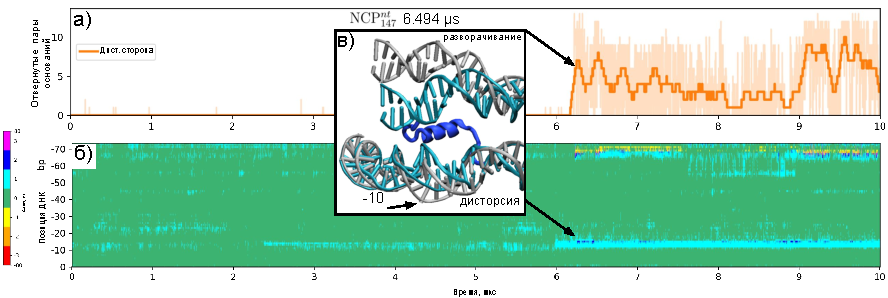
\includegraphics[width=\textwidth]{images/p2/10ms/fig9.pdf}
    \caption[Аллостерическая связь откручивания ДНК и конформации ДНК около диады]{Аллостерическая связь откручивания ДНК и конформации ДНК около диады. а) График откручивание ДНК от времени в ходе МД моделирования. б) График смещения нуклеотидов относительно кристаллической структуры.}
    \label{fig:p2_3:f9}
\end{figure}





\subsection{Благодарности}

Работа данного раздела поддержана грантами Российского научного фонда № 18-74-10006 (атомистическое моделирование нуклеосом и разработка и анализ траекторий нуклеосом), грантами Российского фонда фундаментальных исследований № 20-34-70039 (моделирование структуры супрануклеосомальных фибрилл) и № 19-34-51053 (метода анализа взаимодействий белков и нуклеиновых кислот). Исследования проводились на оборудовании коллективных исследовательских установок вычислительных ресурсов высокопроизводительных вычислений МГУ им. М.В. Ломоносова.


\section{Выводы главы \ref{part2_supermd}}
В данной главе на примере моделирования нуклеосом продемонстрированы возможности современных технологий суперкомпьютерного моделирования динамики биомакромолекулярных систем в атомистическом приближении на микросекундных временных масштабах. Проанализирована конформационная подвижность как коровых частиц нуклеосом (октамер гистонов + 147 пар нуклеотидов ДНК), так и нуклеосом с линкерной ДНК (октамер гистонов + 187 пар нуклеотидов ДНК). Изучена динамика хвостов и внутренняя подвижность глобулярных доменов гистонов, связь динамики белка и ДНК. Впервые в равновесной молекулярной динамике наблюдалась частичная диссоциация и реассоциация (отворот) ДНК от белкового октамера, изменение ориентационного положения ДНК, выпячивание ДНК вблизи входа-выхода в нуклеосому. На основании моделирования могут быть сформулированы следующие научные выводы и гипотезы:

\begin{itemize}
    \item Электростатическое отталкивание двух сегментов линкерной ДНК является одним из факторов, которые влияют на конформацию ДНК и углы входа-выхода ДНК из ядра нуклеосомы.
    \item В процессе спонтанного ступенчатого откручивания/прикручивания ДНК в нуклеосоме последовательно теряются стабильные взаимодействия ДНК с гистонами. Конформация ДНК подвержена значительным флуктуациям в наносекундном диапазоне. В переходе нуклеосом из кристаллоподобного состояния в состояние с отвернутой ДНК ключевую роль играют взаимодействия остатков гистона H3 между двумя супервитками ДНК.
   % \item Показано, что спонтанное откручивание ДНК от нуклеосомы приводит к разрыхлению структуры хроматиновых фибрилл.
    \item Формирование дефектов кручения ДНК в нуклеосоме и конформационные перестройки внутри глобулярных частей гистонового октамера, происходящие на микросекундных временах, указывают на возможность скольжения нуклеосом вдоль ДНК по винтовому механизму и транслокацию ДНК вдоль октамера.
    \item Диссоциации концов нуклеосомальной ДНК от гистонового октамера наблюдается на временах порядка 10 мкс. 
  %  \item Гистоновые хвосты в нуклеосоме активно взаимодействуют с коровой и линкерной ДНК, влияют на кооперативность взаимодействия белков хроматина с гистоновыми хвостами.
  %  \item Конформационные перестройки внутри глобулярных частей гистонового октамера, происходящие на микросекундных временах, влияют на подвижность ДНК и, вероятно, эффективность транслокации ДНК вдоль октамера.
   % \item Показано наличие аллостерических эффектов между откручиванием концов ДНК в нуклеосоме и стабильности центральной части ДНК, важные с точки зрения передвижения нуклеосом вдоль ДНК.  

\end{itemize}




%\begin{itemize}
 %   \item  Конформация линкерной ДНК в нуклеосомах подвержена значительным флуктуациям, которые влияют на углы входа-выхода ДНК из ядра нуклеосомы, электростатическое отталкивание двух сегментов линкерной ДНК является одним из факторов, влияющих на их конформацию и углы входа-выхода.
 %   \item Процесс спонтанного откручивания/прикручивания ДНК в нуклеосоме является ступенчатым процессом и характеризуется переходом между набором динамических состояний, в которых ДНК последовательно теряет стабильные взаимодействия с гистонами, но при этом ее конформация подвержена значительным флуктуациям в наносекундном диапазоне. Предложена структурно-кинетическая модель перехода нуклеосом из кристаллоподобного состояния в состояние с отвернутой ДНК, ключевую роль в которой играют взаимодействия остатков гистона H3, находящиеся между двумя супервитками ДНК.
 %   \item Показано, что спонтанное откручивание ДНК от нуклеосомы приводит к разрыхлению структуры хроматиновых фибрилл.
 %   \item Формирование дефектов кручения ДНК в нуклеосоме может происходить на микросекундных временных диапазонах, что указывает на возможность скольжения нуклеосом вдоль ДНК по винтовому механизму.
   % \item Гистоновые хвосты в нуклеосоме активно взаимодействуют с коровой и линкерной ДНК, влияют на кооперативность взаимодействия белков хроматина с гистоновыми хвостами.
   % \item Конформационные перестройки внутри глобулярных частей гистонового октамера, происходящие на микросекундных временах, влияют на подвижность ДНК и, вероятно, эффективность транслокации ДНК вдоль октамера.
   % \item Показано наличие аллостерических эффектов между откручиванием концов ДНК в нуклеосоме и стабильности центральной части ДНК, важные с точки зрения передвижения нуклеосом вдоль ДНК.  
%\end{itemize}
 


% \subsection{Положения выносимые на защиту}
% %положения выносимые на защиту
% \begin{enumerate}
%   \item На примере нуклеосом разработаны подходы атомистического суперкомпьютерного моделирования биомакромолекулярных комплексов белков и нуклеиновых кислот, способные описывать и анализировать функциональную динамику молекул в микросекундных временных диапазонах.
%   \item С использованием данных подходов охарактеризована на атомистическом уровне функциональная динамика нуклеосом, важная с точки зрения эпигенетической регуляции функционирования генома, охарактеризованы новые моды динамической подвижности, связанные с частичной диссоциацией ДНК от гистонового октамера, перестройкой взаимодействий гистоновых хвостов, деформацией глобулярных доменов гистонов.
% \end{enumerate}